\documentclass[compress,red]{beamer}
\mode<presentation>
\setbeamertemplate{navigation symbols}{}

\usepackage{pgfpages}
% \setbeameroption{show notes}
% \setbeameroption{show notes on second screen=right}

\usetheme{Warsaw}


%\hypersetup{pdfpagemode=FullScreen} % makes your presentation go automatically to full screen

% define your own colors:
\definecolor{Red}{rgb}{1,0,0}
\definecolor{Blue}{rgb}{0,0,1}
\definecolor{Green}{rgb}{0,1,0}
\definecolor{magenta}{rgb}{1,0,.6}
\definecolor{lightblue}{rgb}{0,.5,1}
\definecolor{lightpurple}{rgb}{.6,.4,1}
\definecolor{gold}{rgb}{.6,.5,0}
\definecolor{orange}{rgb}{1,0.4,0}
\definecolor{hotpink}{rgb}{1,0,0.5}
\definecolor{newcolor2}{rgb}{.5,.3,.5}
\definecolor{newcolor}{rgb}{0,.3,1}
\definecolor{newcolor3}{rgb}{1,0,.35}
\definecolor{darkgreen1}{rgb}{0, .35, 0}
\definecolor{darkgreen}{rgb}{0, .6, 0}
\definecolor{darkred}{rgb}{.75,0,0}

\xdefinecolor{olive}{cmyk}{0.64,0,0.95,0.4}
\xdefinecolor{purpleish}{cmyk}{0.75,0.75,0,0}


\useoutertheme[subsection=false]{smoothbars}


% include packages
\usepackage{subfigure}
\usepackage{multicol}
\usepackage{amsmath}
\usepackage{epsfig}
\usepackage{graphicx}
\usepackage[all,knot]{xy}

\xyoption{arc}
\usepackage{url}
\usepackage{multimedia}
\usepackage{hyperref}
\usepackage{helvet}
\usepackage[polish,english]{babel}
\usepackage[utf8]{inputenc}
\usepackage{multirow}

\newcommand{\backupbegin}{
   \newcounter{framenumberappendix}
   \setcounter{framenumberappendix}{\value{framenumber}}
}
\newcommand{\backupend}{
   \addtocounter{framenumberappendix}{-\value{framenumber}}
   \addtocounter{framenumber}{\value{framenumberappendix}} 
}

%%%%%%%%%%%%5
%\usepackage{geometry}
%\geometry{verbose,letterpaper}
%\usepackage{movie15}
%\usepackage{hyperref}
%%%%%%%

% greetings, introduce yourself


%  \includegraphics[height=5cm]{fig/WRlogo.ps}


\title[White Rabbit \hspace{2em}\insertframenumber/\inserttotalframenumber]
{White Rabbit}

\institute{
   \begin{center}
    Hardware and Timing Section / ~~~ Institute of Electronic Systems \\
    ~~~~~~~~~~~~~~~~~~~~~CERN ~~~~~~~~~~~~~~~~ / Warsaw University of Technology \\
   \end{center}
}
\author{
Maciej Lipi\'{n}ski \\
% on behalf of Maciej Lipi\'{n}ski 
}
\date{15th June 2012 \\ ALBA}



\pgfdeclareimage[height=0.6cm]{wr-logo}{../../figures/logo/WRlogo.ps}
\logo{\pgfuseimage{wr-logo}}
\AtBeginSection[]

\begin{document}

\frame{\titlepage}
%%%%%%%%%%%%%%%%%%%%%%%%%%%%%%%%%%%%%%%%%%%%%%%%%%%%%%%%%%%%%%%%%%%%%%%%%%%%%%%%%%%%%%%%%%%%%%%%%%%%
\begin{frame}<beamer>{Outline}
    \tableofcontents %[currentsection]
\end{frame}

%%%%%%%%%%%%%%%%%%%%%%%%%%%%%%%%%%%%%%%%%%%%%%%%%%%%%%%%%%%%%%%%%%%%%%%%%%%%%%%%%%%%%%%%%%%%%%%%%%%%
\section{Introduction}
\subsection{}
%%%%%%%%%%%%%%%%%%%%%%%%%%%%%%%%%%%%%%%%%%%%%%%%%%%%%%%%%%%%%%%%%%%%%%%%%%%%%%%%%%%%%%%%%%%%%%%%%%%%
\begin{frame}{What is White Rabbit?}

\begin{columns}[c]
	\column{0.8\textwidth}
	  \begin{itemize}
		\item Accelerator's control and timing
		\item International collaboration
		\item Based on well-known technologies
		\item Open Hardware and Open Software
		\item Main features:
		\begin{itemize}
		  \item transparent,  {\bf high-accuracy} synchronization
		  \item low-latency,  {\bf deterministic} data delivery
		  \item designed for  {\bf high reliability}
		  \item plug \& play
		\end{itemize}
	  \end{itemize}
	\column{0.3\textwidth}
		\begin{center}
		\pause
		\hspace{-0.5cm}
		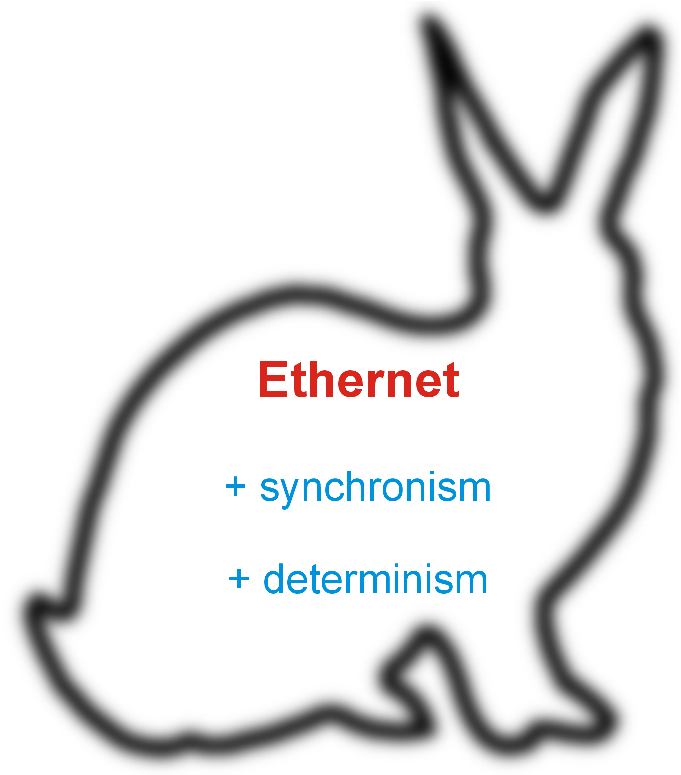
\includegraphics[width=1.1\textwidth]{../../figures/misc/rabbit.eps}
		\end{center}
	\end{columns}

\end{frame}
%%%%%%%%%%%%%%%%%%%%%%%%%%%%%%%%%%%%%%%%%%%%%%%%%%%%%%%%%%%%%%%%%%%%%%%%%%%%%%%%%%%%%%%%%%%%%%%%%%%%
%\section{White Rabbit~~~~}
\subsection{}
%%%%%%%%%%%%%%%%%%%%%%%%%%%%%%%%%%%%%%%%%%%%%%%%%%%%%%%%%%%%%%%%%%%%%%%%%%%%%%%%%%%%%%%%%%%%%%%%%%%%
\begin{frame}{White Rabbit -- enhanced Ethernet}

\begin{columns}[c]
  \column{.47\textwidth}
 

  \begin{itemize}
    \item Few thousands nodes
    \item Copper or fiber medium
    \item Up to 10 km fiber links
    \item Bandwidth: 1 Gbps
    \item WR Switch: 18 ports
    \item Non-WR Devices
    \item Ethernet features (VLAN) \& protocols (SNMP)
  \end{itemize}

  \column{.6\textwidth}
    \begin{center}
    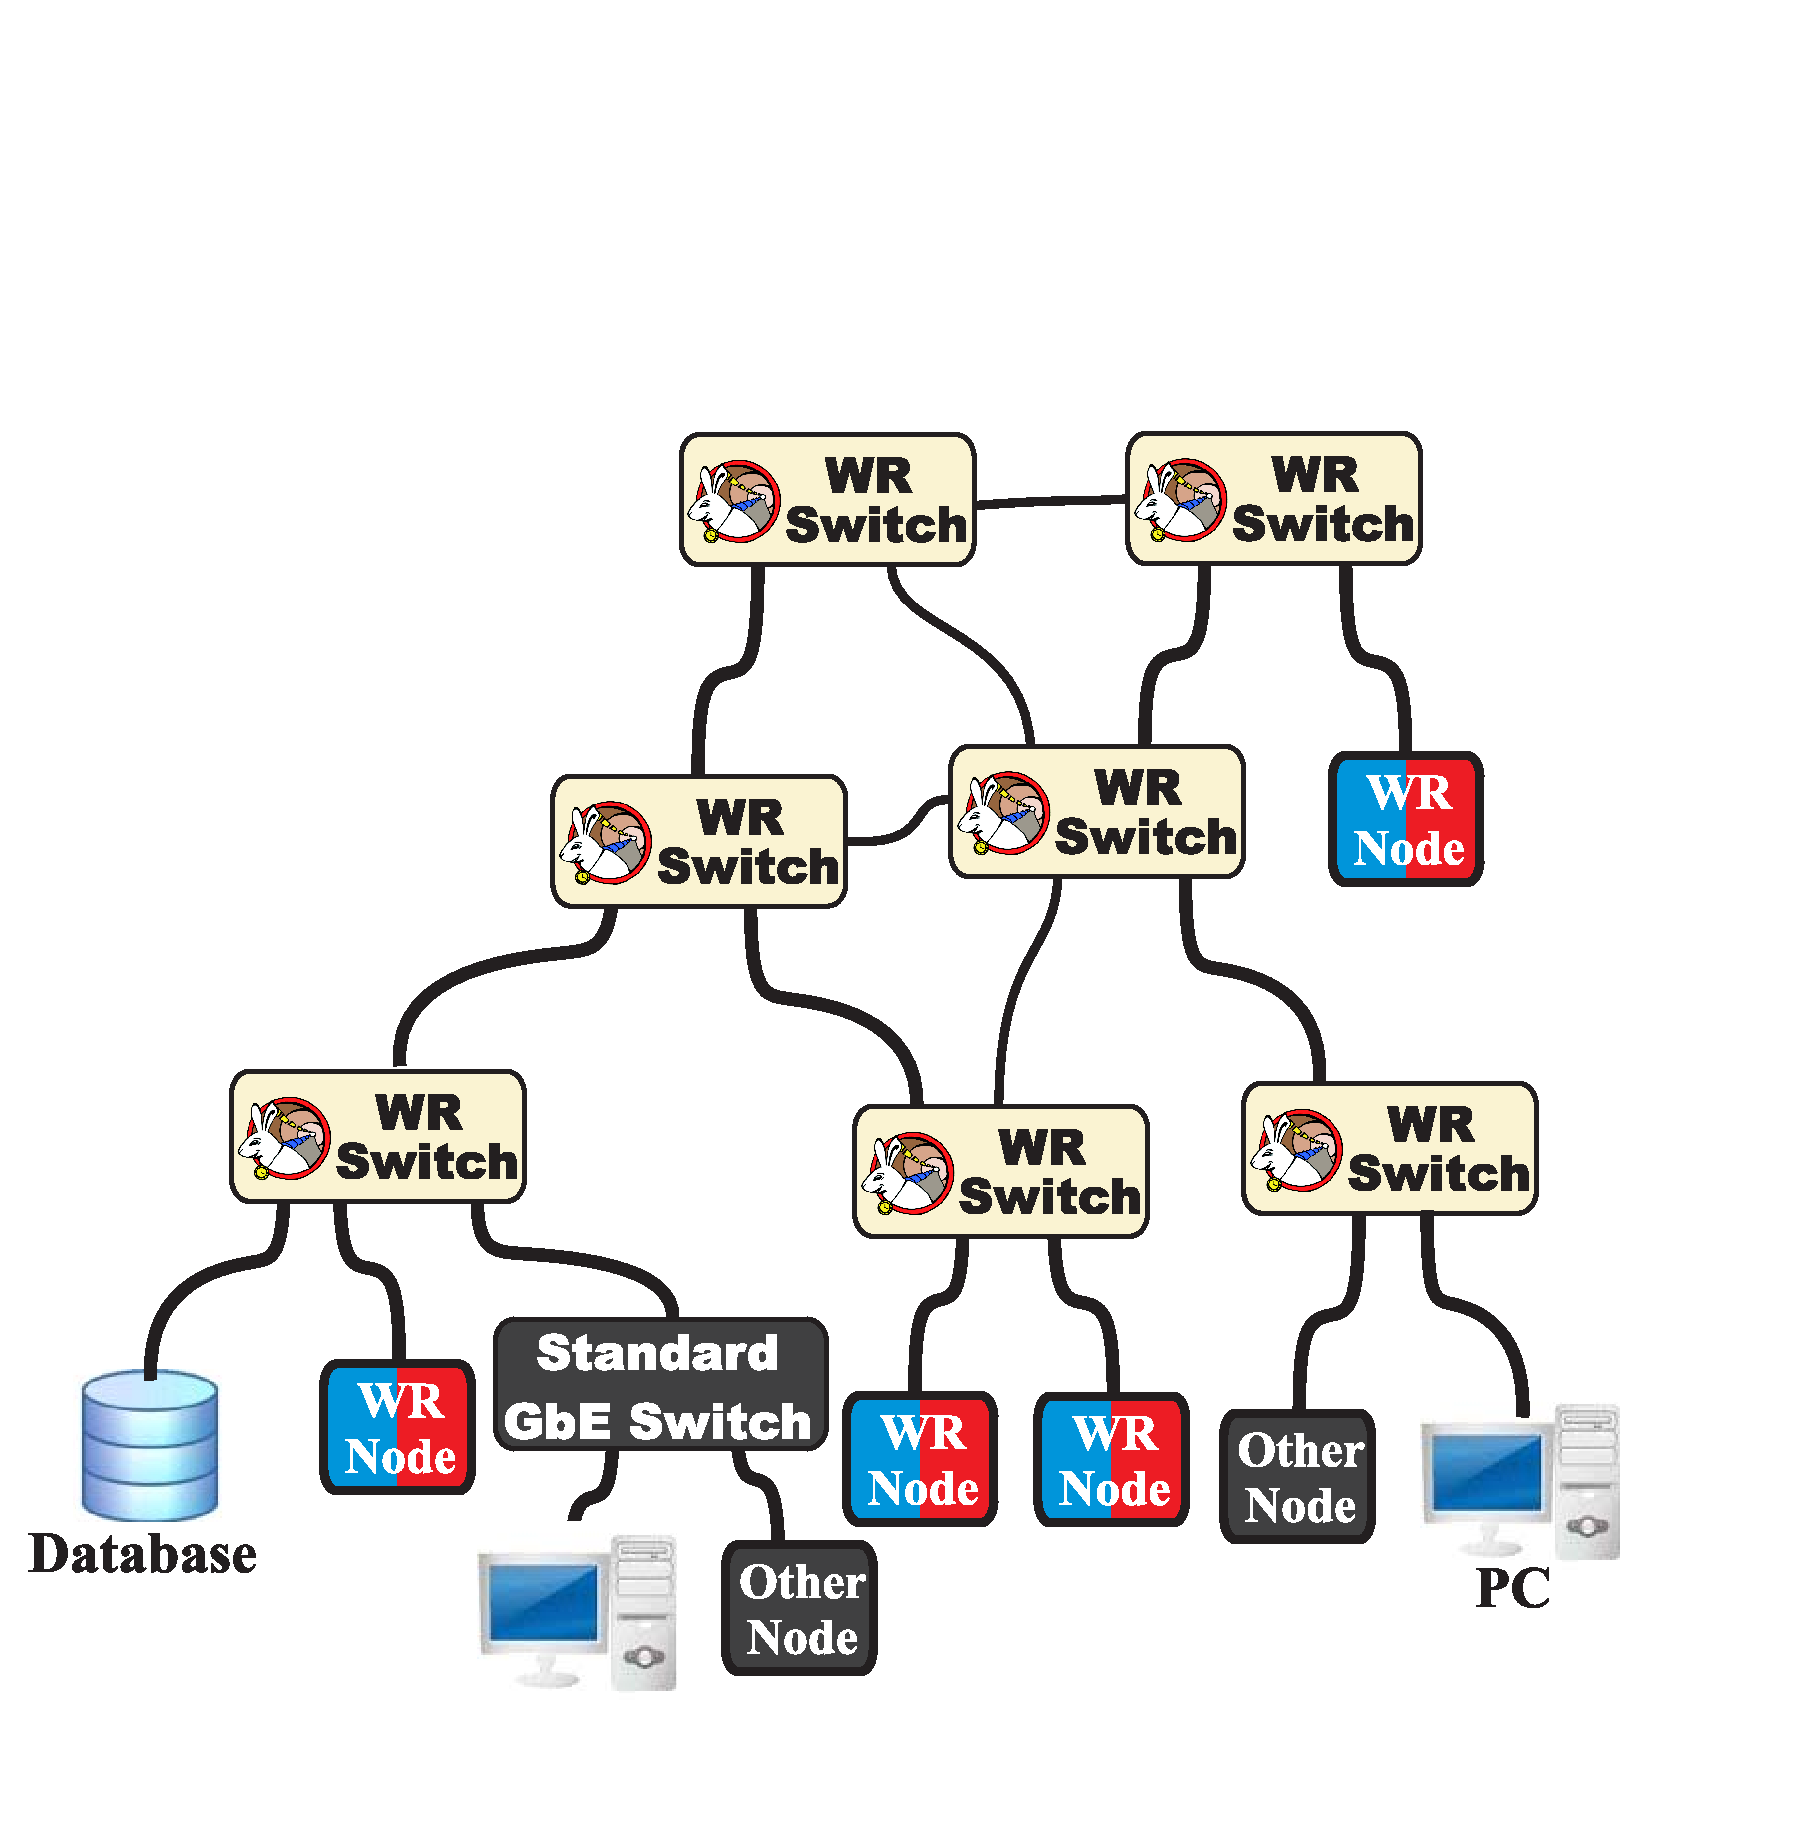
\includegraphics[width=1.0\textwidth]{../../figures/network/WR_network-ethernet.eps}
    \end{center}
\end{columns}

\end{frame}
%%%%%%%%%%%%%%%%%%%%%%%%%%%%%%%%%%%%%%%%%%%%%%%%%%%%%%%%%%%%%%%%%%%%%%%%%%%%%%%%%%%%%%%%%%%%%%%%%%%%
%\section{White Rabbit~~~~}
\subsection{}
%%%%%%%%%%%%%%%%%%%%%%%%%%%%%%%%%%%%%%%%%%%%%%%%%%%%%%%%%%%%%%%%%%%%%%%%%%%%%%%%%%%%%%%%%%%%%%%%%%%%
\begin{frame}{White Rabbit -- enhanced Ethernet}


\begin{columns}[c]
  \column{.47\textwidth}
 
  Two separate services (enhancements to Ethernet) provided by WR: 
  \begin{itemize}
    \item \color{blue!90}{High accuracy/precision synchronization}
    \item \color{red}{Deterministic, reliable and low-latency Control Data delivery}
  \end{itemize}

  \column{.6\textwidth}
    \begin{center}
    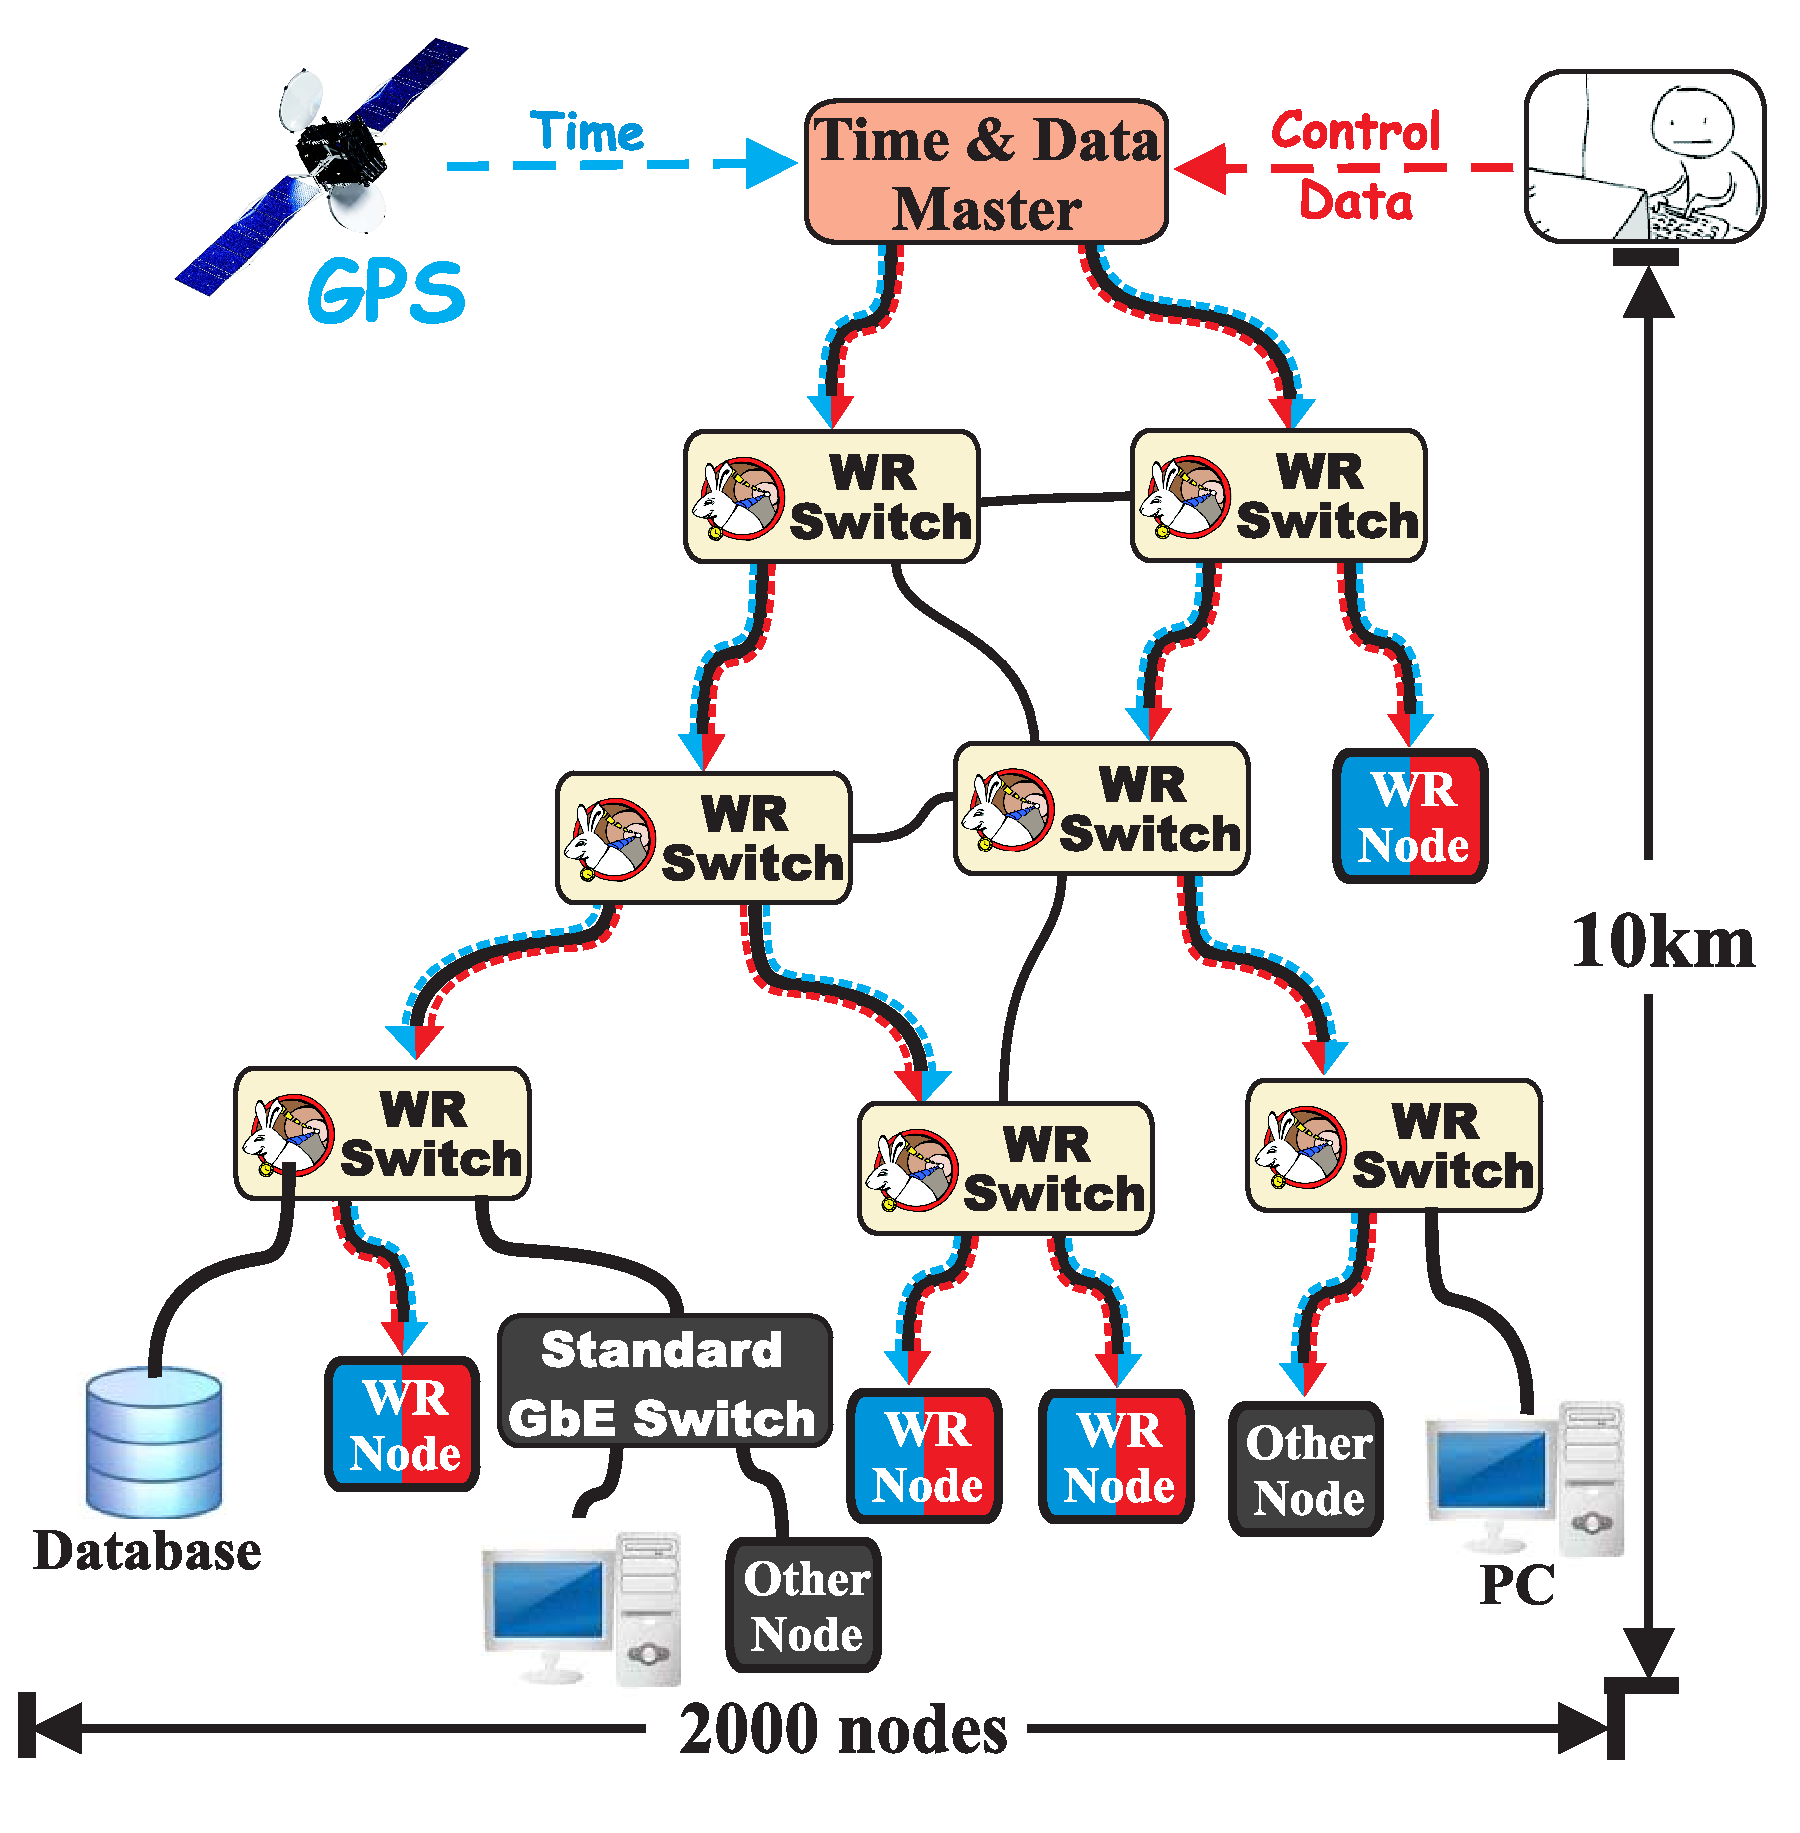
\includegraphics[width=1.0\textwidth]{../../figures/network/wr_network-enhanced.eps}
    \end{center}
\end{columns}

\end{frame}
%%%%%%%%%%%%%%%%%%%%%%%%%%%%%%%%%%%%%%%%%%%%%%%%%%%%%%%%%%%%%%%%%%%%%%%%%%%%%%%%%%%%%%%%%%%%%%%%%%%%
% \section{Summary}
% \subsection{}
%%%%%%%%%%%%%%%%%%%%%%%%%%%%%%%%%%%%%%%%%%%%%%%%%%%%%%%%%%%%%%%%%%%%%%%%%%%%%%%%%%%%%%%%%%%%%%%%%%%%
\begin{frame}{White Rabbit applications}

\begin{columns}[c]
  \column{0.65\textwidth}

    \begin{itemize}
      \item<1-> Existing applications:
      \begin{itemize}
	\item<1-> \textbf<1>{CERN Neutrinos to Gran Sasso}
      \end{itemize} 
      \item<2-> Future applications:
      \begin{itemize}
	\item<2-> \textbf<2>{CERN and GSI  }
	\item<3-> \textbf<3>{HiSCORE: Gamma\&Cosmic-Ray experiment (Tunka, Siberia)}
	\item<4-> \textbf<4>{The Large High Altitude Air Shower Observatory (Tibet)}
      \end{itemize}         	
      \item<5-> Potential applications:
      \begin{itemize}
	\item<5-> \textbf<5>{Cherenkov Telescope Array}
	\item<6-> \textbf<6>{ITER}
	\item<7> \textbf<7>{European deep-sea research infrastructure (KM3NET)}
      \end{itemize}         	
    \end{itemize}    

  \column{0.55\textwidth}         


    \begin{center}
      \includegraphics<1>[width=0.80\textwidth]{../../figures/applications/OperaTiming2.eps} \pause
      \includegraphics<2>[width=0.6\textwidth]{../../figures/applications/gsiANDcern.eps}   \pause
      \includegraphics<3>[width=0.85\textwidth]{../../figures/applications/tunka.eps}        \pause
      \includegraphics<4>[width=0.85\textwidth]{../../figures/applications/lhaaso.eps}       \pause
      \includegraphics<5>[width=0.85\textwidth]{../../figures/applications/cta.eps}          \pause
      \includegraphics<6>[width=0.85\textwidth]{../../figures/applications/iter.eps}         \pause
      \includegraphics<7>[width=0.85\textwidth]{../../figures/applications/KM3NeT.eps}       
    \end{center}

  \column{0.6\textwidth}         
\end{columns}
\end{frame}

%%%%%%%%%%%%%%%%%%%%%%%%%%%%%%%%%%%%%%%%%%%%%%%%%%%%%%%%%%%%%%%%%%%%%%%%%%%%%%%%%%%%%%%%%%%%%%%%%%%%
\section{Motivation}
\subsection{}
%%%%%%%%%%%%%%%%%%%%%%%%%%%%%%%%%%%%%%%%%%%%%%%%%%%%%%%%%%%%%%%%%%%%%%%%%%%%%%%%%%%%%%%%%%%%%%%%%%%%
\begin{frame}{Why White Rabbit ?}

\begin{columns}[c]
  \column{0.55\textwidth}

    \begin{itemize}
	\item Renovation of General Machine Timing (GMT)
\small
	\item GMT is great but...:
	      \begin{itemize}
		  \item \textbf{RS-422}, 500kbps
		  \item \textbf{Unidirectional} communication
		  \item Separate network required
		  \item \textbf{Custom design, complicated maintenance}
	      \end{itemize}
	\item White Rabbit is meant to solve these problems
    \end{itemize}

  \column{0.6\textwidth}

      \begin{center}
      \includegraphics<1>[width=1.0\textwidth]{../../figures/misc/GMT-1.eps} \pause
      \includegraphics<2>[width=1.0\textwidth]{../../figures/misc/GMT-2.eps} \pause
      \includegraphics<3>[width=1.0\textwidth]{../../figures/misc/GMT2WR.eps}
      \end{center}

\end{columns}

\end{frame}

%%%%%%%%%%%%%%%%%%%%%%%%%%%%%%%%%%%%%%%%%%%%%%%%%%%%%%%%%%%%%%%%%%%%%%%%%%%%%%%%%%%%%%%%%%%%%%%%%%%%
\section{Time Distribution}
\subsection{}
%%%%%%%%%%%%%%%%%%%%%%%%%%%%%%%%%%%%%%%%%%%%%%%%%%%%%%%%%%%%%%%%%%%%%%%%%%%%%%%%%%%%%%%%%%%%%%%%%%%%
\begin{frame}{Time distribution in White Rabbit}


\begin{columns}[c]
  \column{.47\textwidth}
 
  \begin{itemize}
    \item \textbf{\color{blue!90}{High accuracy/precision synchronization}}
    \item \color{gray}{Deterministic, reliable and low-latency Control Data delivery}
  \end{itemize}

  \column{.6\textwidth}
    \begin{center}
    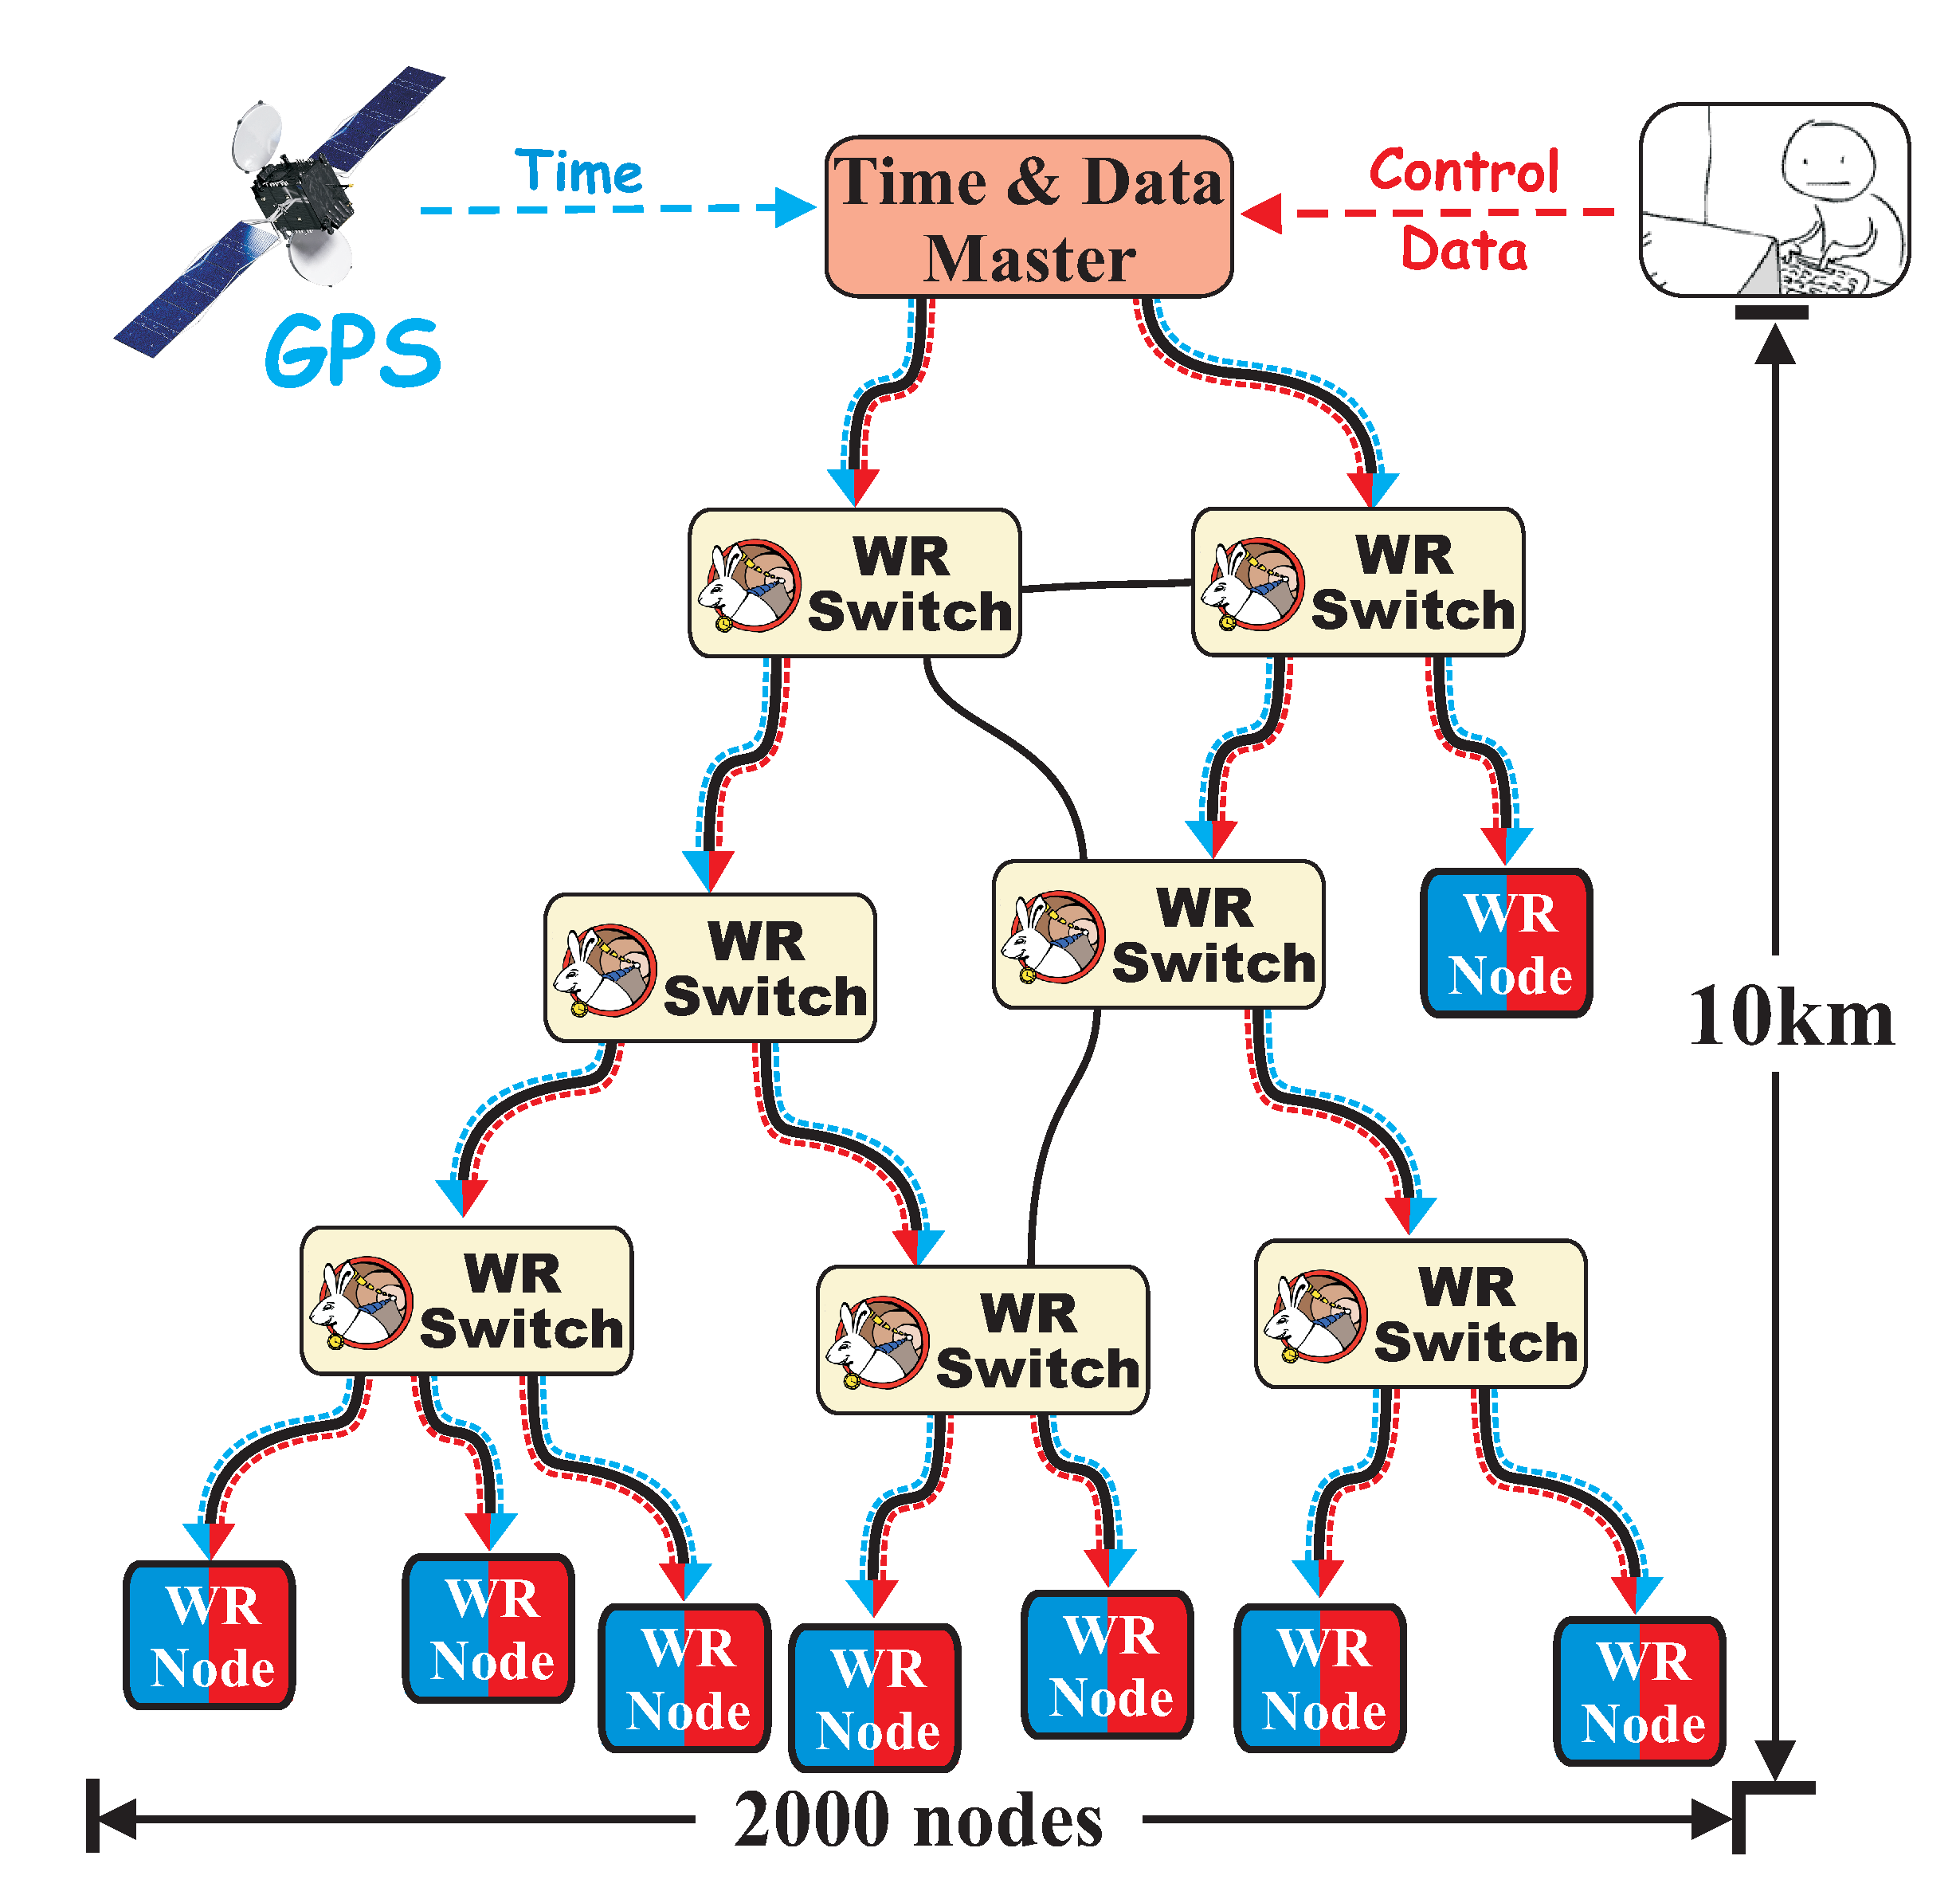
\includegraphics[height=1.0\textwidth]{../../figures/network/wr_network-new.ps}
    \end{center}
\end{columns}

\end{frame}
%%%%%%%%%%%%%%%%%%%%%%%%%%%%%%%%%%%%%%%%%%%%%%%%%%%%%%%%%%%%%%%%%%%%%%%%%%%%%%%%%%%%%%%%%%%%%%%%%%%%
% \section{}
% \subsection{}
%%%%%%%%%%%%%%%%%%%%%%%%%%%%%%%%%%%%%%%%%%%%%%%%%%%%%%%%%%%%%%%%%%%%%%%%%%%%%%%%%%%%%%%%%%%%%%%%%%%%
\begin{frame}{Time Distribution in White Rabbit Network}

  \begin{itemize}
    \item Synchronization with {\bf sub-ns} accuracy and {\bf ps} precision
    \item Combination of
	\begin{itemize}
	  \item Precision Time Protocol ({\bf PTP}) synchronization
	  \item Synchronous Ethernet ({\bf SyncE}) syntonization
	  \item Digital Dual-Mixer Time Difference ({\bf DDMTD}) phase detection
	\end{itemize}
  \end{itemize}
%     \begin{center}
%       \includegraphics[width=1.0\textwidth]{fig/phase_tracking.eps}
%     \end{center}
\end{frame}
%%%%%%%%%%%%%%%%%%%%%%%%%%%%%%%%%%%%%%%%%%%%%%%%%%%%%%%%%%%%%%%%%%%%%%%%%%%%%%%%%%%%%%%%%%%%%%%%%%%%
% \section{}
% \subsection{}
%%%%%%%%%%%%%%%%%%%%%%%%%%%%%%%%%%%%%%%%%%%%%%%%%%%%%%%%%%%%%%%%%%%%%%%%%%%%%%%%%%%%%%%%%%%%%%%%%%%%
\begin{frame}{Precision Time Protocol (IEEE1588)}

\begin{columns}[c]
  \column{1.5in}
      \begin{center}
	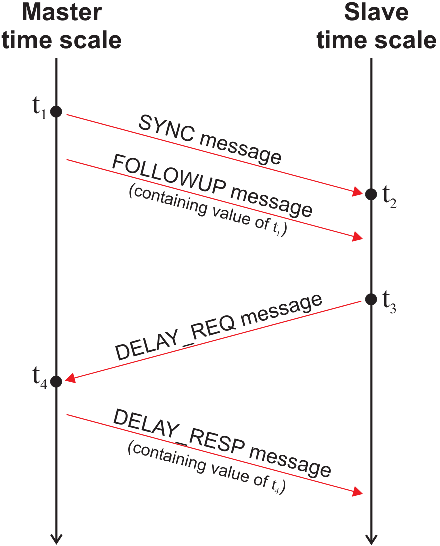
\includegraphics[height=5cm]{../../figures/protocol/ptp_exchange.eps}
      \end{center}
  \column{2.5in}
      \begin{itemize}
	  \item Packet-based synchronization protocol
	  \item Synchronizes local clock with the master clock
	  \item Link delay evaluated by measuring and exchanging packets tx/rx timestamps
      \end{itemize}
  \end{columns}
\end{frame}

%%%%%%%%%%%%%%%%%%%%%%%%%%%%%%%%%%%%%%%%%%%%%%%%%%%%%%%%%%%%%%%%%%%%%%%%%%%%%%%%%%%%%%%%%%%%%%%%%%%%
% \section{}
% \subsection{}
%%%%%%%%%%%%%%%%%%%%%%%%%%%%%%%%%%%%%%%%%%%%%%%%%%%%%%%%%%%%%%%%%%%%%%%%%%%%%%%%%%%%%%%%%%%%%%%%%%%%
\begin{frame}{Synchronous Ethernet (SyncE)}

 \begin{block}{Common clock for the entire network}
%    \textbf{Common clock for the entire network}
    \begin{itemize}
	 \item All network devices use the same physical layer clock
	 \item Clock is encoded in the Ethernet carrier and recovered by the receiver chip (PHY).
    \end{itemize}
\end{block}

\vspace{-0.2cm}

\begin{center}
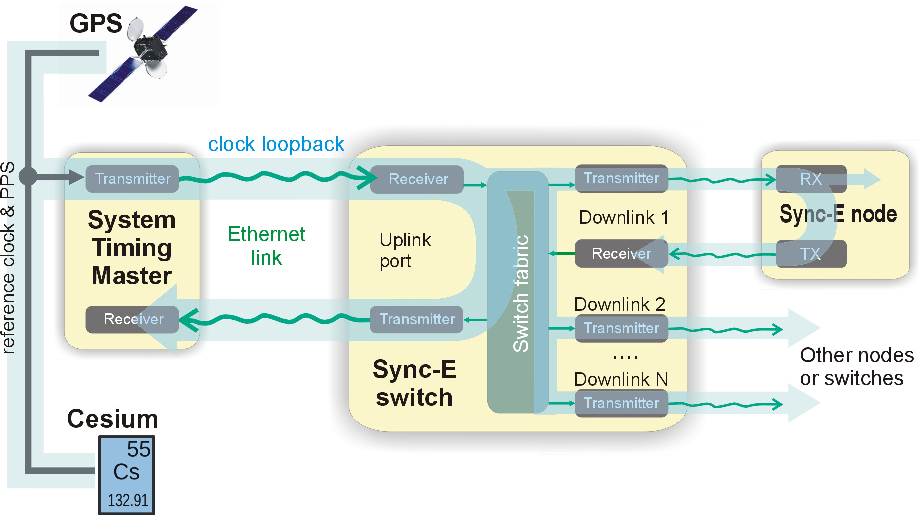
\includegraphics[height=5cm]{../../figures/misc/synce.eps}
\end{center}

\end{frame}
%%%%%%%%%%%%%%%%%%%%%%%%%%%%%%%%%%%%%%%%%%%%%%%%%%%%%%%%%%%%%%%%%%%%%%%%%%%%%%%%%%%%%%%%%%%%%%%%%%%%
% \section{}
% \subsection{}
%%%%%%%%%%%%%%%%%%%%%%%%%%%%%%%%%%%%%%%%%%%%%%%%%%%%%%%%%%%%%%%%%%%%%%%%%%%%%%%%%%%%%%%%%%%%%%%%%%%%
\begin{frame}{DDMTD: Phase tracking}

\small
    \begin{itemize}
      \item PTP limitation: timestamping granularity
      \item Solution: take advantage of SyncE and measure phase shift
    \end{itemize}

  \begin{center}
  \includegraphics[height=2.7cm]{../../figures/misc/phase_tracking.eps}
  \end{center}

\end{frame}

%%%%%%%%%%%%%%%%%%%%%%%%%%%%%%%%%%%%%%%%%%%%%%%%%%%%%%%%%%%%%%%%%%%%%%%%%%%%%%%%%%%%%%%%%%%%%%%%%%%%
% \section{}
% \subsection{}
%%%%%%%%%%%%%%%%%%%%%%%%%%%%%%%%%%%%%%%%%%%%%%%%%%%%%%%%%%%%%%%%%%%%%%%%%%%%%%%%%%%%%%%%%%%%%%%%%%%%
\begin{frame}{WR PTP}

  \begin{itemize}
    \item Extension to PTP (IEEE1588) -- defined as PTP Profile
    \item Addresses PTP's limitations \\(granularity, asymmetry, syntonization)
    \item Compatible with "standard" PTP gear
    \item Ongoing standardization effort (IEEE, ITU-T)
    \item Lab\&field-tested for sub-ns synchronization
  \end{itemize}
  \pause
  \begin{block}{According to ISPCS Plug Fest results ...}
    \begin{center}
      \textbf{... White Rabbit is the most accurate PTP implementation in the world!}
  \end{center}
  \end{block}

\end{frame}
%%%%%%%%%%%%%%%%%%%%%%%%%%%%%%%%%%%%%%%%%%%%%%%%%%%%%%%%%%%%%%%%%%%%%%%%%%%%%%%%%%%%%%%%%%%%%%%%%%%%
%\section{Status}
%\subsection{}
%%%%%%%%%%%%%%%%%%%%%%%%%%%%%%%%%%%%%%%%%%%%%%%%%%%%%%%%%%%%%%%%%%%%%%%%%%%%%%%%%%%%%%%%%%%%%%%%%%%%
\begin{frame}{WR performance}

    \begin{center}
    \includegraphics<1>[height=7.0cm]{../../figures/measurements/measSystem.ps}   \pause
    \includegraphics<2>[height=6.0cm]{../../figures/measurements/measResults-new.eps}
    \end{center}

\end{frame}

%%%%%%%%%%%%%%%%%%%%%%%%%%%%%%%%%%%%%%%%%%%%%%%%%%%%%%%%%%%%%%%%%%%%%%%%%%%%%%%%%%%%%%%%%%%%%%%%%%%%
\section{Data Distribution}
\subsection{}
%%%%%%%%%%%%%%%%%%%%%%%%%%%%%%%%%%%%%%%%%%%%%%%%%%%%%%%%%%%%%%%%%%%%%%%%%%%%%%%%%%%%%%%%%%%%%%%%%%%%
\begin{frame}{Data distribution in White Rabbit}


\begin{columns}[c]
  \column{.47\textwidth}
 
  \begin{itemize}
    \item \color{gray}{High accuracy/precision synchronization}
    \item \textbf{\color{red}{Deterministic, reliable and low-latency Control Data delivery}}
  \end{itemize}

  \column{.6\textwidth}
    \begin{center}
    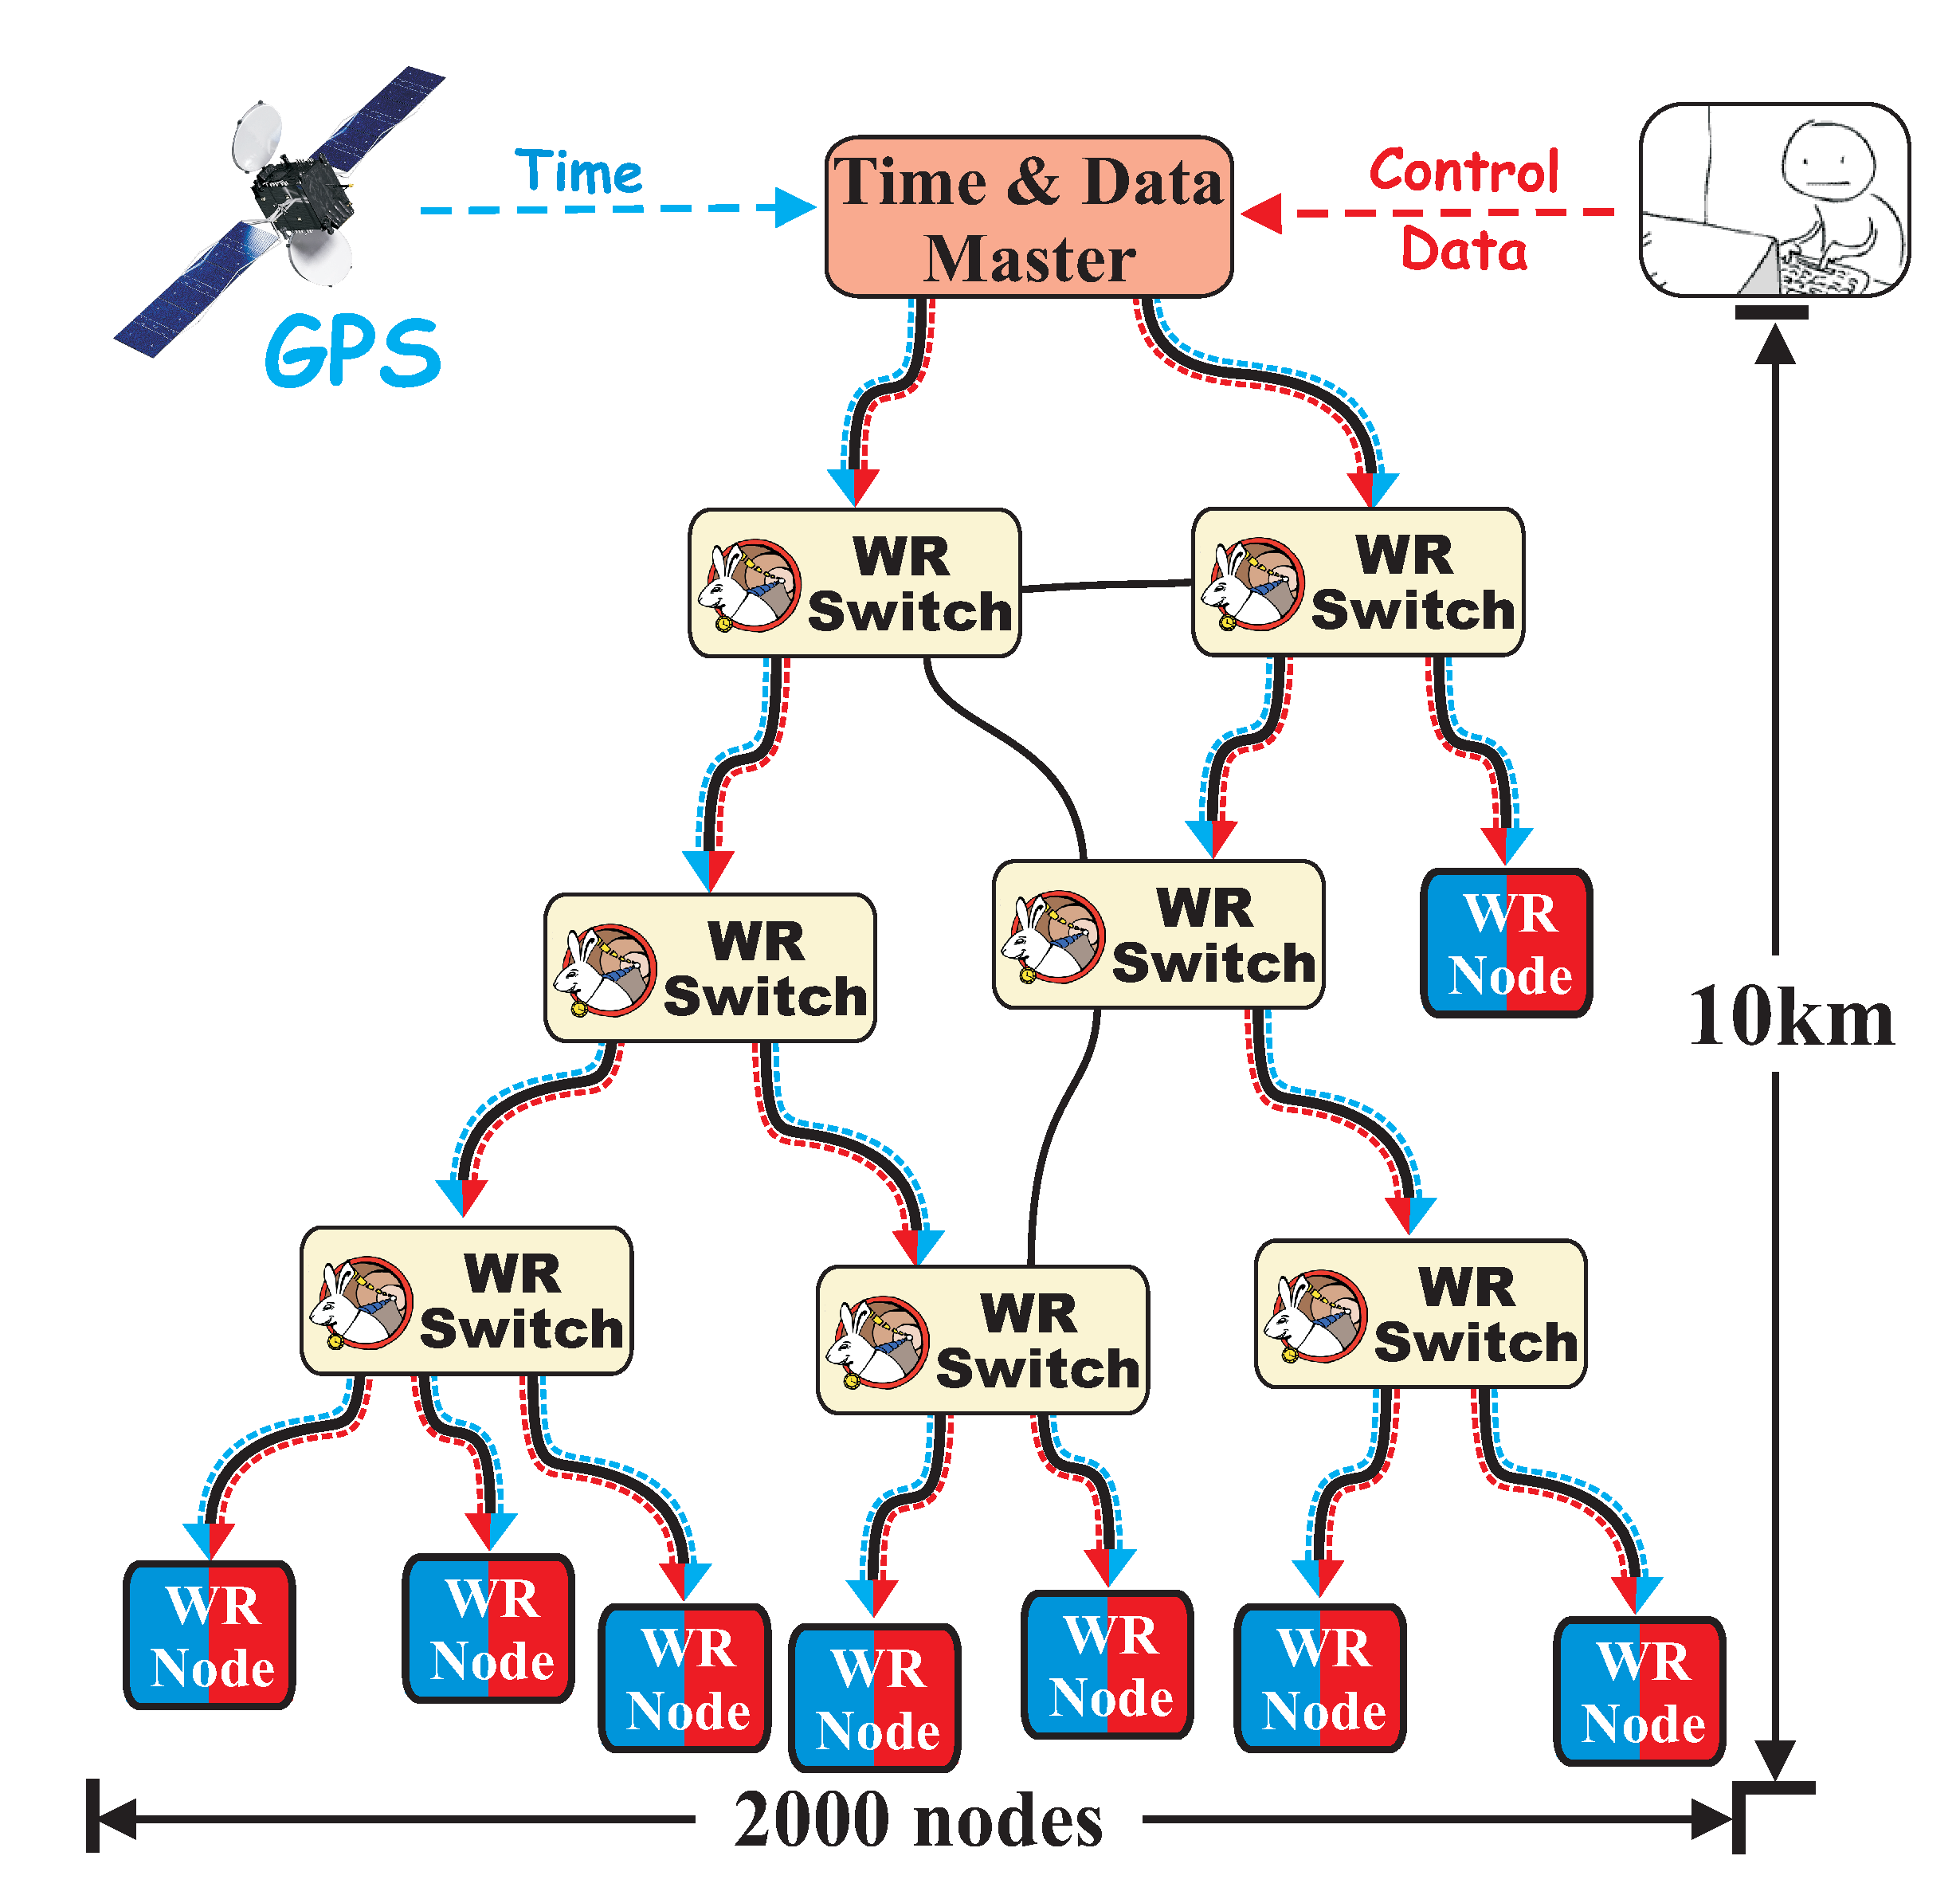
\includegraphics[height=1.0\textwidth]{../../figures/network/wr_network-new.ps}
    \end{center}
\end{columns}

\end{frame}
%%%%%%%%%%%%%%%%%%%%%%%%%%%%%%%%%%%%%%%%%%%%%%%%%%%%%%%%%%%%%%%%%%%%%%%%%%%%%%%%%%%%%%%%%%%%%%%%%%%%
%\section{Status}
%\subsection{}
%%%%%%%%%%%%%%%%%%%%%%%%%%%%%%%%%%%%%%%%%%%%%%%%%%%%%%%%%%%%%%%%%%%%%%%%%%%%%%%%%%%%%%%%%%%%%%%%%%%%
\begin{frame}{Data distribution in WR Control System}

    \begin{center}
    \includegraphics<1>[width=1.1\textwidth]{../../figures/applications/CERN/WRControlNetwork.ps} \pause
    \includegraphics<2>[width=1.1\textwidth]{../../figures/applications/CERN/WRControlNetwork2.ps}
    \end{center}


\end{frame}
%%%%%%%%%%%%%%%%%%%%%%%%%%%%%%%%%%%%%%%%%%%%%%%%%%%%%%%%%%%%%%%%%%%%%%%%%%%%%%%%%%%%%%%%%%%%%%%%%%%%
%\section{Status}
%\subsection{}
%%%%%%%%%%%%%%%%%%%%%%%%%%%%%%%%%%%%%%%%%%%%%%%%%%%%%%%%%%%%%%%%%%%%%%%%%%%%%%%%%%%%%%%%%%%%%%%%%%%%
\begin{frame}{Control Data}

\begin{columns}[c]
  \column{.62\textwidth}
    \begin{itemize}
      \item Two types of data:
	  \begin{itemize}
	    \item \textcolor{red}{\bf Control Data} (High Priority, HP)
	    \item Standard Data (Best Effort)
	  \end{itemize}
	  \item Characteristics of \textcolor{red}{\bf Control Data}
	  \begin{itemize}
	    \item Sent in Control Messages
	    \item Sent by Data Master(s)
	    \item Broadcast (one-to-alot)
	    \item Deterministic and low latency
	    \item Reliable delivery
	  \end{itemize}
    \end{itemize}
  \column{.6\textwidth}
   % \vspace{-1cm}
   % \hspace{-6cm}
    \begin{center}
    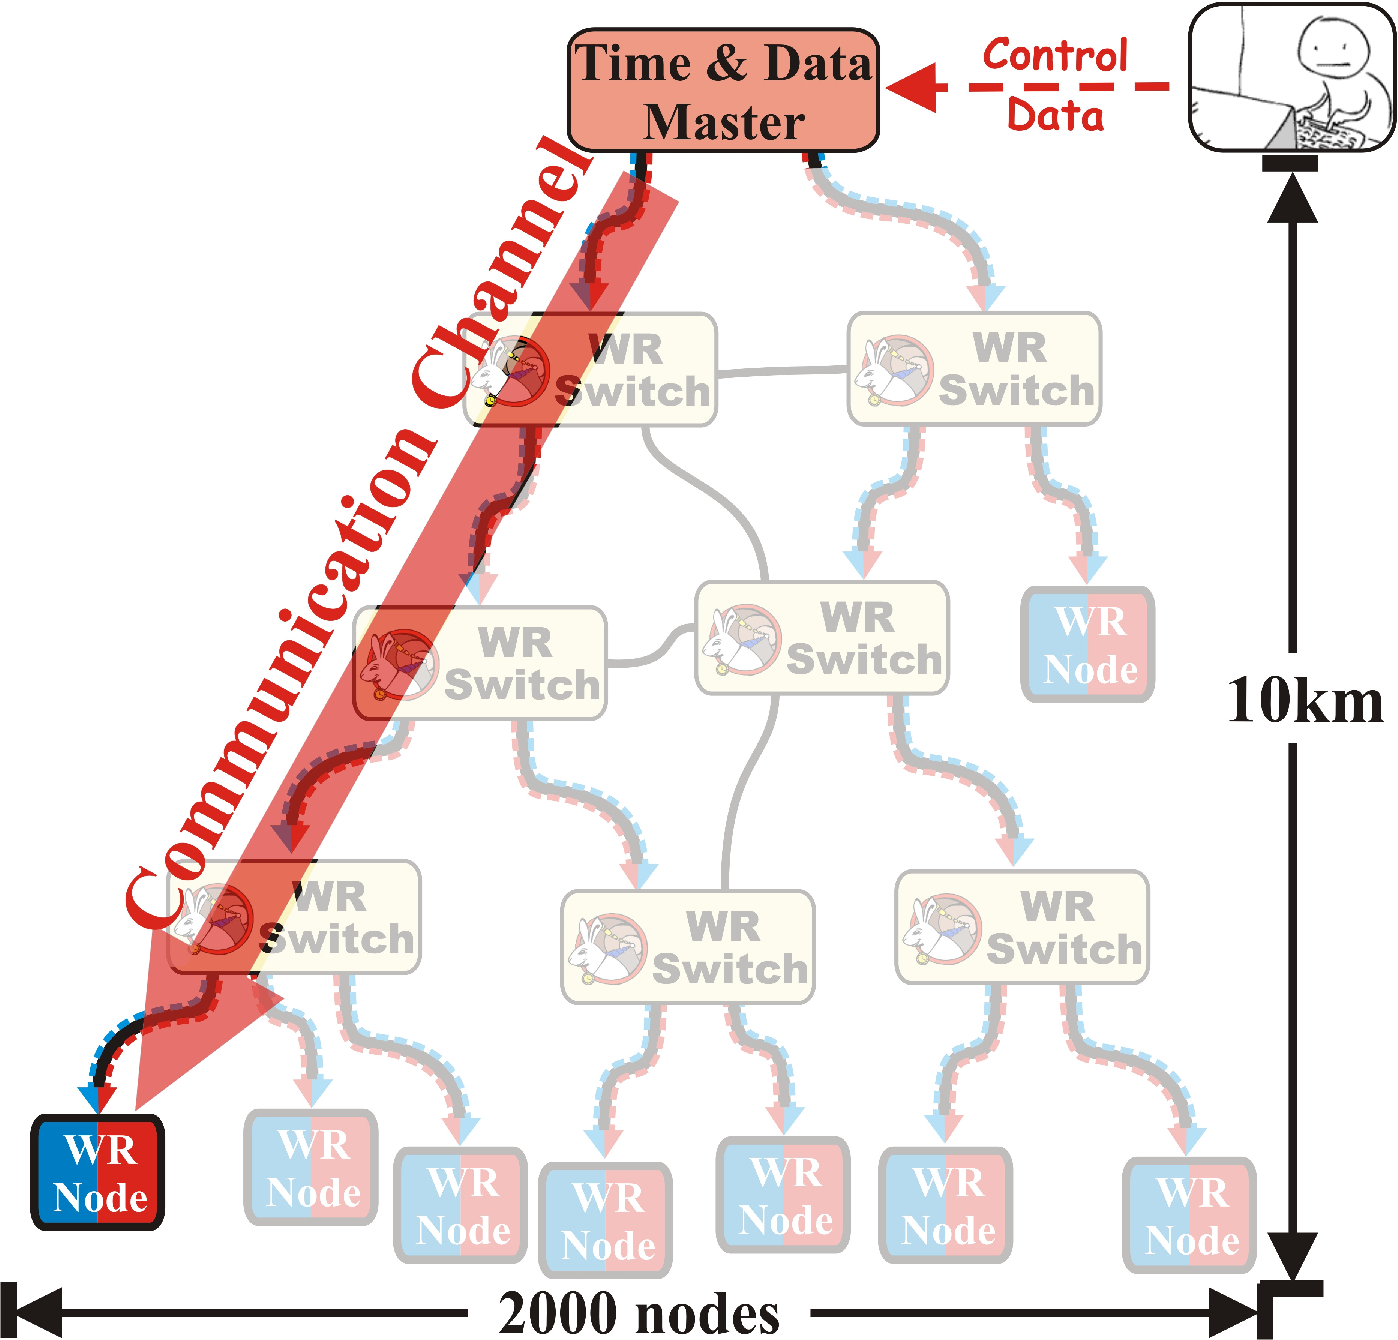
\includegraphics[height=0.6\textheight]{../../figures/robustness/CommunicationChannel.ps}
    \end{center}

\end{columns}

\end{frame}
%%%%%%%%%%%%%%%%%%%%%%%%%%%%%%%%%%%%%%%%%%%%%%%%%%%%%%%%%%%%%%%%%%%%%%%%%%%%%%%%%%%%%%%%%%%%%%%%%%%%
%\section{}
%\subsection{Data Redundancy}
%%%%%%%%%%%%%%%%%%%%%%%%%%%%%%%%%%%%%%%%%%%%%%%%%%%%%%%%%%%%%%%%%%%%%%%%%%%%%%%%%%%%%%%%%%%%%%%%%%%%
\begin{frame}{Data Redundancy}

  \begin{itemize}
    \item Re-transmission of Control Data not possible
	\item {\bf Forward Error Correction}  -- additional transparent layer:
	\begin{itemize}
		\item One Control Message encoded into N Ethernet frames,
		\item Recovery of Control Message from any M (M$<$N) frames
	\end{itemize}
	\item FEC can prevent data loss due to:
	\begin{itemize}	
		\item {\bf bit error} 
		\item {\bf network reconfiguration}
	\end{itemize}	
  \end{itemize}
  
  	\begin{center}
      
\includegraphics[width=.7\textwidth]{../../figures/robustness/FEC.eps}
    \end{center}
  
\end{frame}
%%%%%%%%%%%%%%%%%%%%%%%%%%%%%%%%%%%%%%%%%%%%%%%%%%%%%%%%%%%%%%%%%%%%%%%%%%%%%%%%%%%%%%%%%%%%%%%%%%%%
%\section{}
%\subsection{Topology Redundancy}
%%%%%%%%%%%%%%%%%%%%%%%%%%%%%%%%%%%%%%%%%%%%%%%%%%%%%%%%%%%%%%%%%%%%%%%%%%%%%%%%%%%%%%%%%%%%%%%%%%%%
\begin{frame}{Topology Redundancy}

\begin{columns}[c]
  \column{0.65\textwidth}

      \begin{itemize}
	    \item Standard Ethernet solution: Rapid/Multi Spanning Tree Protocol
	    \item Reconfiguration time: \textbf{$\approx$ 1s} \\ (best: milliseconds)
	    \item \textbf{1s = $\approx$ 82 000} Ethernet Frames lost
	    \item Solution:
	    \begin{itemize}
		  \item take advantage of FEC
		  \item speed up (R/M)STP$->$\textbf{eRSTP} or
		  \item use multiple paths$->$\textbf{eLACP}
	    \end{itemize}

      \end{itemize}
% 
  \column{0.6\textwidth}
    \begin{center}
    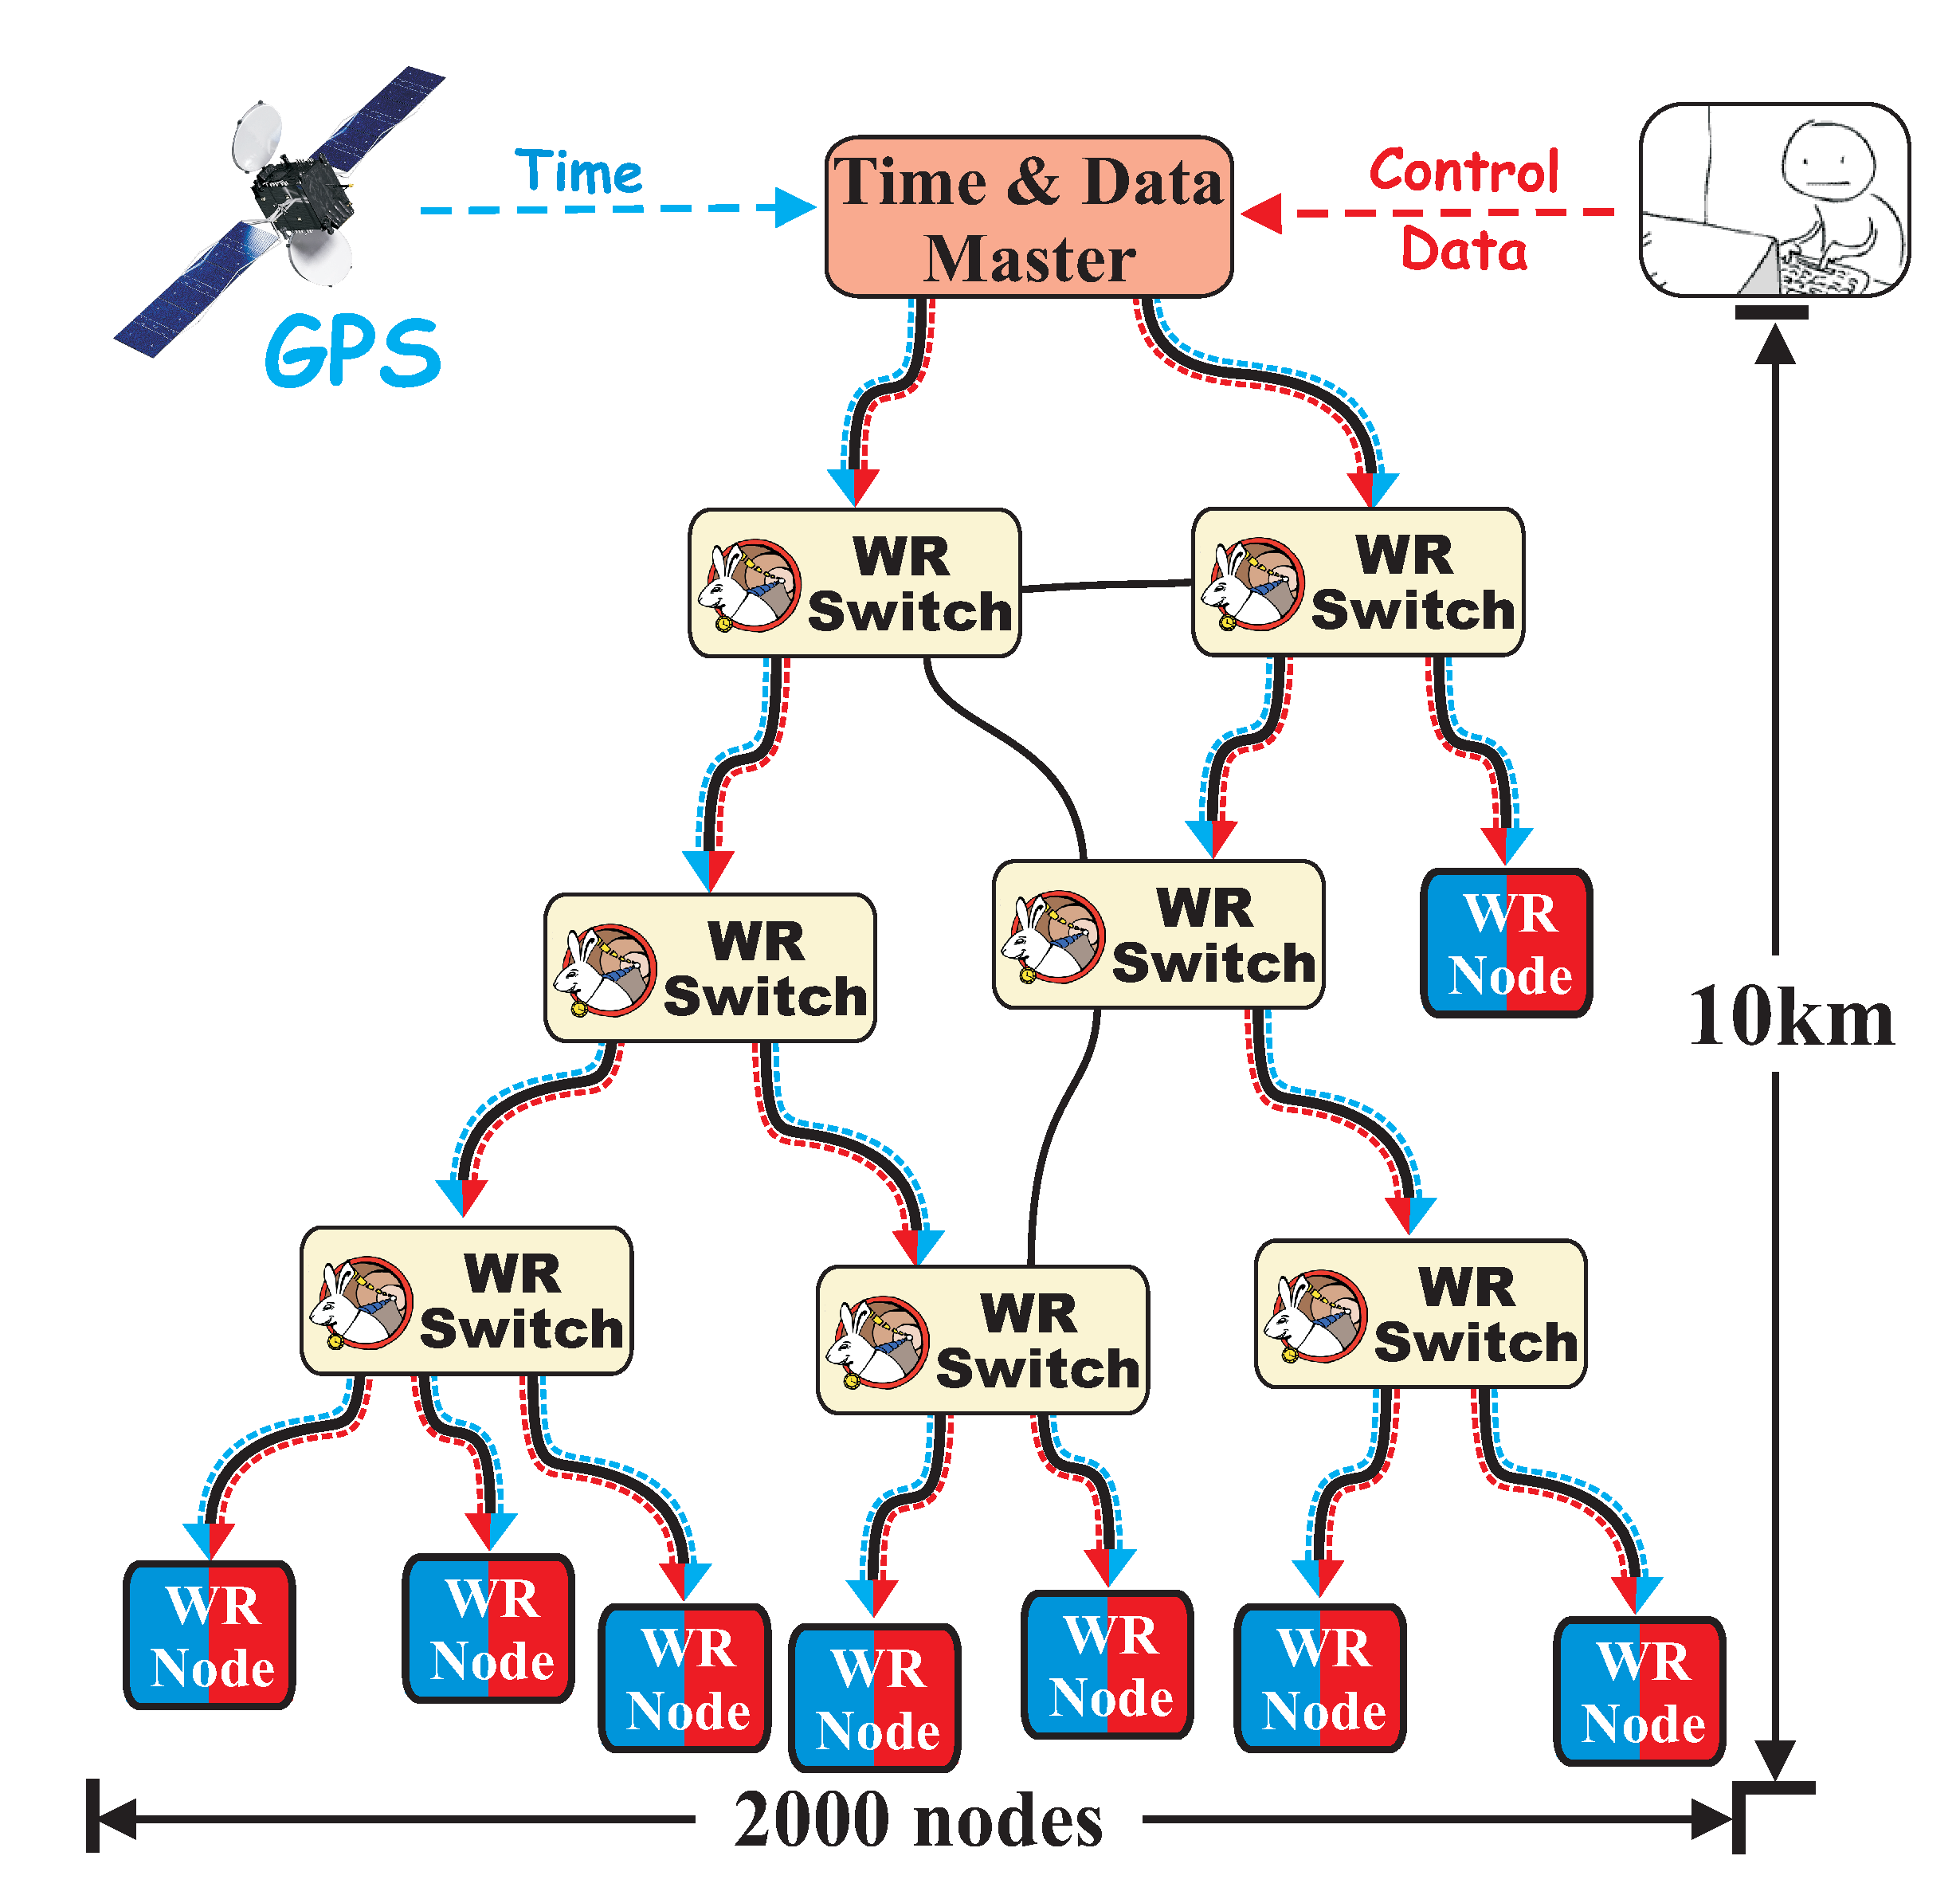
\includegraphics[width=0.65\textwidth]{../../figures/network/wr_network-new.ps}
    \end{center}
\end{columns}

\end{frame}
%%%%%%%%%%%%%%%%%%%%%%%%%%%%%%%%%%%%%%%%%%%%%%%%%%%%%%%%%%%%%%%%%%%%%%%%%%%%%%%%%%%%%%%%%%%%%%%%%%%%
%\section{}
%\subsection{Topology Redundancy}
%%%%%%%%%%%%%%%%%%%%%%%%%%%%%%%%%%%%%%%%%%%%%%%%%%%%%%%%%%%%%%%%%%%%%%%%%%%%%%%%%%%%%%%%%%%%%%%%%%%%
\begin{frame}{Determinism and low latency}

\begin{columns}[c]
  \column{0.6\textwidth}

      \begin{itemize}
	    \item \textcolor{red}{Control Data}: \\$7^{th}$ Class of Service (priority)
	    \item WR Switch:
	    \begin{itemize}
	      \item Quality of Service: resource reservation
	      \item Upper bound latency \\ by design: $<10us$
	      \item Cut-through
	    \end{itemize}
	    \item Careful diagnostics
      \end{itemize}
% 
  \column{0.6\textwidth}
    \begin{center}
    \includegraphics<1>[width=0.65\textwidth]{../../figures/network/wr_network-new.ps} \pause
    \includegraphics<2>[width=0.9\textwidth]{../../figures/robustness/event3.eps} 
    \end{center}

\end{columns}

\end{frame}
%%%%%%%%%%%%%%%%%%%%%%%%%%%%%%%%%%%%%%%%%%%%%%%%%%%%%%%%%%%%%%%%%%%%%%%%%%%%%%%%%%%%%%%%%%%%%%%%%%%%
%\section{}
%\subsection{Topology Redundancy}
%%%%%%%%%%%%%%%%%%%%%%%%%%%%%%%%%%%%%%%%%%%%%%%%%%%%%%%%%%%%%%%%%%%%%%%%%%%%%%%%%%%%%%%%%%%%%%%%%%%%
\begin{frame}{Data Distribution summary}

\small
  \begin{itemize}
    \item Optional feature
    \item Openness enables everyone to verify the parameters
    \item Ongoing efforts (2012/2013)
    \item Commonalities with IEEE effort for $2^{nd}$ gen Audio~Video~Bridging 
  \end{itemize}

\end{frame}
%%%%%%%%%%%%%%%%%%%%%%%%%%%%%%%%%%%%%%%%%%%%%%%%%%%%%%%%%%%%%%%%%%%%%%%%%%%%%%%%%%%%%%%%%%%%%%%%%%%%
\section{System Components}
\subsection{}
%%%%%%%%%%%%%%%%%%%%%%%%%%%%%%%%%%%%%%%%%%%%%%%%%%%%%%%%%%%%%%%%%%%%%%%%%%%%%%%%%%%%%%%%%%%%%%%%%%%%
\begin{frame}{White Rabbit Network Components}


    \begin{center}
    %\includegraphics<1>[width=1.0\textwidth]{fig/WRNcomponents.eps}  \pause
    \includegraphics<1>[width=1.0\textwidth]{../../figures/network/WRnetwork-eva.eps}  \pause
    \includegraphics<2>[width=1.0\textwidth]{../../figures/network/WRNcomponents-1.eps} \pause
    \includegraphics<3>[width=1.0\textwidth]{../../figures/network/WRNcomponents-2.eps}
    \end{center}

\end{frame}
%%%%%%%%%%%%%%%%%%%%%%%%%%%%%%%%%%%%%%%%%%%%%%%%%%%%%%%%%%%%%%%%%%%%%%%%%%%%%%%%%%%%%%%%%%%%%%%%%%%%
%\section{}
%\subsection{Topology Redundancy}
%%%%%%%%%%%%%%%%%%%%%%%%%%%%%%%%%%%%%%%%%%%%%%%%%%%%%%%%%%%%%%%%%%%%%%%%%%%%%%%%%%%%%%%%%%%%%%%%%%%%
\begin{frame}{White Rabbit Switch (V3)}

    \begin{center}
    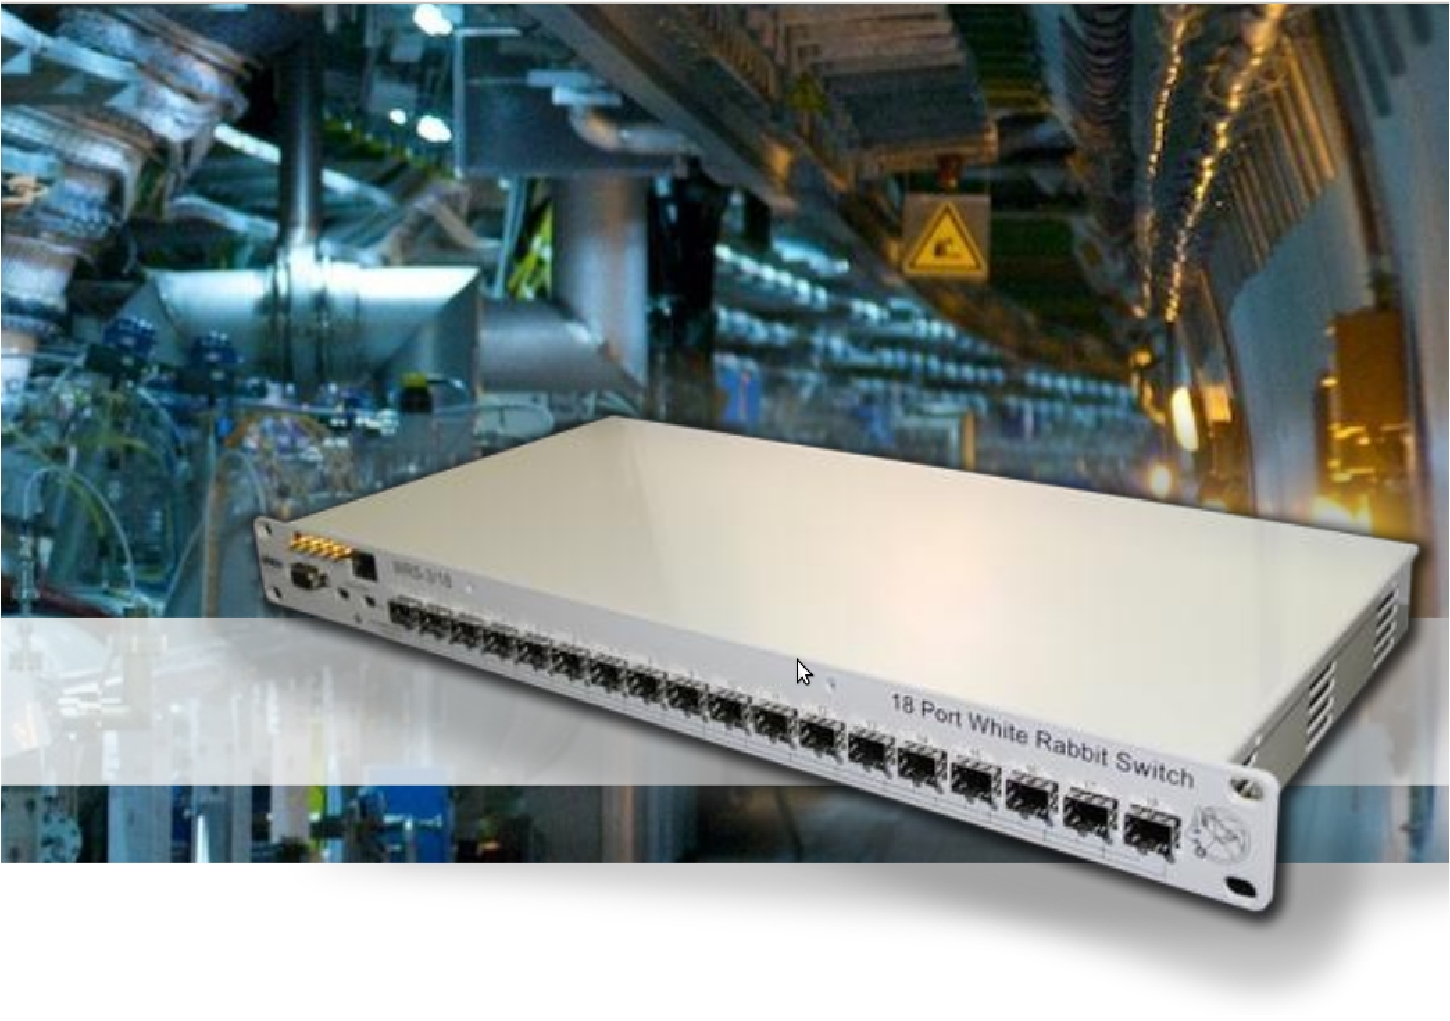
\includegraphics[width=6.0cm]{../../figures/switch/wrSwitchV3.ps}
    \end{center}

	\begin{itemize}
	\item Central element of WR network
	\item Original design optimized for timing, designed from scratch
	\item 18 1000BASE-BX10 ports
	\item Capable of driving 10 km of SM fiber
	\item Open design (H/W and S/W)
%	\item 200 ps synchronization accuracy
	\end{itemize}

\end{frame}
%%%%%%%%%%%%%%%%%%%%%%%%%%%%%%%%%%%%%%%%%%%%%%%%%%%%%%%%%%%%%%%%%%%%%%%%%%%%%%%%%%%%%%%%%%%%%%%%%%%%
%\section{}
%\subsection{Topology Redundancy}
%%%%%%%%%%%%%%%%%%%%%%%%%%%%%%%%%%%%%%%%%%%%%%%%%%%%%%%%%%%%%%%%%%%%%%%%%%%%%%%%%%%%%%%%%%%%%%%%%%%%
\begin{frame}{WR Node: WR PTP Core}

    \begin{center}
    \includegraphics<1>[width=1.0\textwidth]{../../figures/node/wrpc_box.eps} \pause
    \includegraphics<2>[width=1.0\textwidth]{../../figures/node/wrpc_inside.eps}
    \end{center}

\end{frame}
%%%%%%%%%%%%%%%%%%%%%%%%%%%%%%%%%%%%%%%%%%%%%%%%%%%%%%%%%%%%%%%%%%%%%%%%%%%%%%%%%%%%%%%%%%%%%%%%%%%%
%\section{}
%\subsection{Topology Redundancy}
%%%%%%%%%%%%%%%%%%%%%%%%%%%%%%%%%%%%%%%%%%%%%%%%%%%%%%%%%%%%%%%%%%%%%%%%%%%%%%%%%%%%%%%%%%%%%%%%%%%%
\begin{frame}{WR Node: SPEC board}

    \begin{center}
    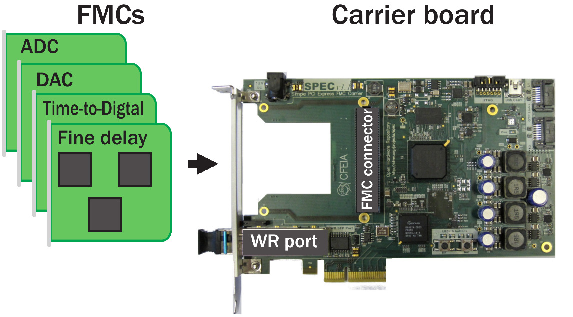
\includegraphics[width=7cm]{../../figures/node/shw_kit-1}
    \end{center}

  \begin{columns}[c]
    \column{.01\textwidth}
    \column{.98\textwidth}

	\begin{block}{Co-HT FMC-based Hardware Kit:}
%	\textbf{Co-HT FMC-based Hardware Kit:}
	  \begin{itemize}
	  \item FMCs (FPGA Mezzanine Cards) with ADCs, DACs, TDCs, fine delays, digital I/O
	  \item Carrier boards in PCI-Express, VME and uTCA formats
	  \item All carriers are equipped with a White Rabbit port
	  \end{itemize}
	\end{block}

    \column{.01\textwidth}
  \end{columns}


\end{frame}

%%%%%%%%%%%%%%%%%%%%%%%%%%%%%%%%%%%%%%%%%%%%%%%%%%%%%%%%%%%%%%%%%%%%%%%%%%%%%%%%%%%%%%%%%%%%%%%%%%%%
%\section{}
%\subsection{Topology Redundancy}
%%%%%%%%%%%%%%%%%%%%%%%%%%%%%%%%%%%%%%%%%%%%%%%%%%%%%%%%%%%%%%%%%%%%%%%%%%%%%%%%%%%%%%%%%%%%%%%%%%%%
\begin{frame}{WR Node: SPEC board}

    \begin{center}
    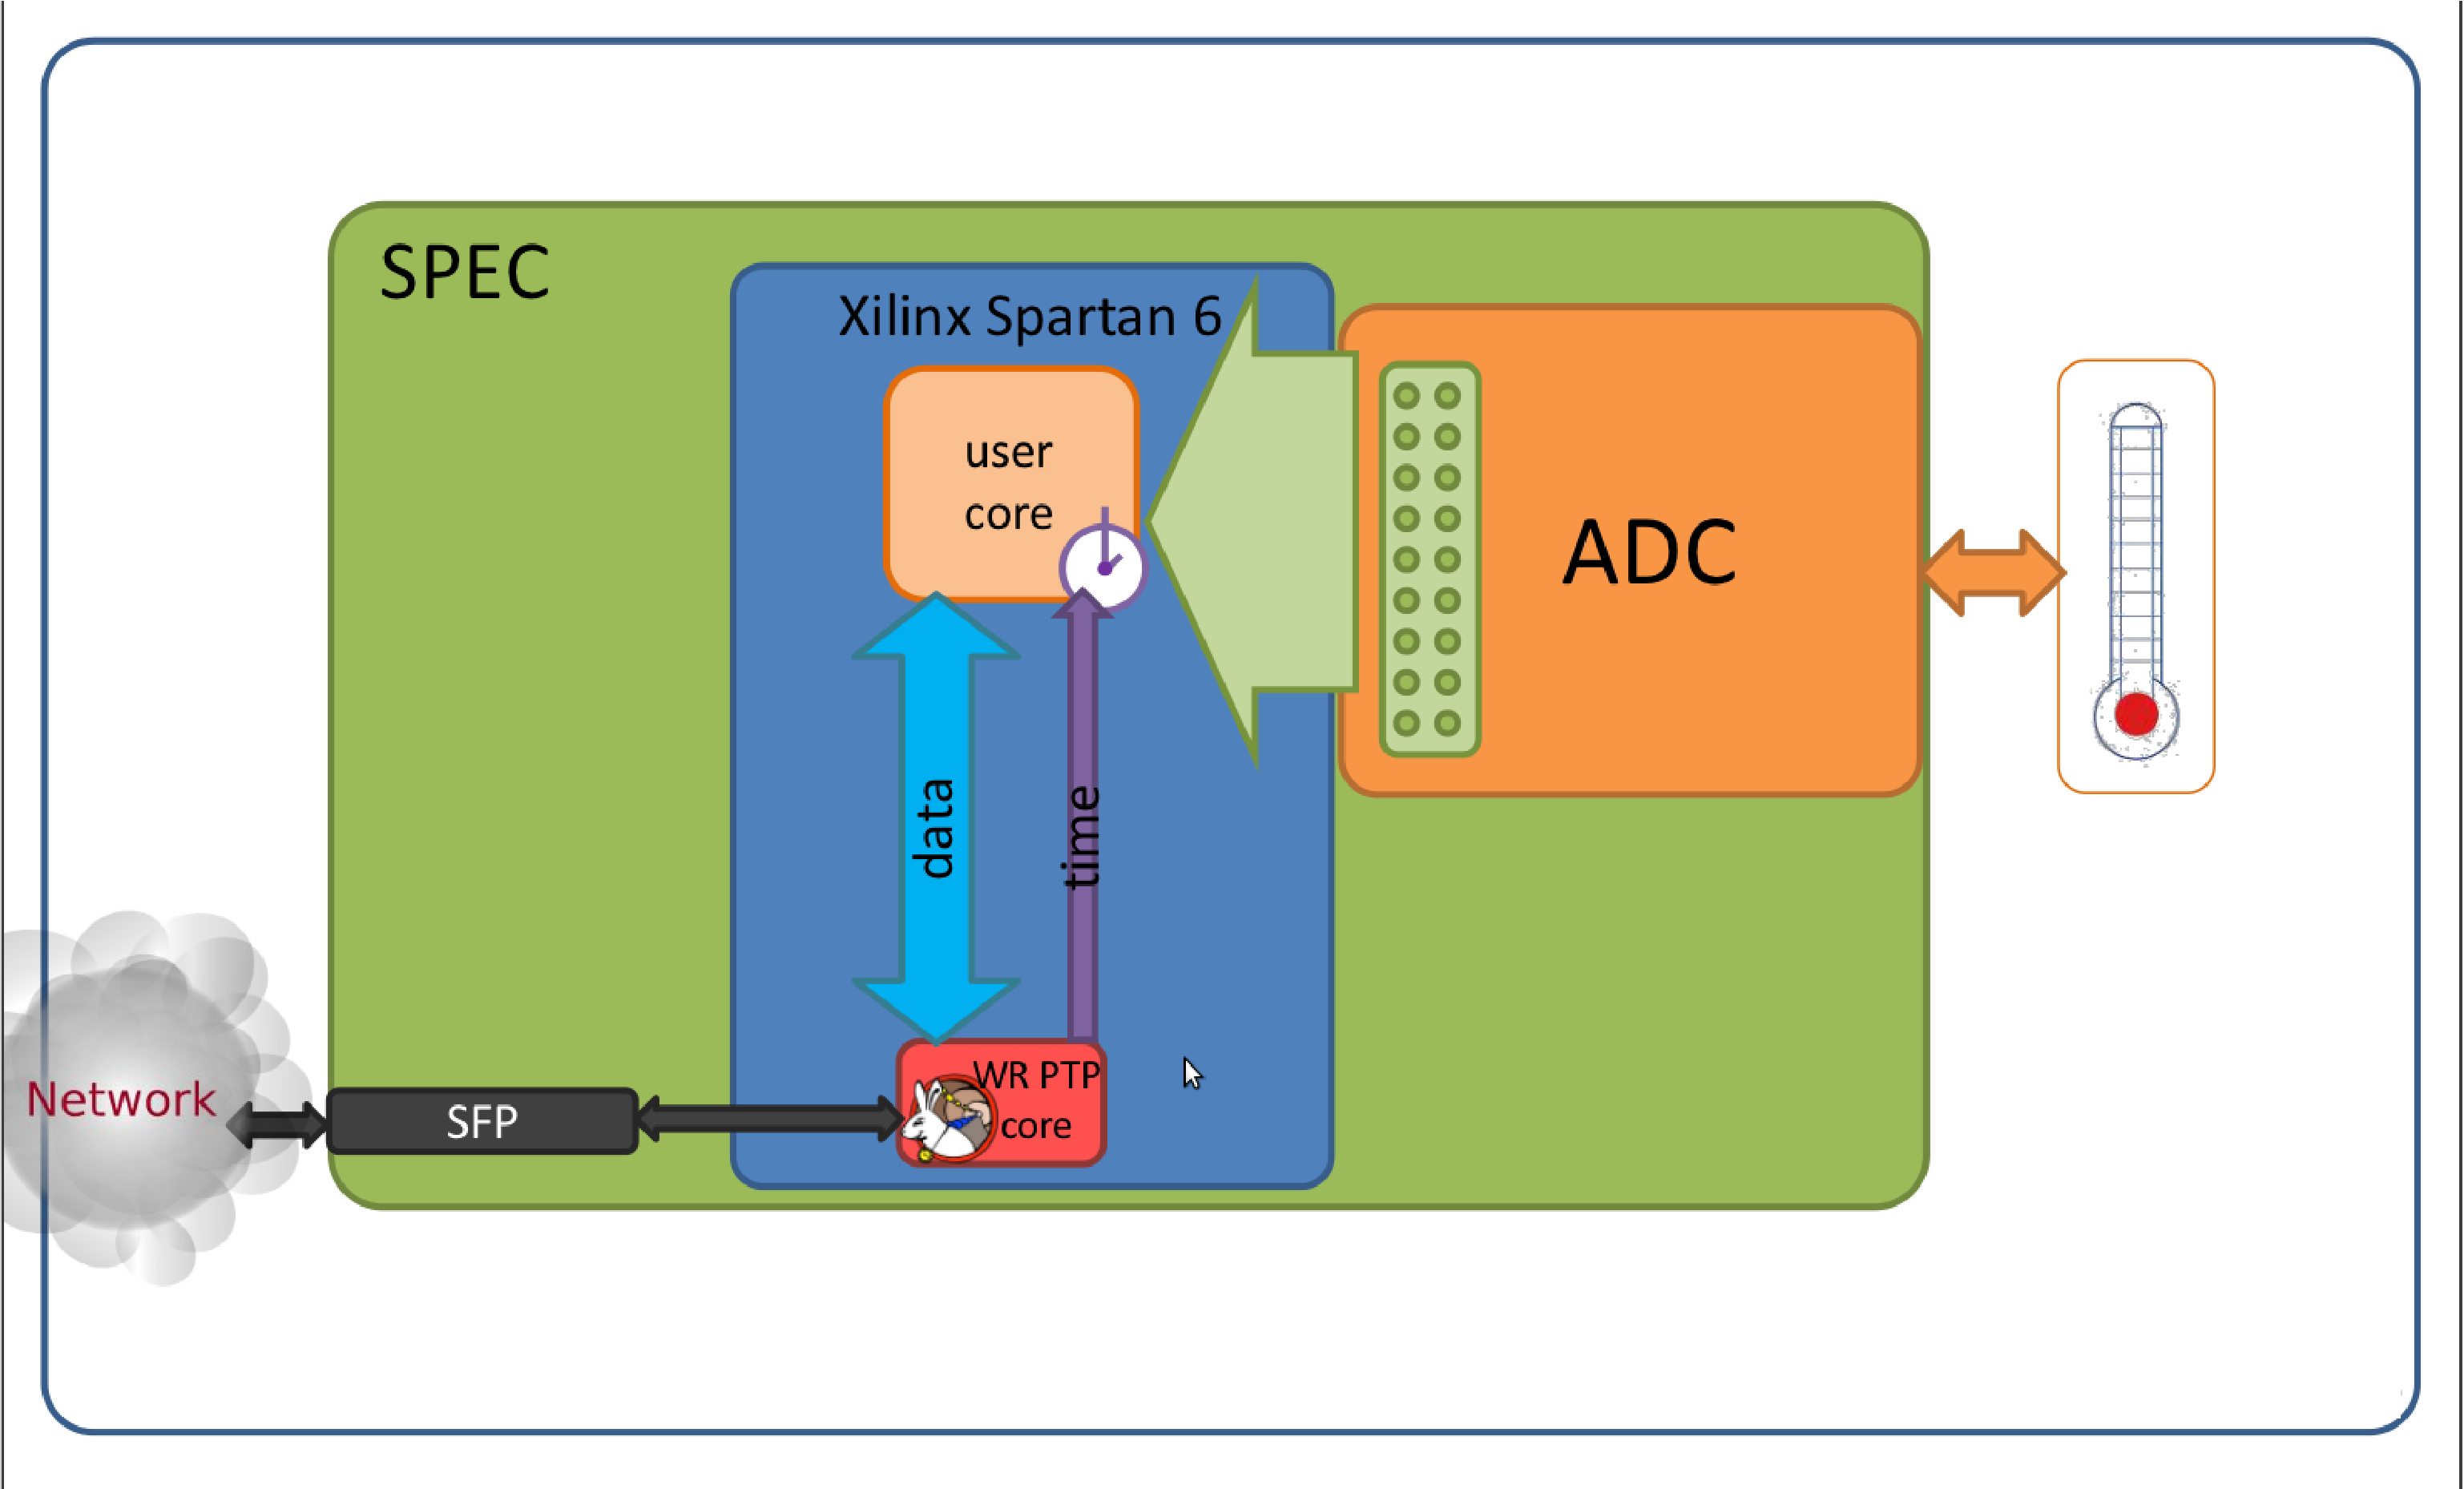
\includegraphics[width=1.0\textwidth]{../../figures/node/specInterior.eps}
    \end{center}

\end{frame}

%%%%%%%%%%%%%%%%%%%%%%%%%%%%%%%%%%%%%%%%%%%%%%%%%%%%%%%%%%%%%%%%%%%%%%%%%%%%%%%%%%%%%%%%%%%%%%%%%%%%
%\section{}
%\subsection{Topology Redundancy}
%%%%%%%%%%%%%%%%%%%%%%%%%%%%%%%%%%%%%%%%%%%%%%%%%%%%%%%%%%%%%%%%%%%%%%%%%%%%%%%%%%%%%%%%%%%%%%%%%%%%
\begin{frame}{WR Node: ongoing efforts}


  \begin{columns}[c]
    \column{.7\textwidth}
\small
      \begin{itemize}
        \item \textbf<1>{Simple VME FMC Carrier (SVEC)}
        \item \textbf<2>{Compact Universal Timing Endpoint Based on White Rabbit}
        \item \textbf<3>{WR-compatible multi-FMC carrier}
	\item \textbf<4>{PXI express FMC Carrier Board (SPEXI)}
      \end{itemize}

    
    \begin{center}
       \textcolor{gray}{www.ohwr.org/projects/spexi/wiki}
    \end{center}


    \column{.5\textwidth}

    \begin{center}
      \includegraphics<1>[width=0.9\textwidth]{../../figures/node/svec4_res.eps} \pause
      \includegraphics<2>[width=0.7\textwidth]{../../figures/node/stm.eps}       \pause
      \includegraphics<3>[width=0.9\textwidth]{../../figures/node/WRCarrier.eps} \pause
      \includegraphics<4>[width=0.5\textwidth]{../../figures/node/pxi.eps} 
    \end{center}

    \column{.01\textwidth}
  \end{columns}

%     \begin{center}
%     \includegraphics<1>[width=1.0\textwidth]{fig/stm.eps}       \pause
%     \includegraphics<2>[width=1.0\textwidth]{fig/svec4_res.eps} \pause
%     \includegraphics<3>[width=1.0\textwidth]{fig/WRCarrier.eps}
%     \end{center}

\end{frame}
%%%%%%%%%%%%%%%%%%%%%%%%%%%%%%%%%%%%%%%%%%%%%%%%%%%%%%%%%%%%%%%%%%%%%%%%%%%%%%%%%%%%%%%%%%%%%%%%%%%%
\section{Applications}
\subsection{}
%%%%%%%%%%%%%%%%%%%%%%%%%%%%%%%%%%%%%%%%%%%%%%%%%%%%%%%%%%%%%%%%%%%%%%%%%%%%%%%%%%%%%%%%%%%%%%%%%%%%
\begin{frame}{White Rabbit applications}

  \begin{itemize}
    \item Control and timing system
    \item Field bus recommended at CERN
    \item Time Transfer
    \item RF distribution
    \item Distributed oscilloscope
    \item ...
  \end{itemize}

\end{frame}
%%%%%%%%%%%%%%%%%%%%%%%%%%%%%%%%%%%%%%%%%%%%%%%%%%%%%%%%%%%%%%%%%%%%%%%%%%%%%%%%%%%%%%%%%%%%%%%%%%%%
% \section{}
% \subsection{}
%%%%%%%%%%%%%%%%%%%%%%%%%%%%%%%%%%%%%%%%%%%%%%%%%%%%%%%%%%%%%%%%%%%%%%%%%%%%%%%%%%%%%%%%%%%%%%%%%%%%
\begin{frame}{WR at CERN}

      \begin{center}
      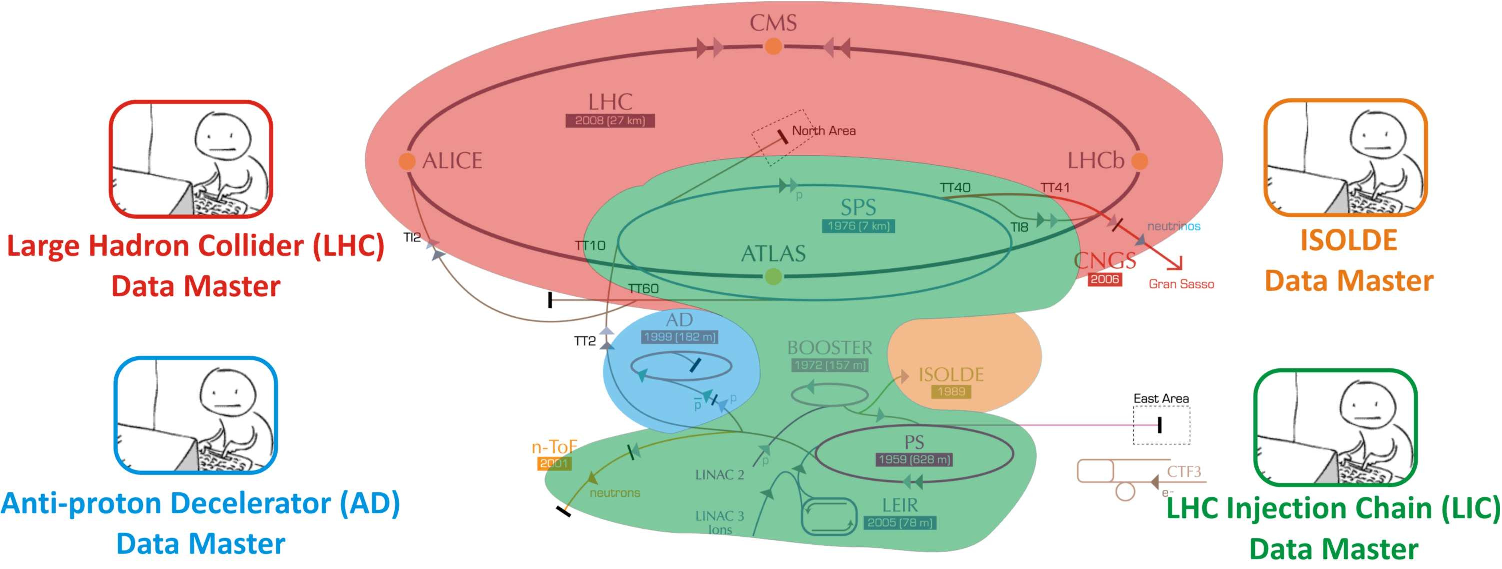
\includegraphics[width=.7\textwidth]{../../figures/applications/CERN/accNetworks.eps}
      \end{center}

  \begin{itemize}
    \item 4 accelerator networks
    \item Separate {\bf Data Master (DM)} for each network
    \item \textcolor{green!90}{LIC Data Master} communicates with other DMs and control devices in their networks
    \item Broadcast of {\bf Control Messages} within network(s)
  \end{itemize}

\end{frame}
%%%%%%%%%%%%%%%%%%%%%%%%%%%%%%%%%%%%%%%%%%%%%%%%%%%%%%%%%%%%%%%%%%%%%%%%%%%%%%%%%%%%%%%%%%%%%%%%%%%%
%\section{WR-based Control System}
%\subsection{}
%%%%%%%%%%%%%%%%%%%%%%%%%%%%%%%%%%%%%%%%%%%%%%%%%%%%%%%%%%%%%%%%%%%%%%%%%%%%%%%%%%%%%%%%%%%%%%%%%%%%
\begin{frame}{WR at CERN}

    \begin{center}
      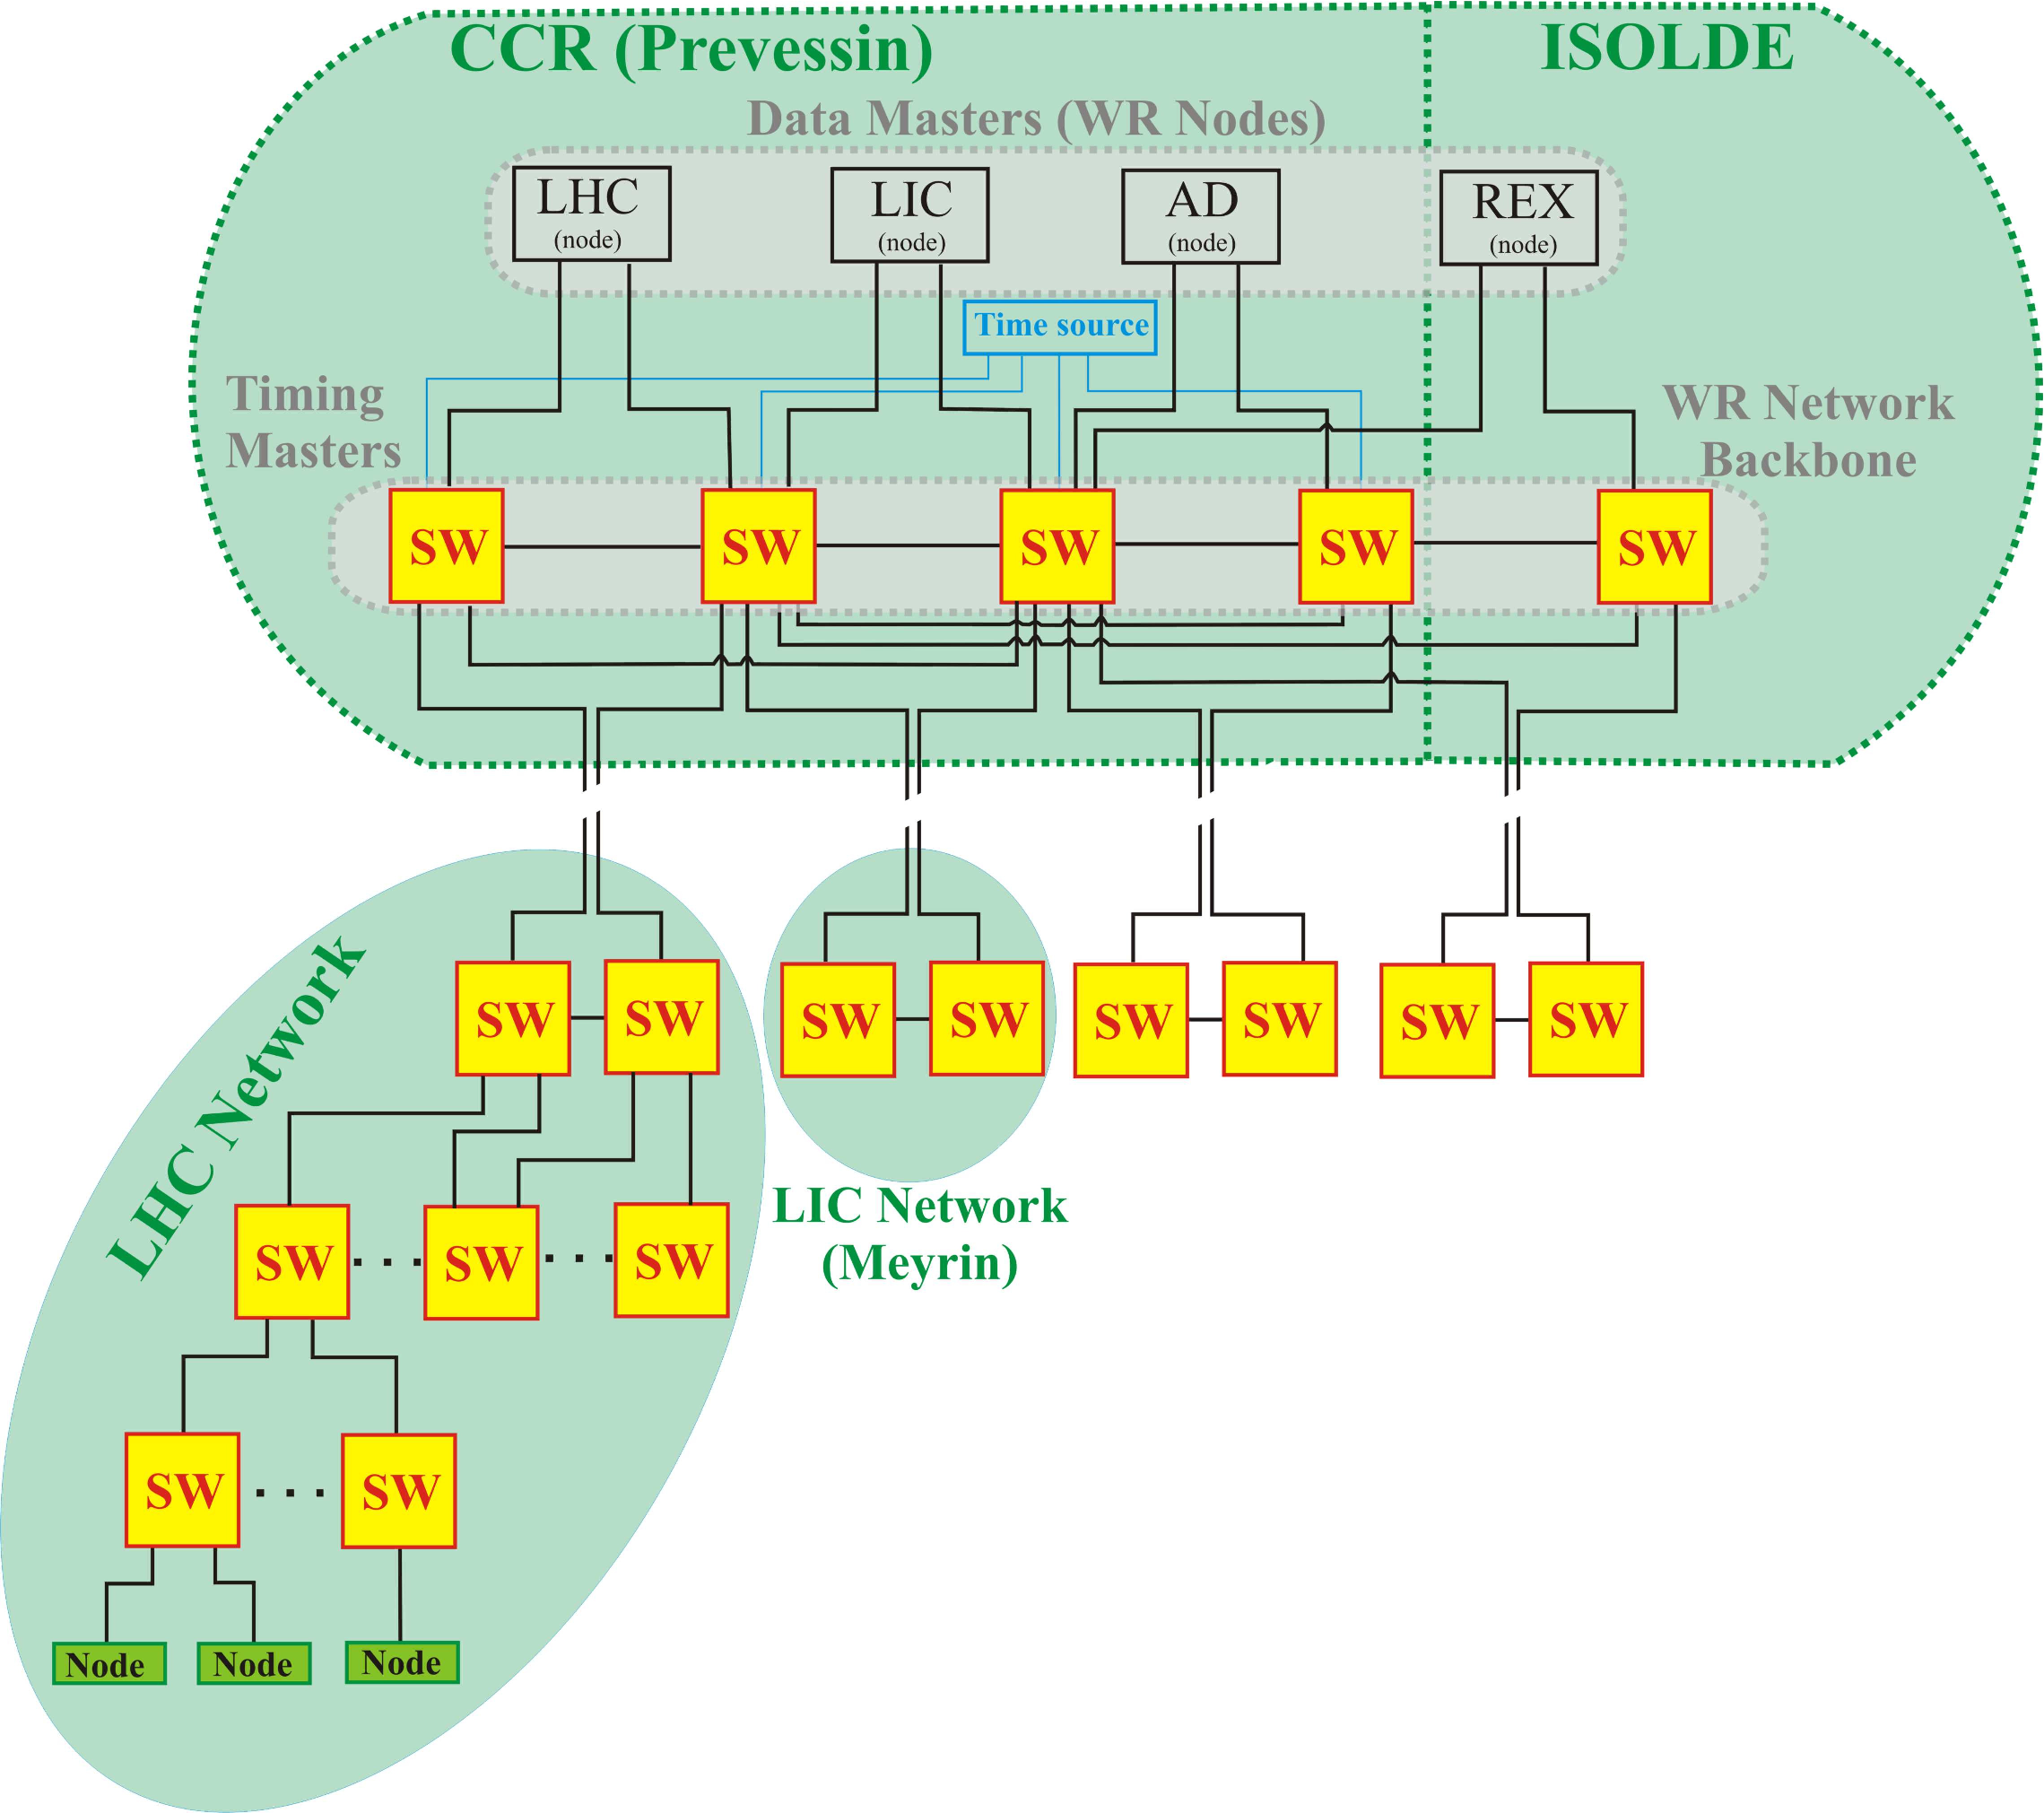
\includegraphics[width=.8\textwidth]{../../figures/applications/CERN/NT-overview.eps}
    \end{center}

\end{frame}
%%%%%%%%%%%%%%%%%%%%%%%%%%%%%%%%%%%%%%%%%%%%%%%%%%%%%%%%%%%%%%%%%%%%%%%%%%%%%%%%%%%%%%%%%%%%%%%%%%%%
%\section{Applications}
%\subsection{Topology Redundancy}
%%%%%%%%%%%%%%%%%%%%%%%%%%%%%%%%%%%%%%%%%%%%%%%%%%%%%%%%%%%%%%%%%%%%%%%%%%%%%%%%%%%%%%%%%%%%%%%%%%%%
\begin{frame}{Ethernet Clock distribution a.k.a. Distributed DDS}
  \begin{center}
    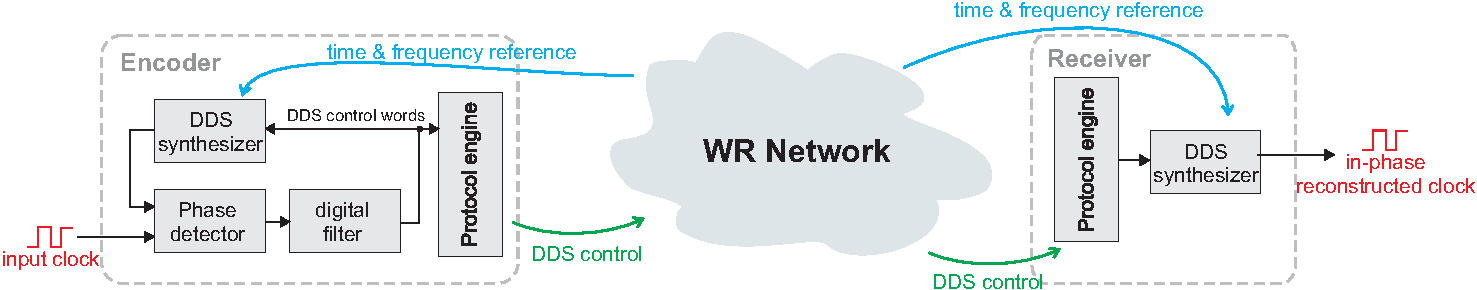
\includegraphics[width=\columnwidth]{../../figures/applications/remote_dds.eps}
  \end{center}
  \begin{block}{Distributed Direct Digital Synthesis}
    \begin{itemize}
    \item Replaces dozens of cables with a single fiber.
    \item Works over big distances without degrading signal quality.
    \item Can provide various clocks (TTC, RF, bunch clock) with a single, standardized link.
    \end{itemize}
  \end{block}
\end{frame}

%%%%%%%%%%%%%%%%%%%%%%%%%%%%%%%%%%%%%%%%%%%%%%%%%%%%%%%%%%%%%%%%%%%%%%%%%%%%%%%%%%%%%%%%%%%%%%%%%%%%
%\section{Applications}
%\subsection{Topology Redundancy}
%%%%%%%%%%%%%%%%%%%%%%%%%%%%%%%%%%%%%%%%%%%%%%%%%%%%%%%%%%%%%%%%%%%%%%%%%%%%%%%%%%%%%%%%%%%%%%%%%%%%
\begin{frame}{Distributed oscilloscope}
  \begin{center}
    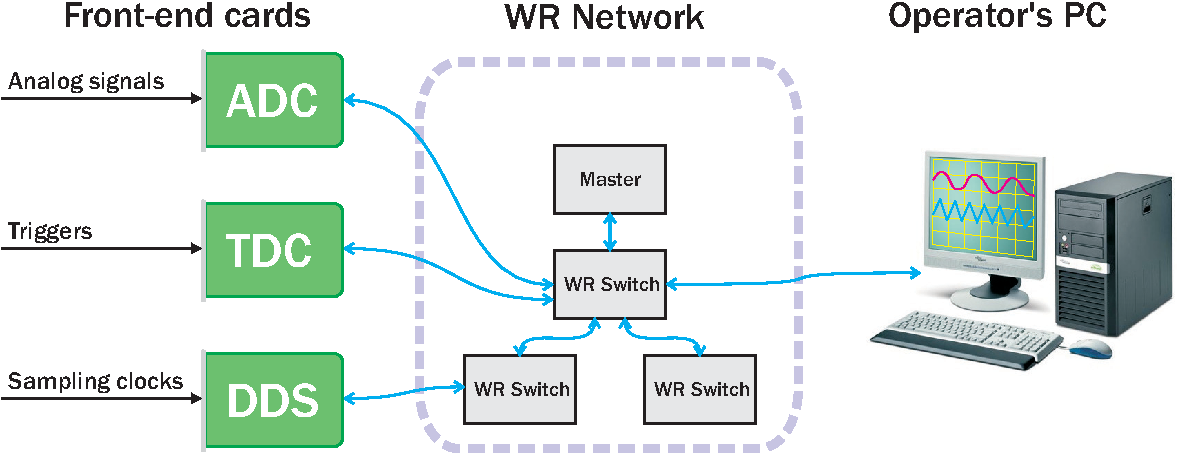
\includegraphics[width=0.9\textwidth]{../../figures/applications/distr_oscill.eps}
    \end{center}
    \begin{block}{}
      \begin{itemize}
      \item Common clock in the entire network: no skew between ADCs.
      \item Ability to sample with different clocks via Distributed DDS.
      \item External triggers can be time tagged with a TDC and used to reconstruct the original time base in the operator's PC.
      \end{itemize}
    \end{block}
\end{frame}
%%%%%%%%%%%%%%%%%%%%%%%%%%%%%%%%%%%%%%%%%%%%%%%%%%%%%%%%%%%%%%%%%%%%%%%%%%%%%%%%%%%%%%%%%%%%%%%%%%%%
%\section{Applications}
%\subsection{Topology Redundancy}
%%%%%%%%%%%%%%%%%%%%%%%%%%%%%%%%%%%%%%%%%%%%%%%%%%%%%%%%%%%%%%%%%%%%%%%%%%%%%%%%%%%%%%%%%%%%%%%%%%%%
\begin{frame}{Time Transfer}
  \begin{columns}[c]
    \column{.7\textwidth}
      \begin{itemize}
	\item WR Network connected to \\ Cs Clock and GPS
	\item SPEC + Fine Delay FMC module
	\begin{itemize}
	  \item Time-to-Digital Converter
	  \begin{itemize}
	    \item 28 ps resolution
	    \item 55ps precision (std.dev)
	    \item 300 ps accuracy (WR-timebase)
	  \end{itemize}
	  \item Pulse Generator:
	  \begin{itemize}
	    \item Produces pulses at UTC/TAI
	    \item Pulse width: 50ns-1s (res: 10ps )
	    \item Pulse spacing: 100ns-1s (res: 10ps)
	  \end{itemize}
	\end{itemize}
      \end{itemize}
    \column{.4\textwidth}
      \begin{center}
	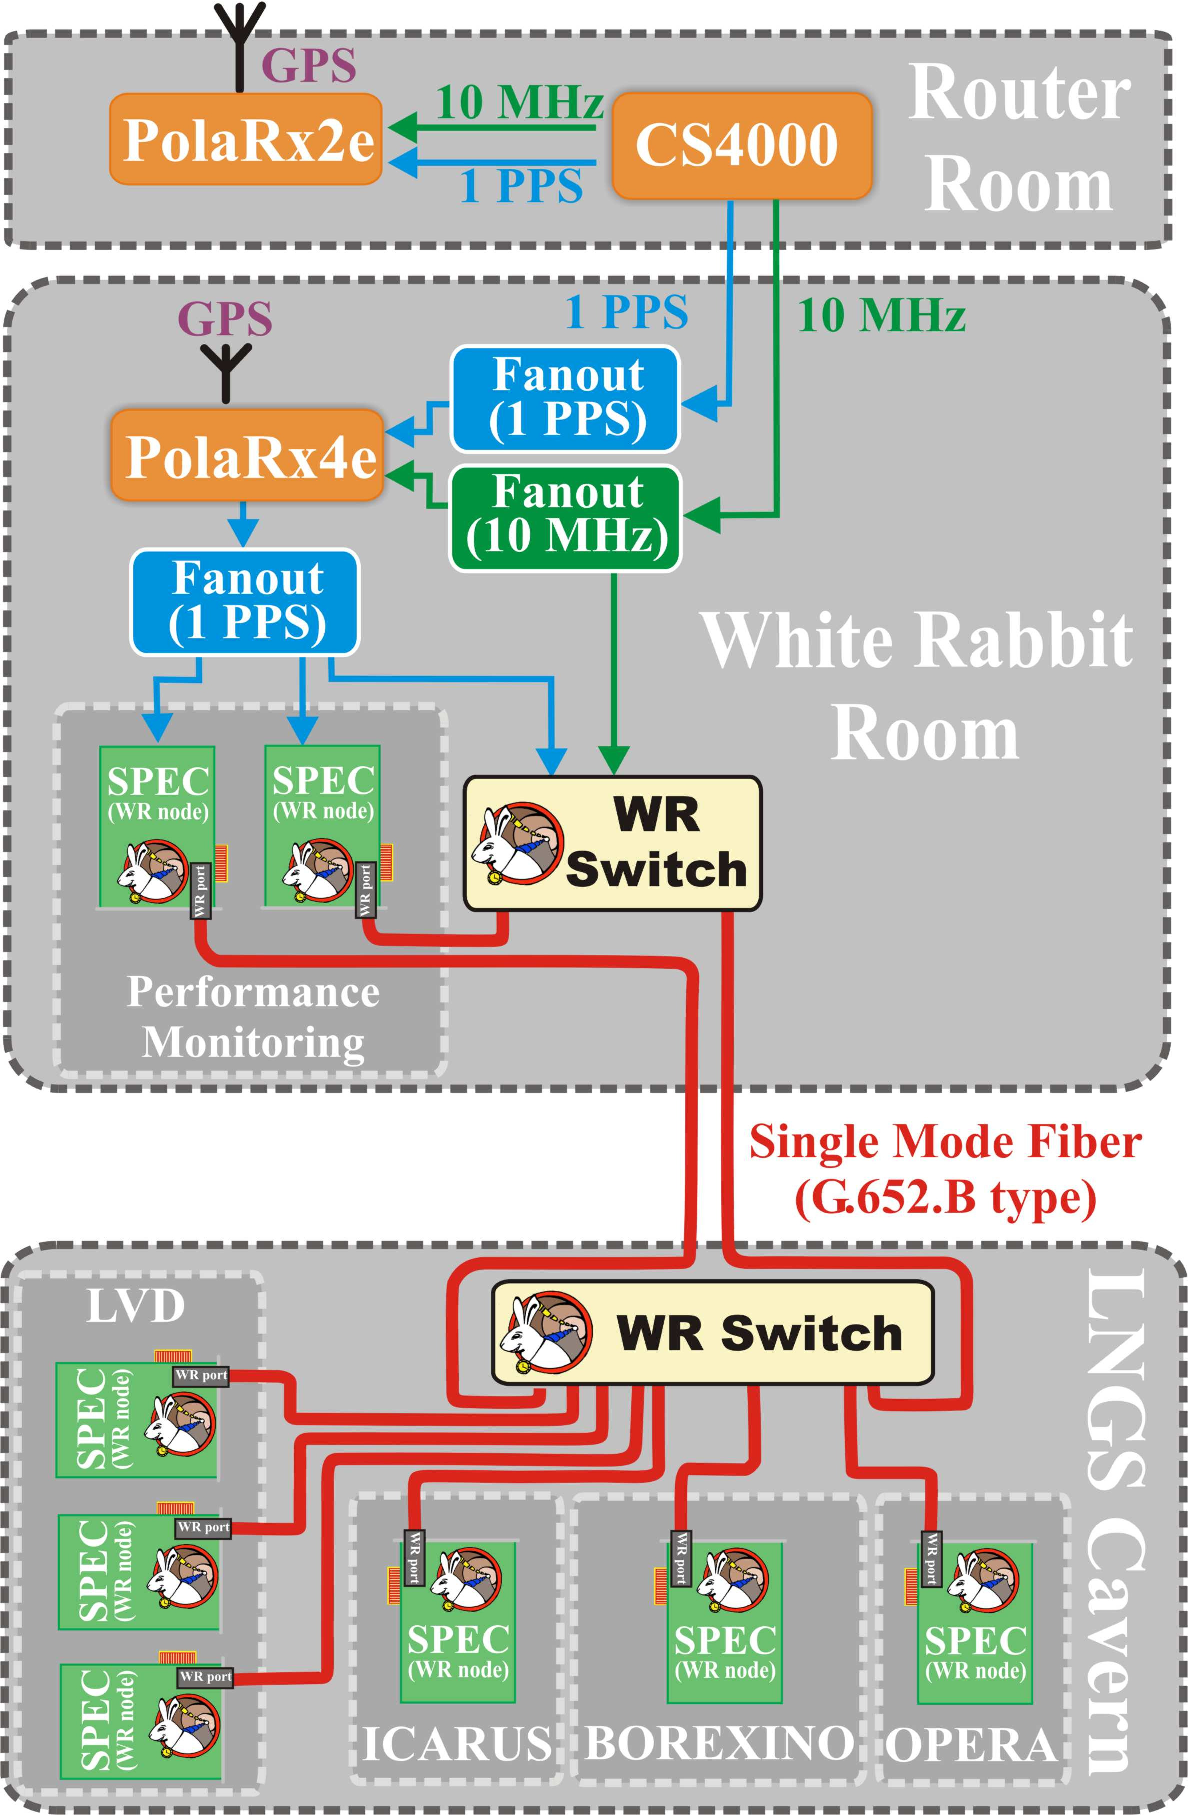
\includegraphics[width=0.9\textwidth]{../../figures/applications/CNGS2.eps}
      \end{center}
    \column{.01\textwidth}
  \end{columns}
\end{frame}
%%%%%%%%%%%%%%%%%%%%%%%%%%%%%%%%%%%%%%%%%%%%%%%%%%%%%%%%%%%%%%%%%%%%%%%%%%%%%%%%%%%%%%%%%%%%%%%%%%%%
%\section{Applications}
%\subsection{Topology Redundancy}
%%%%%%%%%%%%%%%%%%%%%%%%%%%%%%%%%%%%%%%%%%%%%%%%%%%%%%%%%%%%%%%%%%%%%%%%%%%%%%%%%%%%%%%%%%%%%%%%%%%%
\begin{frame}{Time Transfer}

      \begin{center}
	\includegraphics<1>[width=0.9\textwidth]{../../figures/measurements/teAndHist4.eps} \pause
	\includegraphics<2>[width=0.9\textwidth]{../../figures/measurements/MTIE-corrections-long-data.eps}	
      \end{center}

 
\end{frame}
%%%%%%%%%%%%%%%%%%%%%%%%%%%%%%%%%%%%%%%%%%%%%%%%%%%%%%%%%%%%%%%%%%%%%%%%%%%%%%%%%%%%%%%%%%%%%%%%%%%%
%\section{Applications}
%\subsection{Topology Redundancy}
%%%%%%%%%%%%%%%%%%%%%%%%%%%%%%%%%%%%%%%%%%%%%%%%%%%%%%%%%%%%%%%%%%%%%%%%%%%%%%%%%%%%%%%%%%%%%%%%%%%%

\begin{frame}{Beam Position Monitoring}

  \begin{columns}[c]
    \column{.6\textwidth}

      \begin{itemize}
	\item Open Hardware project by Brazilian Light Source
	\item Seriously considering WR for communication among BPM stations
      \end{itemize}

    \begin{center}
      \textcolor{gray}{www.ohwr.org/projects/bpm}
    \end{center}


    \column{.5\textwidth}

    \begin{center}
      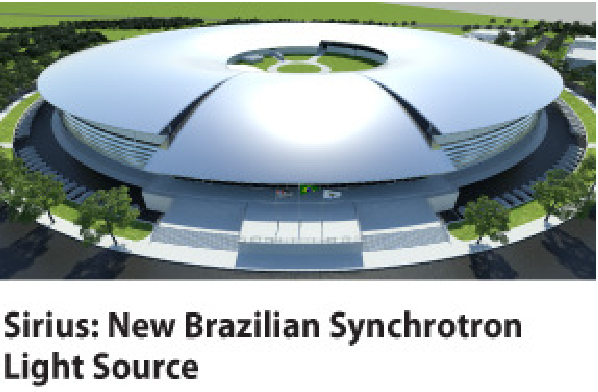
\includegraphics[width=1.0\textwidth]{../../figures/applications/sirius8.eps}
    \end{center}

    \column{.01\textwidth}
  \end{columns}

\end{frame}
%%%%%%%%%%%%%%%%%%%%%%%%%%%%%%%%%%%%%%%%%%%%%%%%%%%%%%%%%%%%%%%%%%%%%%%%%%%%%%%%%%%%%%%%%%%%%%%%%%%%
%\section{Applications}
%\subsection{Topology Redundancy}
%%%%%%%%%%%%%%%%%%%%%%%%%%%%%%%%%%%%%%%%%%%%%%%%%%%%%%%%%%%%%%%%%%%%%%%%%%%%%%%%%%%%%%%%%%%%%%%%%%%%

\begin{frame}{National Instruments}


    \begin{center}
      \includegraphics<1>[width=1.0\textwidth]{../../figures/applications/ni.eps} \pause
      \includegraphics<2>[width=1.0\textwidth]{../../figures/applications/NI2.eps} 
    \end{center}


\end{frame}
%%%%%%%%%%%%%%%%%%%%%%%%%%%%%%%%%%%%%%%%%%%%%%%%%%%%%%%%%%%%%%%%%%%%%%%%%%%%%%%%%%%%%%%%%%%%%%%%%%%%
\section{Openness}
\subsection{}
%%%%%%%%%%%%%%%%%%%%%%%%%%%%%%%%%%%%%%%%%%%%%%%%%%%%%%%%%%%%%%%%%%%%%%%%%%%%%%%%%%%%%%%%%%%%%%%%%%%%
\begin{frame}{Open Hardware}

  \begin{columns}[c]
    \column{.80\textwidth}

      \begin{itemize}
        \item Open Hardware Repository (\href{http://ohwr.org}{www.ohwr.org})
	\item CERN Open Hardware License (OHL)
% 	\begin{itemize}
% 	   \item open software licenses not usable (GNU, GPL, ...)
% 	   \item developed by Knowledge and Technology Transfer Group
% 	   \item defines conditions and using and modifying
% 	\end{itemize}
	\item Get a design just the way we want it
	\item Peer review
	\item Design re-use
	\item Healthier relationships with companies
      \end{itemize}

    \column{.25\textwidth}

    \begin{center}
      
\includegraphics[width=1.0\textwidth]{../../figures/ohwr/ohr_logo.eps}  
    \end{center}

    \column{.01\textwidth}
  \end{columns}
\end{frame}
%%%%%%%%%%%%%%%%%%%%%%%%%%%%%%%%%%%%%%%%%%%%%%%%%%%%%%%%%%%%%%%%%%%%%%%%%%%%%%%%%%%%%%%%%%%%%%%%%%%%
%\section{Openness}
%\subsection{}
%%%%%%%%%%%%%%%%%%%%%%%%%%%%%%%%%%%%%%%%%%%%%%%%%%%%%%%%%%%%%%%%%%%%%%%%%%%%%%%%%%%%%%%%%%%%%%%%%%%%
\begin{frame}{Open Hardware Repository \href{http://ohwr.org}{-- www.ohwr.org}}

 \begin{center}
   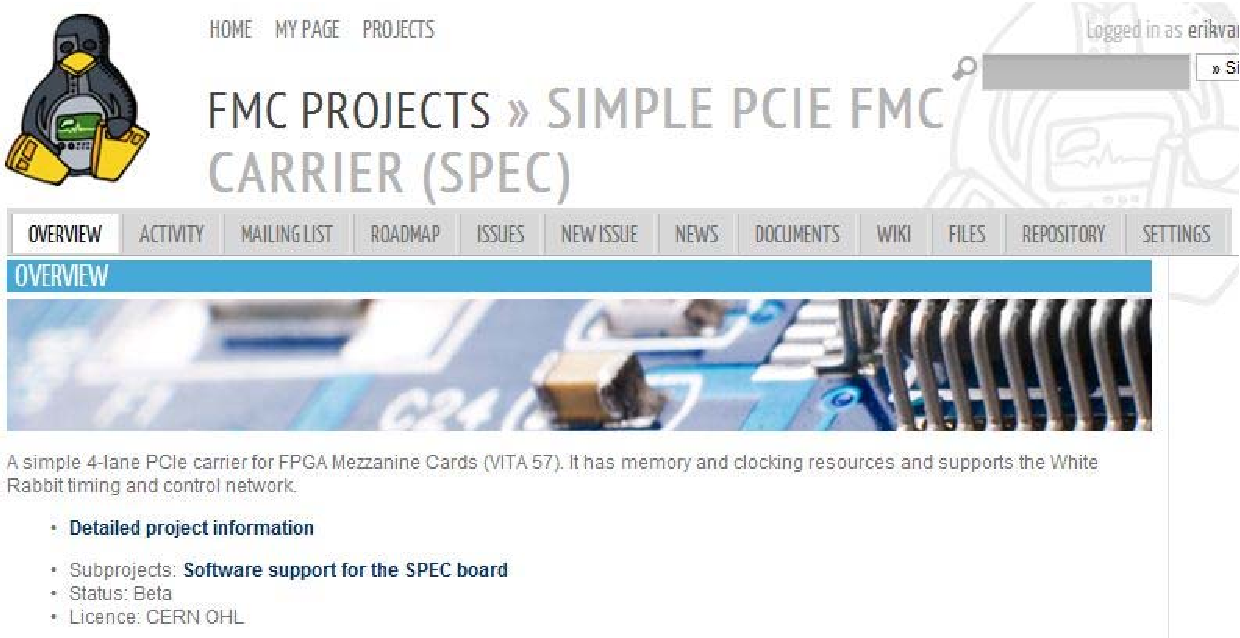
\includegraphics[height=6cm]{../../figures/ohwr/ohr_spec_top.eps}
 \end{center} 

\end{frame}
%%%%%%%%%%%%%%%%%%%%%%%%%%%%%%%%%%%%%%%%%%%%%%%%%%%%%%%%%%%%%%%%%%%%%%%%%%%%%%%%%%%%%%%%%%%%%%%%%%%%
%\section{Openness}
%\subsection{}
%%%%%%%%%%%%%%%%%%%%%%%%%%%%%%%%%%%%%%%%%%%%%%%%%%%%%%%%%%%%%%%%%%%%%%%%%%%%%%%%%%%%%%%%%%%%%%%%%%%%
\begin{frame}{CERN Open Hardware License \href{http://ohwr.org/cernohl}{-- ohwr.org/cernohl}}
    
    \begin{block}{Provides a solid legal basis}
      \begin{itemize}
        \item Open Software licences not usable (GNU, GPL, \dots)
        \item Developed by Knowledge and Technology Transfer Group
        \item Defines conditions of using \& modifying licenced material
      \end{itemize}
   \end{block}

   \begin{block}{Same principles as Open Software}
      \begin{itemize}
        \item Anyone can see the source (design documentation)
        \item Anyone is free to study, modify and share
        \item Any modification and distribution under same licence
        \item Persistence makes everyone profit from improvements
      \end{itemize}
   \end{block}

\end{frame}
%%%%%%%%%%%%%%%%%%%%%%%%%%%%%%%%%%%%%%%%%%%%%%%%%%%%%%%%%%%%%%%%%%%%%%%%%%%%%%%%%%%%%%%%%%%%%%%%%%%%
%\section{Applications}
%\subsection{Topology Redundancy}
%%%%%%%%%%%%%%%%%%%%%%%%%%%%%%%%%%%%%%%%%%%%%%%%%%%%%%%%%%%%%%%%%%%%%%%%%%%%%%%%%%%%%%%%%%%%%%%%%%%%
\begin{frame}{Example of mechanics licenced with the CERN OHL}
  \begin{center}
    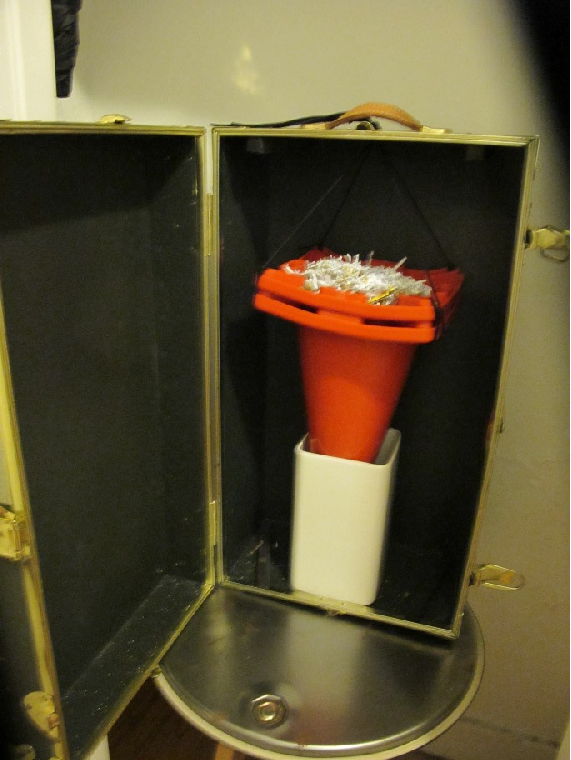
\includegraphics[height=5cm]{../../figures/ohwr/worm-farm-008.eps}
    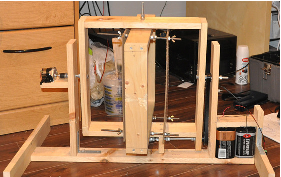
\includegraphics[height=5cm]{../../figures/ohwr/rotocaster.eps}
   Worm farm and rotocaster
 \end{center} 
\end{frame}
%%%%%%%%%%%%%%%%%%%%%%%%%%%%%%%%%%%%%%%%%%%%%%%%%%%%%%%%%%%%%%%%%%%%%%%%%%%%%%%%%%%%%%%%%%%%%%%%%%%%
%\section{Applications}
%\subsection{Topology Redundancy}
%%%%%%%%%%%%%%%%%%%%%%%%%%%%%%%%%%%%%%%%%%%%%%%%%%%%%%%%%%%%%%%%%%%%%%%%%%%%%%%%%%%%%%%%%%%%%%%%%%%%
\begin{frame}{Open Hardware - how does it work ?}

      \begin{center}
	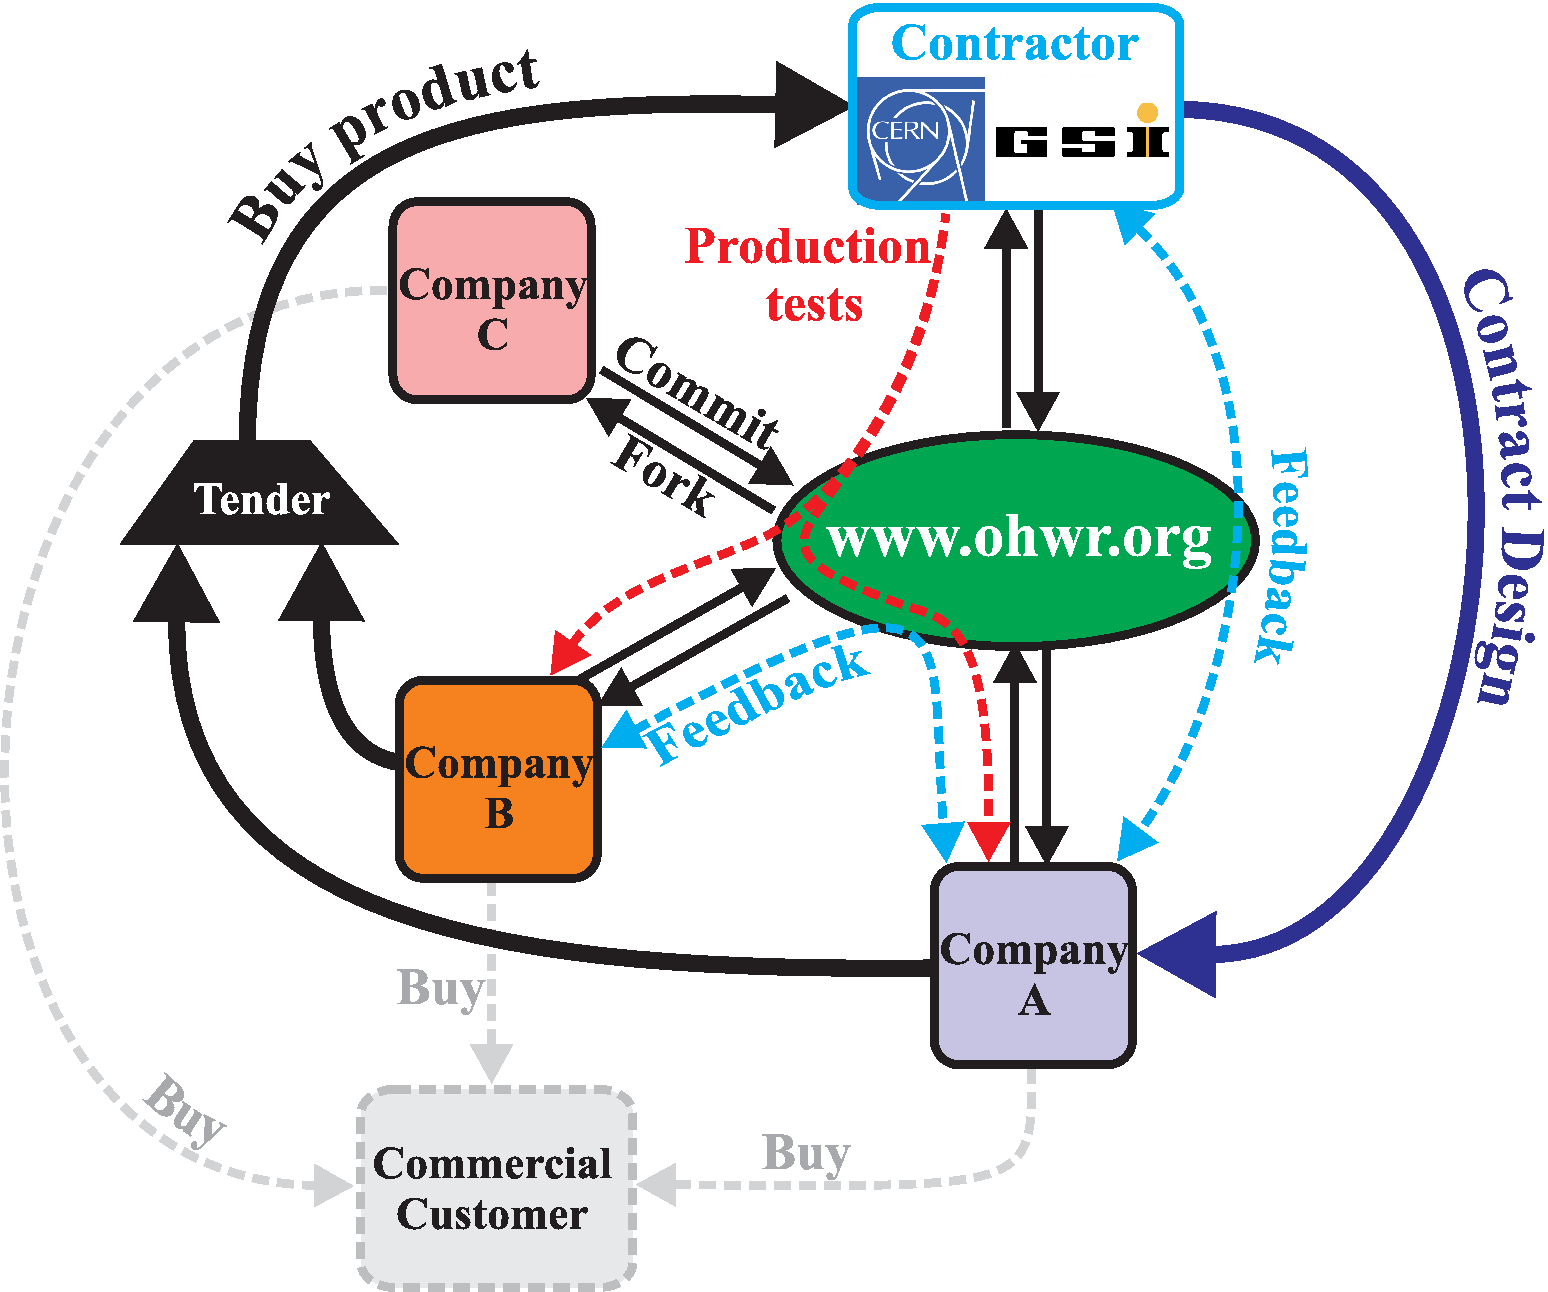
\includegraphics[height=0.8\textheight]{../../figures/ohwr/openHW.eps} 
      \end{center}

\end{frame}
%%%%%%%%%%%%%%%%%%%%%%%%%%%%%%%%%%%%%%%%%%%%%%%%%%%%%%%%%%%%%%%%%%%%%%%%%%%%%%%%%%%%%%%%%%%%%%%%%%%%
%\section{Applications}
%\subsection{Topology Redundancy}
%%%%%%%%%%%%%%%%%%%%%%%%%%%%%%%%%%%%%%%%%%%%%%%%%%%%%%%%%%%%%%%%%%%%%%%%%%%%%%%%%%%%%%%%%%%%%%%%%%%%
\begin{frame}{Open Hardware works}
	\begin{block}{Projects}
   \begin{itemize}
	\item 46 active projects
	\begin{itemize}
		\item 38 initiated by CERN groups, 8 by other institutes
	   \end{itemize}
	\item 3.6 developers on average 
   \end{itemize}
	\end{block}

\begin{block}{Types of designs}
\begin{itemize}
	\item About 30 hardware designs (of which 20 FMC projects)
	\item About 20 re-usable IP blocks
	\item General tools
	\begin{itemize}
		\item Production test environment (Python based)
		\item ADC performance test
%		\item Wishbone slave generator, crossbar
	\end{itemize}
   \end{itemize}
	\end{block}
\textcolor{gray}{data from October 2011}
\end{frame}
%%%%%%%%%%%%%%%%%%%%%%%%%%%%%%%%%%%%%%%%%%%%%%%%%%%%%%%%%%%%%%%%%%%%%%%%%%%%%%%%%%%%%%%%%%%%%%%%%%%%
\section{Summary}
\subsection{}
%%%%%%%%%%%%%%%%%%%%%%%%%%%%%%%%%%%%%%%%%%%%%%%%%%%%%%%%%%%%%%%%%%%%%%%%%%%%%%%%%%%%%%%%%%%%%%%%%%%%
\begin{frame}{Summary}


    \begin{itemize}
      \item Timing-wise WR is working now \textbf{focus on data}
      \item Interest of standardization bodies: WR presented to \textbf{ITU-T} and \textbf{IEEE}
      \item \textbf{First deployment} at CERN of WR timing and control network \textbf{for AD}
      \item Increasing number of applications
      \item First commercially available WR switch by the end of 2012

    \end{itemize}    

 
\end{frame}
%%%%%%%%%%%%%%%%%%%%%%%%%%%%%%%%%%%%%%%%%%%%%%%%%%%%%%%%%%%%%%%%%%%%%%%%%%%%%%%%%%%%%%%%%%%%%%%%%%%%
%\section{Applications}
%\subsection{Topology Redundancy}
%%%%%%%%%%%%%%%%%%%%%%%%%%%%%%%%%%%%%%%%%%%%%%%%%%%%%%%%%%%%%%%%%%%%%%%%%%%%%%%%%%%%%%%%%%%%%%%%%%%%
\begin{frame}{White Rabbits Family}
\begin{columns}[c]
\column{2.0in}
    \begin{center}
    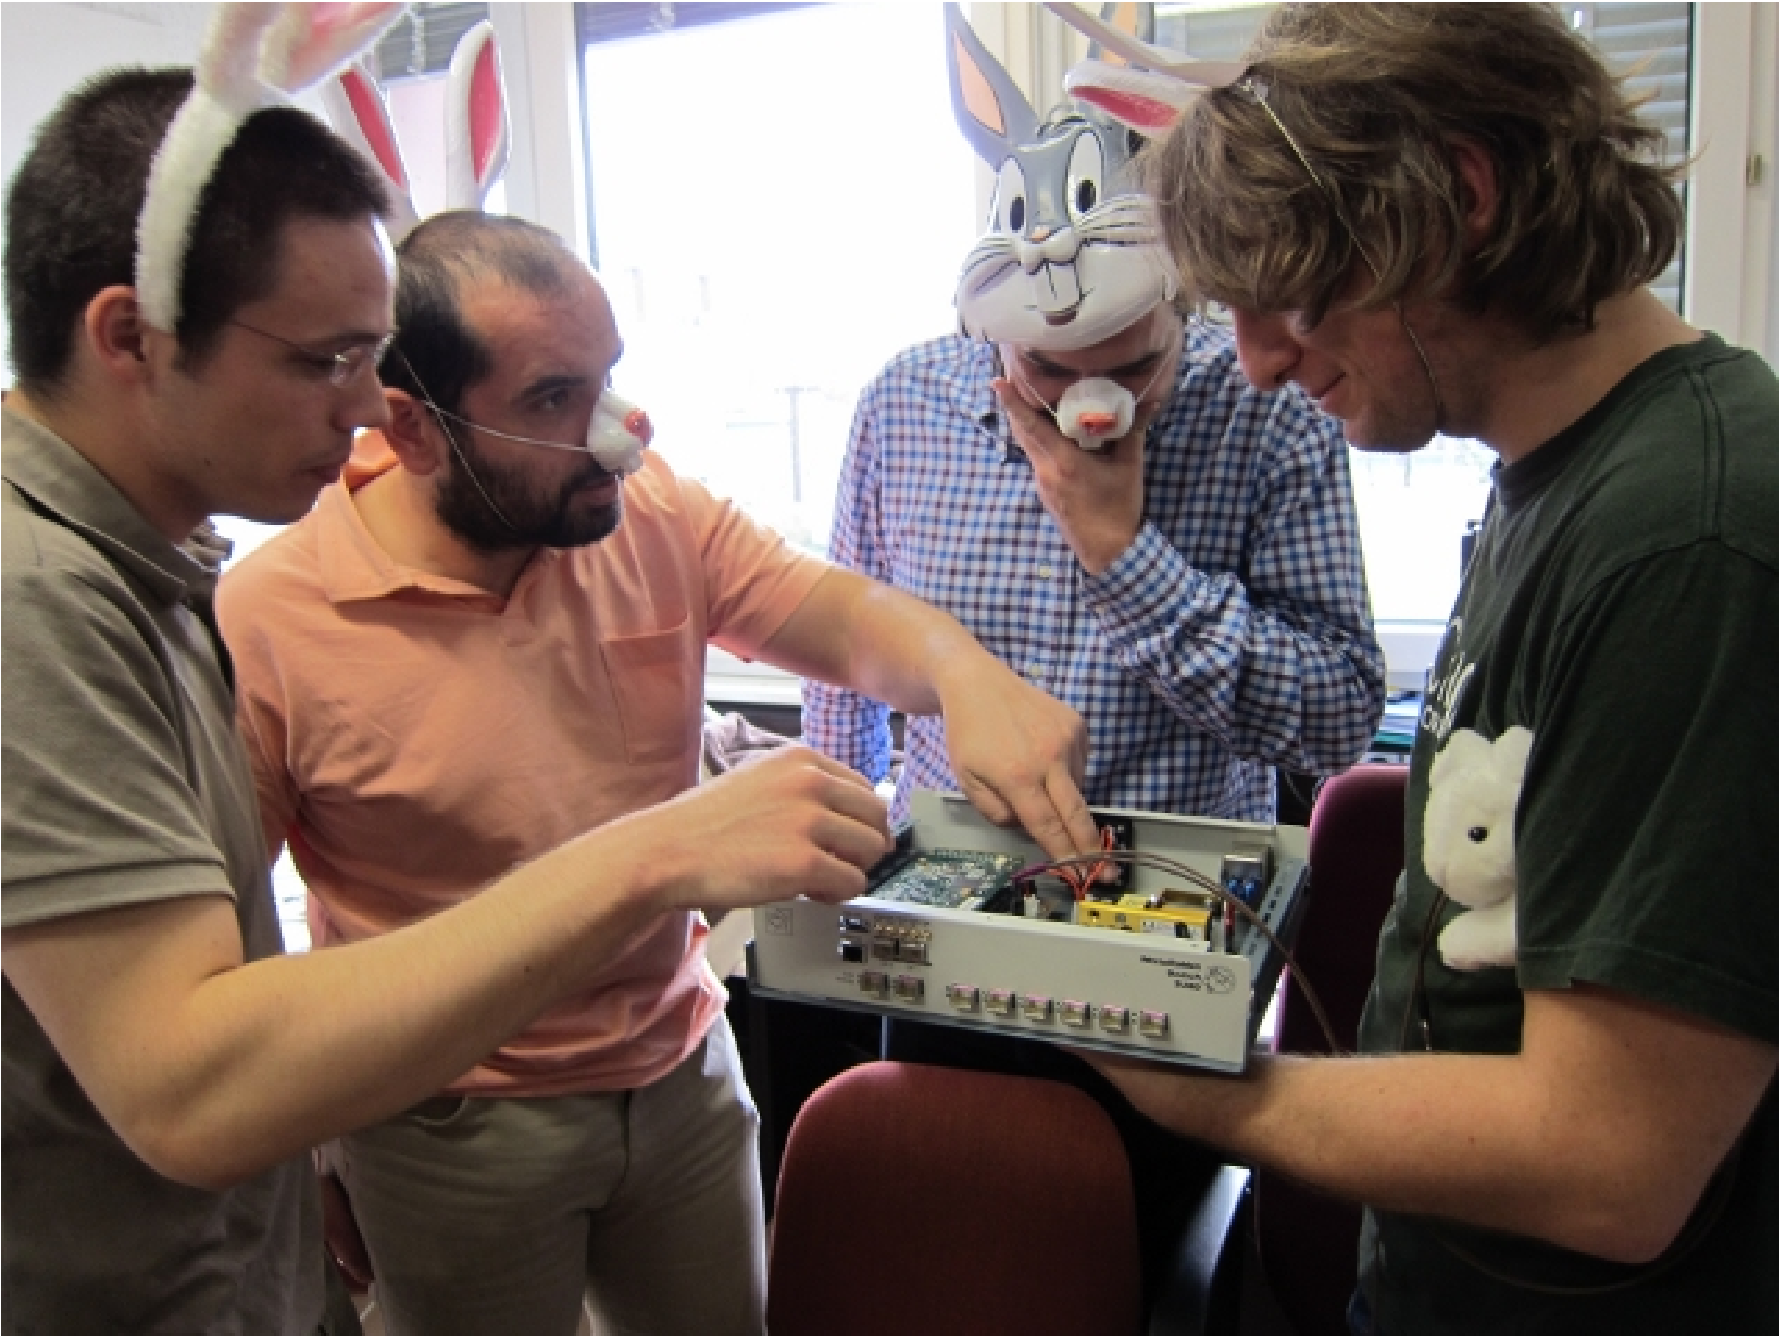
\includegraphics[width=3.5cm]{../../figures/misc/fourRabbits.ps}
    \end{center}
\column{2.0in}
    \begin{center}
    $\Leftarrow$ CERN geeks :) \\
    All the family \\
    $\Downarrow$
     \end{center}
\end{columns}

\begin{center}
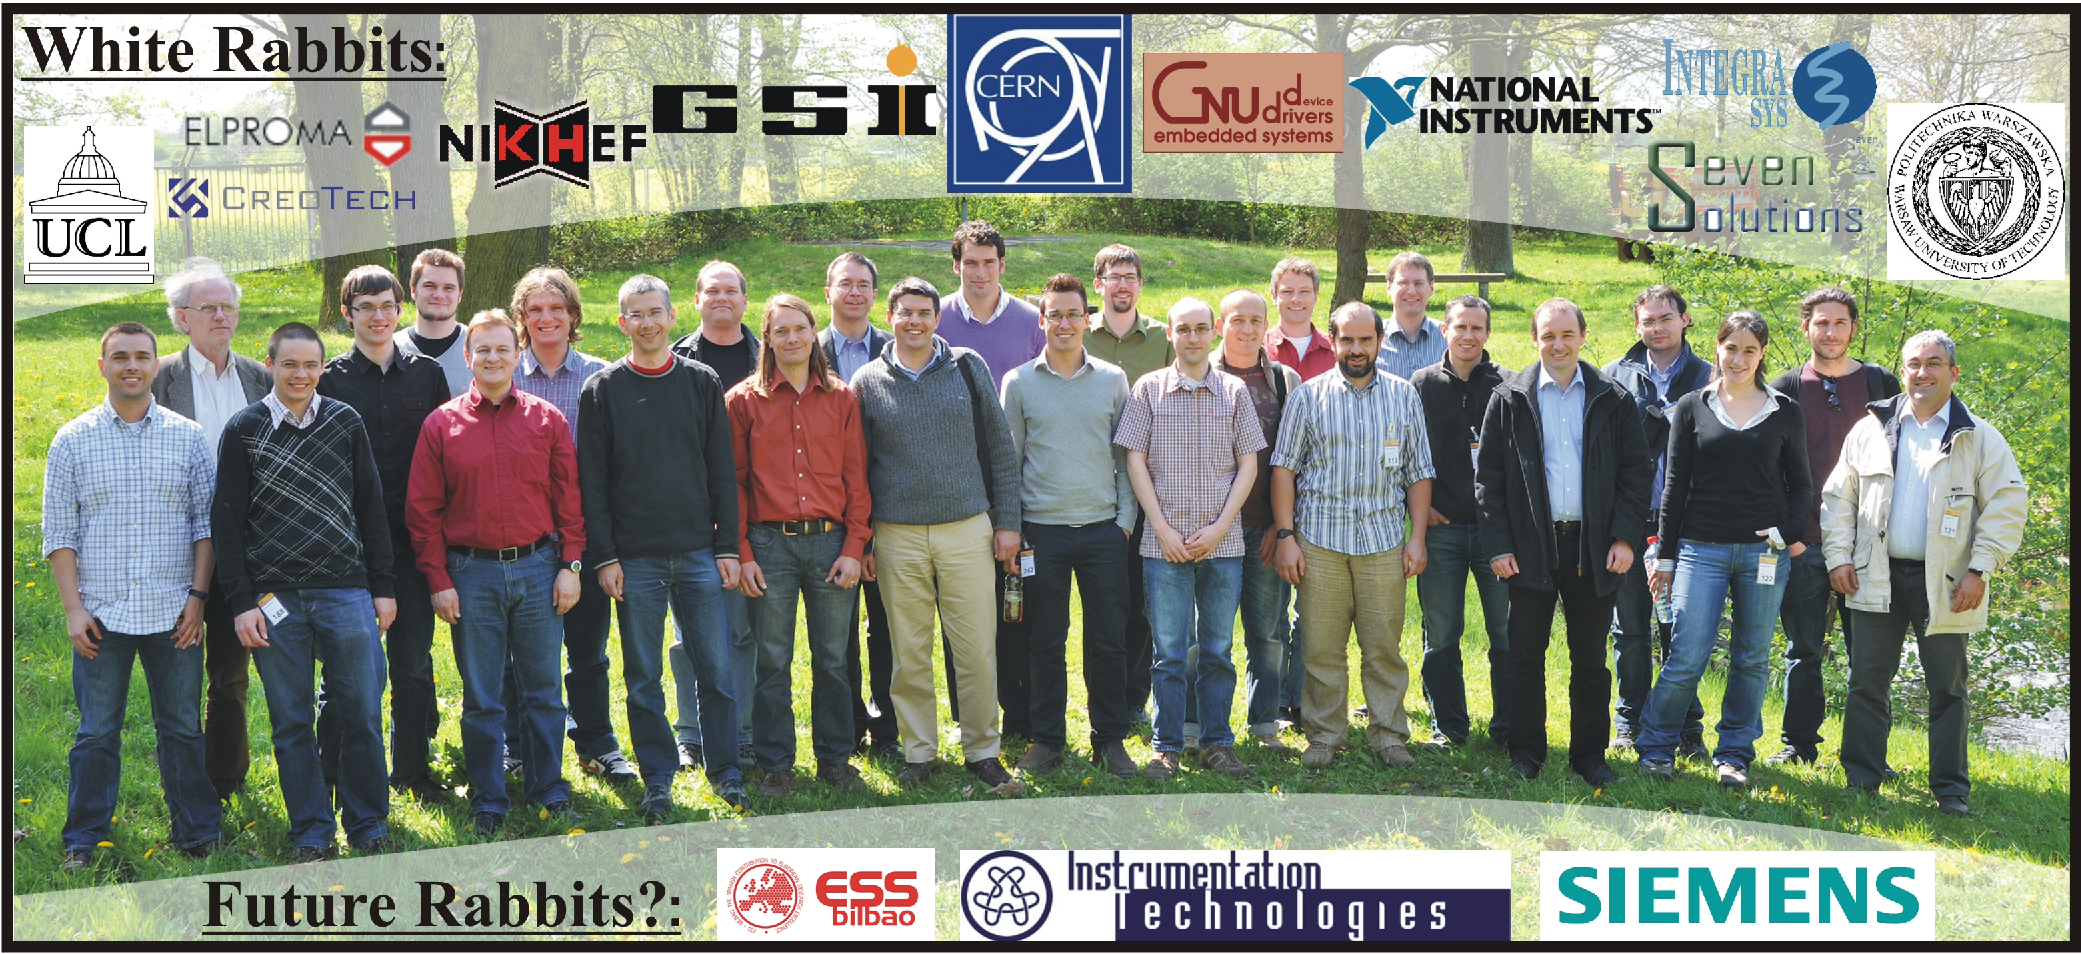
\includegraphics[width=9.5cm]{../../figures/misc/WRfamily.ps}
\end{center}
\end{frame}
%%%%%%%%%%%%%%%%%%%%%%%%%%%%%%%%%%%%%%%%%%%%%%%%%%%%%%%%%%%%%%%%%%%%%%%%%%%%%%%%%%%%%%%%%%%%%%%%%%%%
\section{Q\&A}
\subsection{}
%%%%%%%%%%%%%%%%%%%%%%%%%%%%%%%%%%%%%%%%%%%%%%%%%%%%%%%%%%%%%%%%%%%%%%%%%%%%%%%%%%%%%%%%%%%%%%%%%%%%
\begin{frame}{Questions and answers}

    \begin{center}
    \includegraphics[height=4.0cm]{../../figures/logo/WRlogo.ps}
    \end{center}

\end{frame}

\appendix
\backupbegin

%%%%%%%%%%%%%%%%%%%%%%%%%%%%%%%%%%%%%%%%%%%%%%%%%%%%%%%%%%%%%%%%%%%%%%%%%%%%%%%%%%%%%%%%%%%%%%%%%%%%
%\section{extras}
% \subsection{}
%%%%%%%%%%%%%%%%%%%%%%%%%%%%%%%%%%%%%%%%%%%%%%%%%%%%%%%%%%%%%%%%%%%%%%%%%%%%%%%%%%%%%%%%%%%%%%%%%%%%
\begin{frame}{Extras}

    \begin{center}
      Extras
    \end{center}

\end{frame}

%%%%%%%%%%%%%%%%%%%%%%%%%%%%%%%%%%%%%%%%%%%%%%%%%%%%%%%%%%%%%%%%%%%%%%%%%%%%%%%%%%%%%%%%%%%%%%%%%%%%
\section{CERN control system}
\subsection{}
%%%%%%%%%%%%%%%%%%%%%%%%%%%%%%%%%%%%%%%%%%%%%%%%%%%%%%%%%%%%%%%%%%%%%%%%%%%%%%%%%%%%%%%%%%%%%%%%%%%%
\begin{frame}{CERN}

\begin{columns}[c]
  \column{0.55\textwidth}
    \begin{center}

      \begin{itemize}
	\item 6 accelerators
	\item LHC: 27km perimeter
	\item Thousands of devices to be controlled and synchronized
	\item A huge real-time distributed system
      \end{itemize}

    \end{center}
  \column{0.6\textwidth}
    \begin{center}
      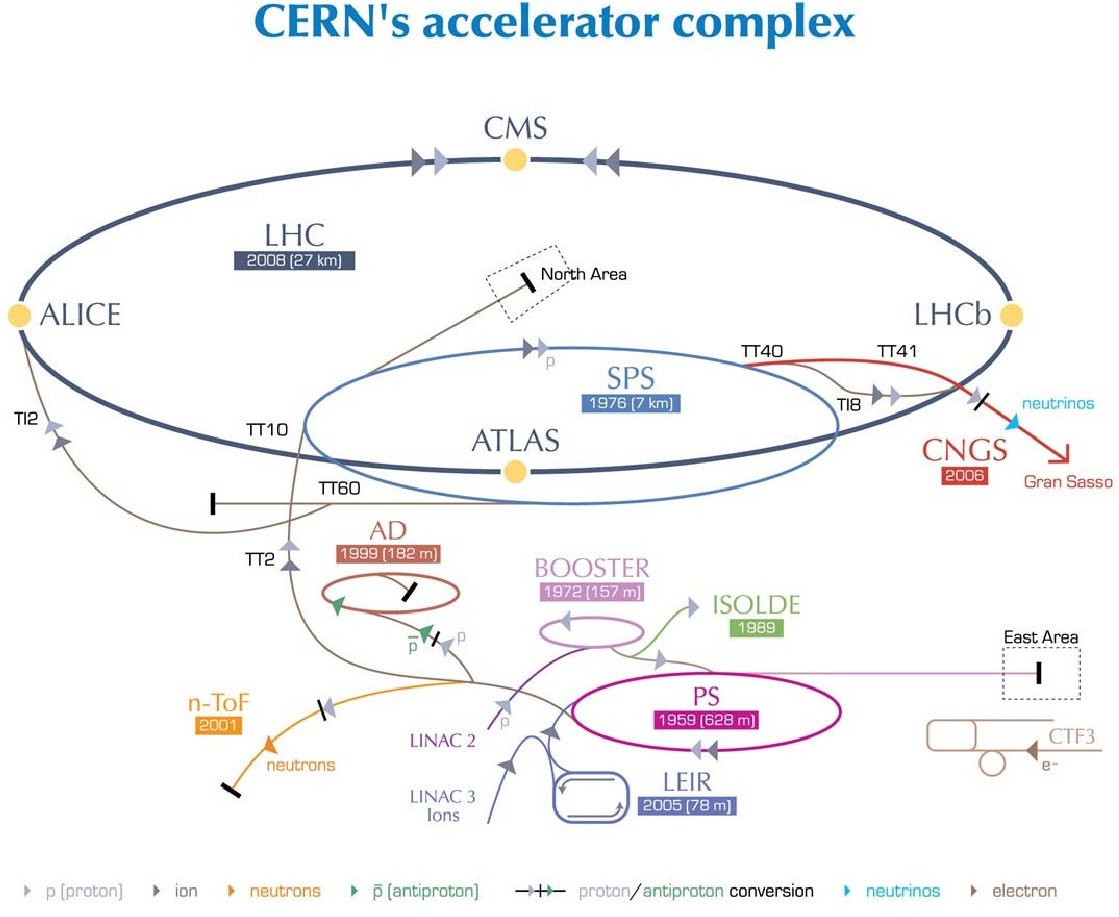
\includegraphics[width=6.5cm]{../../figures/applications/CERN/accelerators.eps}
    \end{center}
\end{columns}

\end{frame}
%%%%%%%%%%%%%%%%%%%%%%%%%%%%%%%%%%%%%%%%%%%%%%%%%%%%%%%%%%%%%%%%%%%%%%%%%%%%%%%%%%%%%%%%%%%%%%%%%%%%
% \section{}
% \subsection{}
%%%%%%%%%%%%%%%%%%%%%%%%%%%%%%%%%%%%%%%%%%%%%%%%%%%%%%%%%%%%%%%%%%%%%%%%%%%%%%%%%%%%%%%%%%%%%%%%%%%%
\begin{frame}{A simplified explanation of CERN control system (1)}

      \begin{center}
      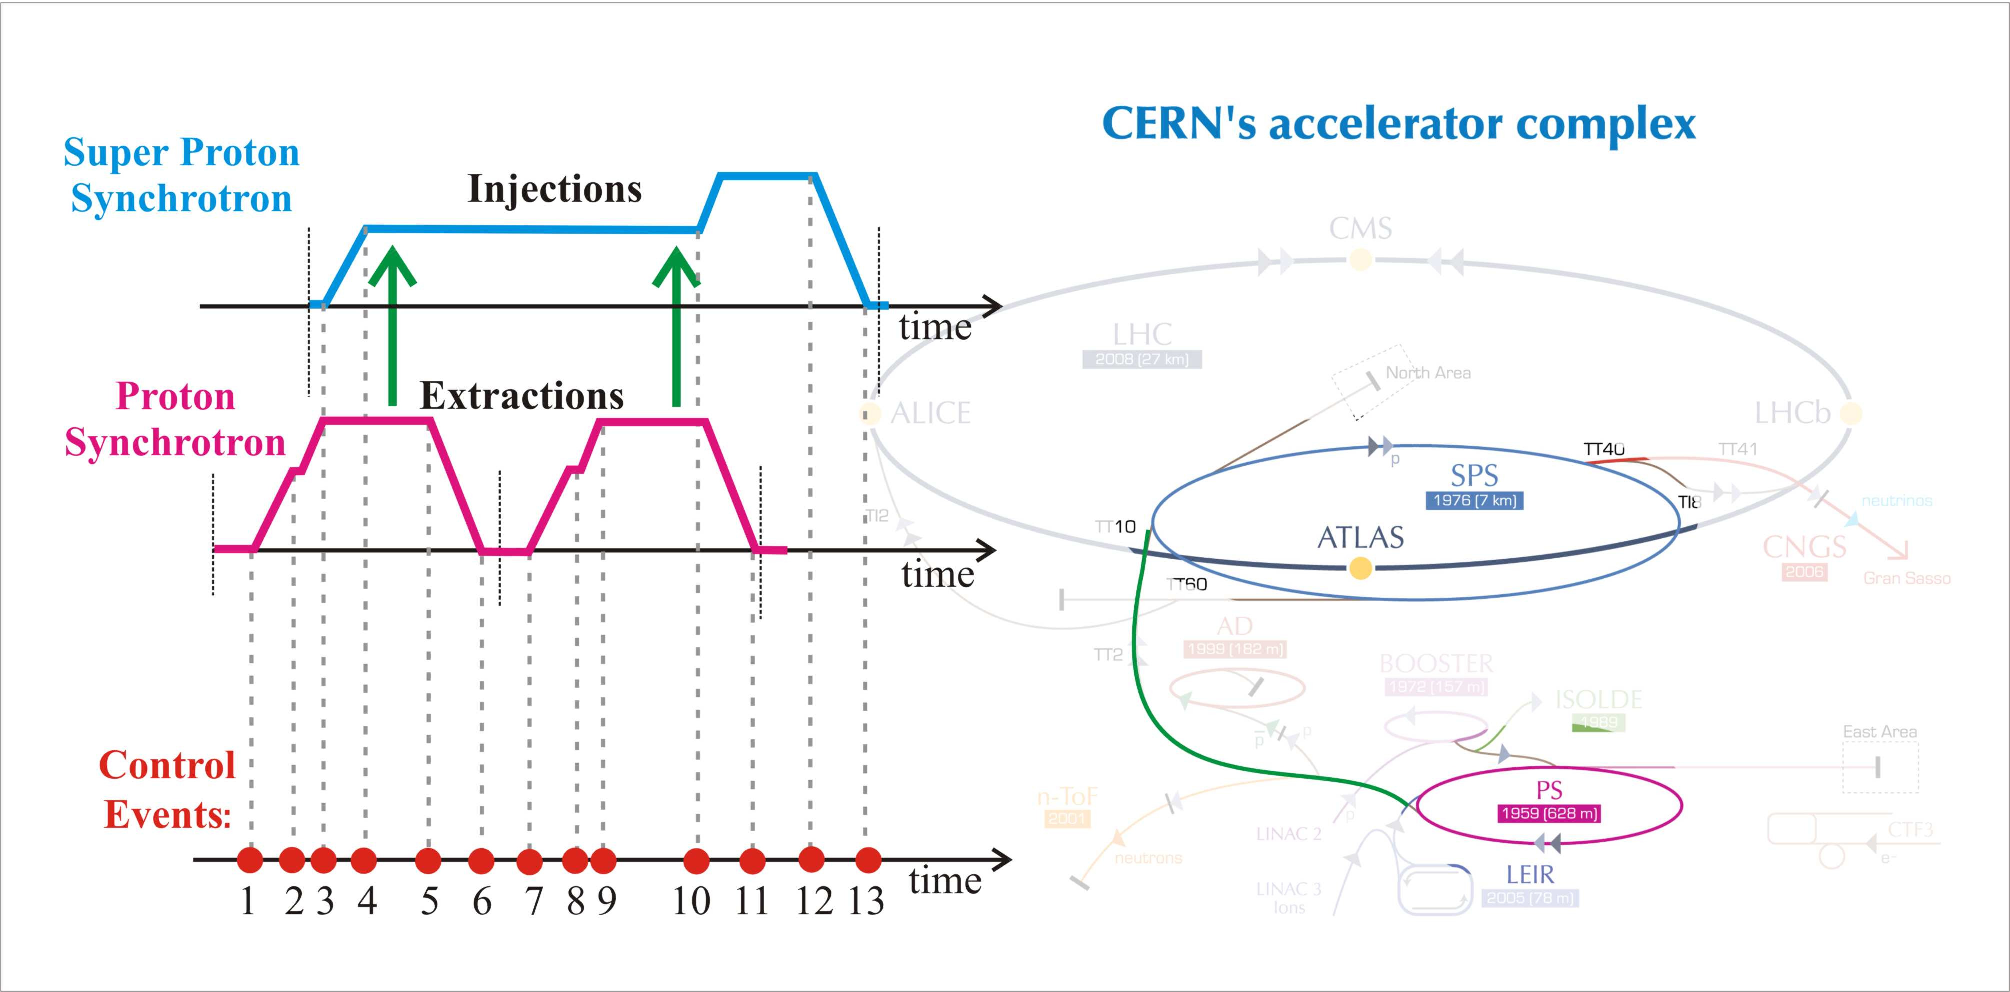
\includegraphics[width=1.0\textwidth]{../../figures/applications/CERN/event1.eps}
      \end{center}

  \begin{itemize}
    \item {\bf Events} -- points in time at which actions are triggered
    \item Each event is identified by an {\bf ID}
  \end{itemize}

\end{frame}


%%%%%%%%%%%%%%%%%%%%%%%%%%%%%%%%%%%%%%%%%%%%%%%%%%%%%%%%%%%%%%%%%%%%%%%%%%%%%%%%%%%%%%%%%%%%%%%%%%%%
% \section{}
% \subsection{}
%%%%%%%%%%%%%%%%%%%%%%%%%%%%%%%%%%%%%%%%%%%%%%%%%%%%%%%%%%%%%%%%%%%%%%%%%%%%%%%%%%%%%%%%%%%%%%%%%%%%
\begin{frame}{A simplified explanation of CERN control system (2)}

      \begin{center}
      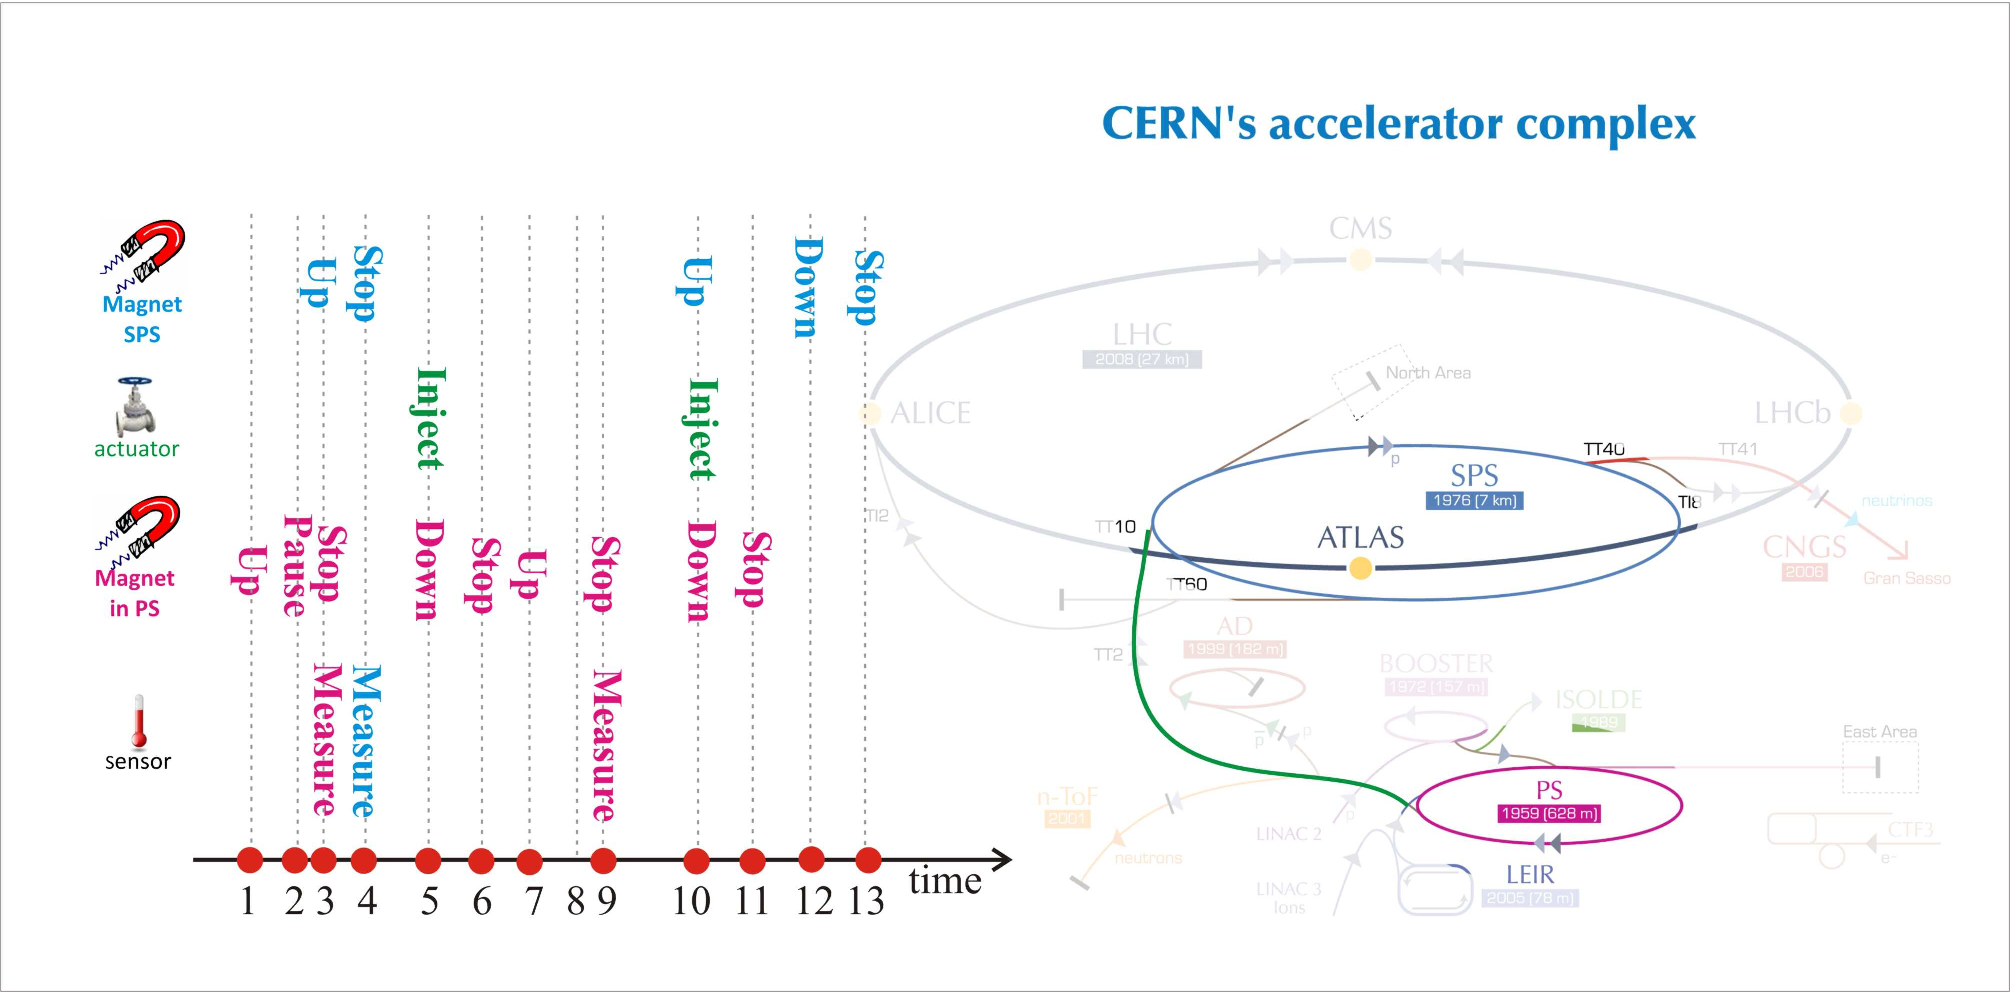
\includegraphics[width=1.0\textwidth]{../../figures/applications/CERN/event2.eps}
      \end{center}

  \begin{itemize}
    \item Devices are subscribed to events 
    \item Each device "knows" what to do on particular event
  \end{itemize}


\end{frame}


%%%%%%%%%%%%%%%%%%%%%%%%%%%%%%%%%%%%%%%%%%%%%%%%%%%%%%%%%%%%%%%%%%%%%%%%%%%%%%%%%%%%%%%%%%%%%%%%%%%%
% \section{}
% \subsection{}
%%%%%%%%%%%%%%%%%%%%%%%%%%%%%%%%%%%%%%%%%%%%%%%%%%%%%%%%%%%%%%%%%%%%%%%%%%%%%%%%%%%%%%%%%%%%%%%%%%%%
\begin{frame}{A simplified explanation of CERN control system (3)}

      \begin{center}
      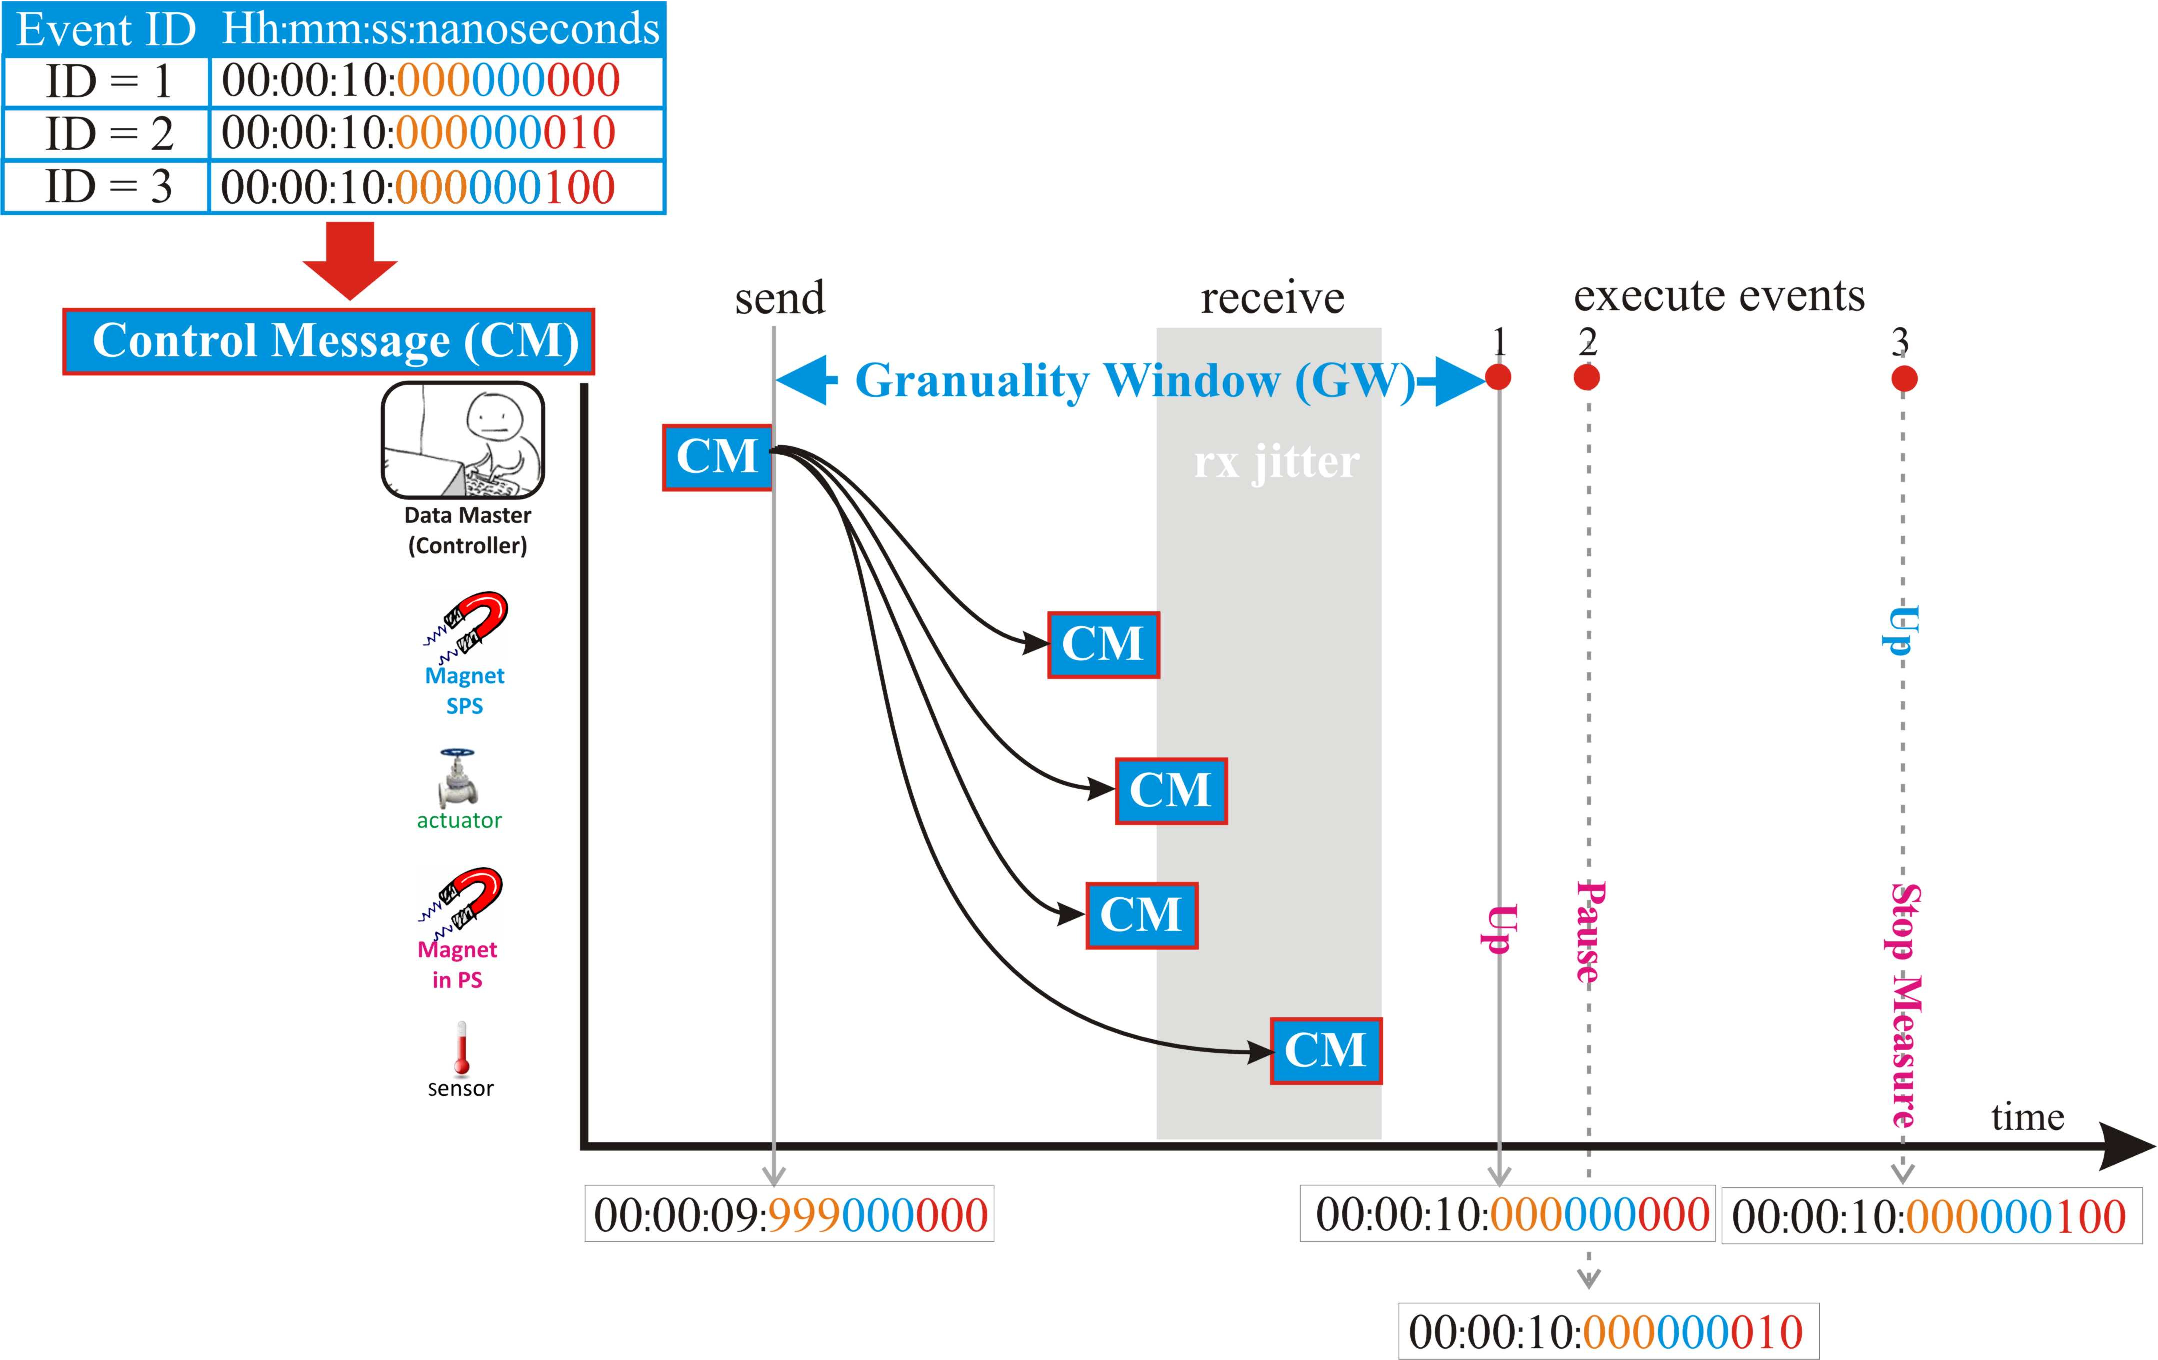
\includegraphics[width=.8\textwidth]{../../figures/applications/CERN/event3.eps}
      \end{center}

  \begin{itemize}
    \item Each event (ID) has a trigger time associated
	\item A set of events is sent as a single {\bf Control Message (CM)}
	\item CM is broadcast to all the end devices (nodes)
	\item CM is sent in advance ({\bf Granularity Window})
  \end{itemize}

\end{frame}

%%%%%%%%%%%%%%%%%%%%%%%%%%%%%%%%%%%%%%%%%%%%%%%%%%%%%%%%%%%%%%%%%%%%%%%%%%%%%%%%%%%%%%%%%%%%%%%%%%%%
% \section{}
% \subsection{}
%%%%%%%%%%%%%%%%%%%%%%%%%%%%%%%%%%%%%%%%%%%%%%%%%%%%%%%%%%%%%%%%%%%%%%%%%%%%%%%%%%%%%%%%%%%%%%%%%%%%
\begin{frame}{A simplified explanation of CERN control system (4)}

\begin{columns}[c]
  \column{0.55\textwidth}
   {\bf Granuality Window: }
    \begin{center}
      \begin{itemize}
	    \item Controller-input to node-output (i.e. pulse)
	    \item Maximum bound latency {\bf guaranteed } by the system
	    \item Processing and network latency included
      \end{itemize}

    \end{center}
  \column{0.6\textwidth}
    \begin{center}
      \begin{center}
      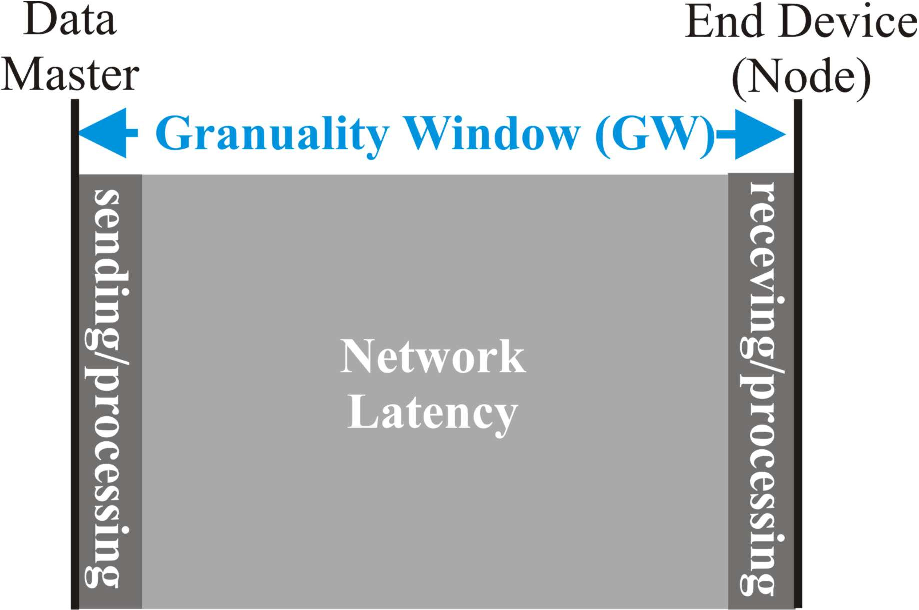
\includegraphics[width=.8\textwidth]{../../figures/applications/CERN/gw.eps}
      \end{center}
    \end{center}
\end{columns}

\end{frame}

%%%%%%%%%%%%%%%%%%%%%%%%%%%%%%%%%%%%%%%%%%%%%%%%%%%%%%%%%%%%%%%%%%%%%%%%%%%%%%%%%%%%%%%%%%%%%%%%%%%%
% \section{}
% \subsection{}
%%%%%%%%%%%%%%%%%%%%%%%%%%%%%%%%%%%%%%%%%%%%%%%%%%%%%%%%%%%%%%%%%%%%%%%%%%%%%%%%%%%%%%%%%%%%%%%%%%%%
\begin{frame}{A simplified explanation of CERN control system (5)}

      \begin{center}
      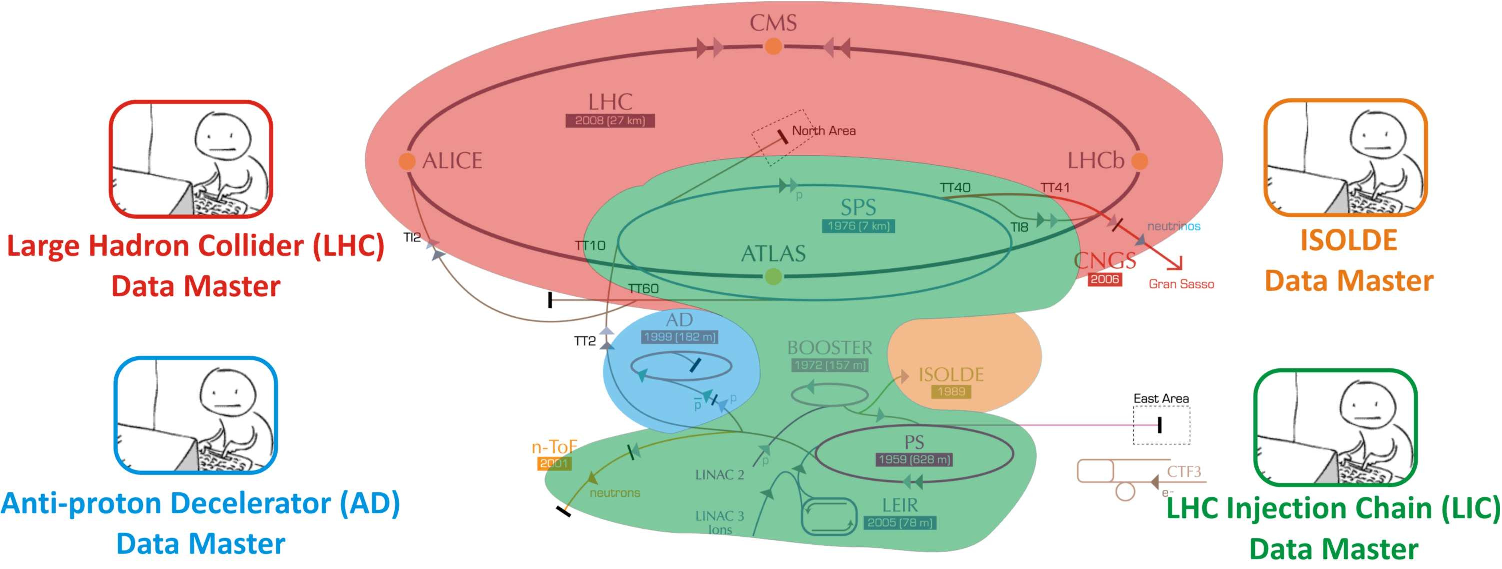
\includegraphics[width=.7\textwidth]{../../figures/applications/CERN/accNetworks.eps}
      \end{center}

  \begin{itemize}
    \item 4 accelerator networks
    \item Separate {\bf Data Master (DM)} for each network
    \item \textcolor{green!90}{LIC Data Master} communicates with other DMs and control devices in their networks
    \item Broadcast of {\bf Control Messages} within network(s)
  \end{itemize}

\end{frame}

%%%%%%%%%%%%%%%%%%%%%%%%%%%%%%%%%%%%%%%%%%%%%%%%%%%%%%%%%%%%%%%%%%%%%%%%%%%%%%%%%%%%%%%%%%%%%%%%%%%%
% \subsection{}
%%%%%%%%%%%%%%%%%%%%%%%%%%%%%%%%%%%%%%%%%%%%%%%%%%%%%%%%%%%%%%%%%%%%%%%%%%%%%%%%%%%%%%%%%%%%%%%%%%%%
\begin{frame}{Time Distribution in White Rabbit}

  \begin{itemize}
    \item Synchronization with {\bf sub-ns} accuracy over fiber
    \item Combination of
	\begin{itemize}
	  \item Precision Time Protocol ({\bf PTP}) synchronization
	  \item Synchronous Ethernet ({\bf SyncE}) syntonization
	  \item Digital Dual-Mixer Time Difference ({\bf DDMTD}) phase detection
	\end{itemize}
%    \item Reliability-oriented.
    \item WR Link:
  \end{itemize}

  \begin{center}
  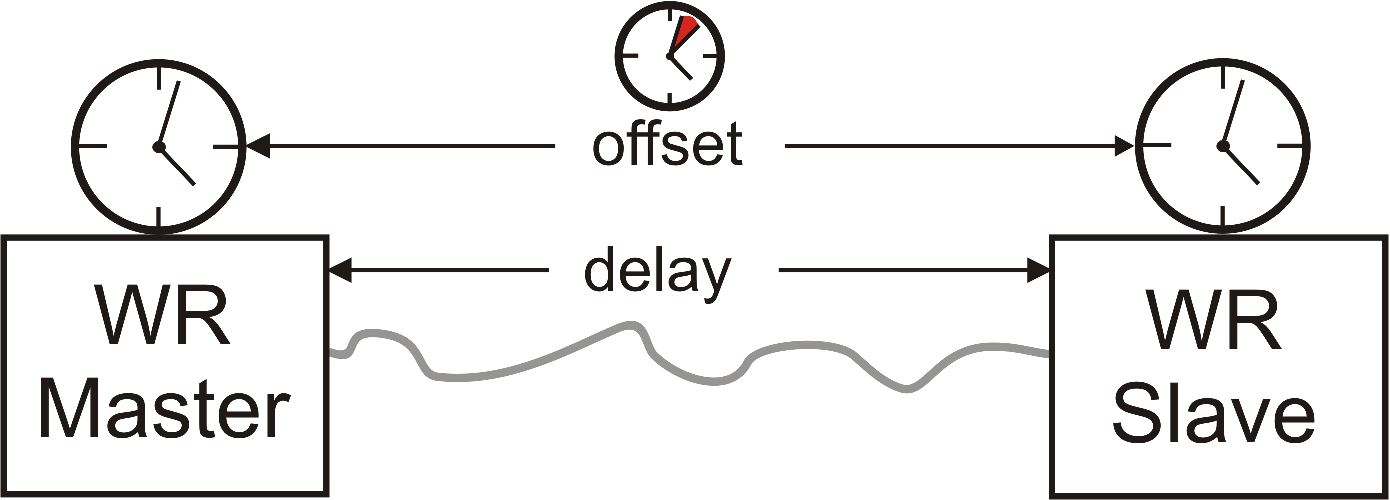
\includegraphics[height=3cm]{../../figures/protocol/wrLink.ps}
  \end{center}

\end{frame}
%%%%%%%%%%%%%%%%%%%%%%%%%%%%%%%%%%%%%%%%%%%%%%%%%%%%%%%%%%%%%%%%%%%%%%%%%%%%%%%%%%%%%%%%%%%%%%%%%%%%
\section{White Rabbit PTP}
\subsection{}
% %%%%%%%%%%%%%%%%%%%%%%%%%%%%%%%%%%%%%%%%%%%%%%%%%%%%%%%%%%%%%%%%%%%%%%%%%%%%%%%%%%%%%%%%%%%%%%%%%%%%
\begin{frame}{PTP is OK but ...}

  \resizebox{11cm}{!} 
  {
    \begin{tabular}{ r c l }
  {\bf What are the issues...} 	& {\bf and}      & {\bf ... how we address them}  \\
				&     		 &        \\
      PTP-base		 	& \multirow{2}{*}{$\Rightarrow$}  & \multirow{2}{*}{SyncE }\\
      syntonization	        &      		 &        \\
				&      		 &        			\\
      limited             	&\multirow{2}{*}{$\Rightarrow$}  	 & SyncE \\
      precision and resolution  &      		 & DDTMD phase detection\\
				&    		 &        \\
			        &      		 & SyncE  \\
      unknown link asymmetry    & $\Rightarrow$  & DDTMD phase detection \\
				&      		 & WR Link Delay Model \\
				&      		 &        \\
      \multicolumn{3}{c}{WR extension to PTP ({\bf WRPTP}) for } \\
      \multicolumn{3}{c}{extra data exchange and logic} \\
    \end{tabular}
  }
\end{frame}
%%%%%%%%%%%%%%%%%%%%%%%%%%%%%%%%%%%%%%%%%%%%%%%%%%%%%%%%%%%%%%%%%%%%%%%%%%%%%%%%%%%%%%%%%%%%%%%%%%%%
%\section{Timestamps}
\subsection{}
%%%%%%%%%%%%%%%%%%%%%%%%%%%%%%%%%%%%%%%%%%%%%%%%%%%%%%%%%%%%%%%%%%%%%%%%%%%%%%%%%%%%%%%%%%%%%%%%%%%%
\begin{frame}{Fine Delay Measurement}

  \begin{center}
  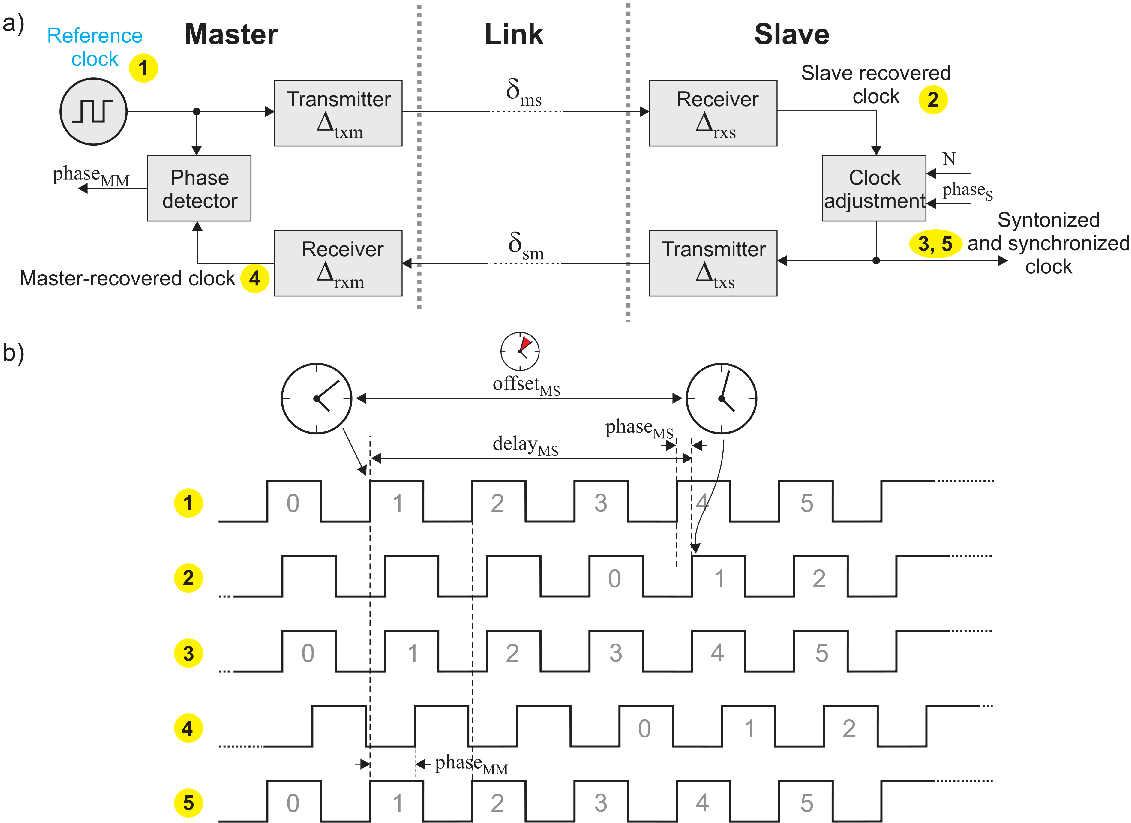
\includegraphics[width=10.0cm]{../../figures/protocol/link_model.eps}
  \end{center}

\end{frame}
%%%%%%%%%%%%%%%%%%%%%%%%%%%%%%%%%%%%%%%%%%%%%%%%%%%%%%%%%%%%%%%%%%%%%%%%%%%%%%%%%%%%%%%%%%%%%%%%%%%%
%\section{Link Asymmetry}
% \subsection{}
%%%%%%%%%%%%%%%%%%%%%%%%%%%%%%%%%%%%%%%%%%%%%%%%%%%%%%%%%%%%%%%%%%%%%%%%%%%%%%%%%%%%%%%%%%%%%%%%%%%%
\begin{frame}{Link Asymmetry}

  \begin{center}
  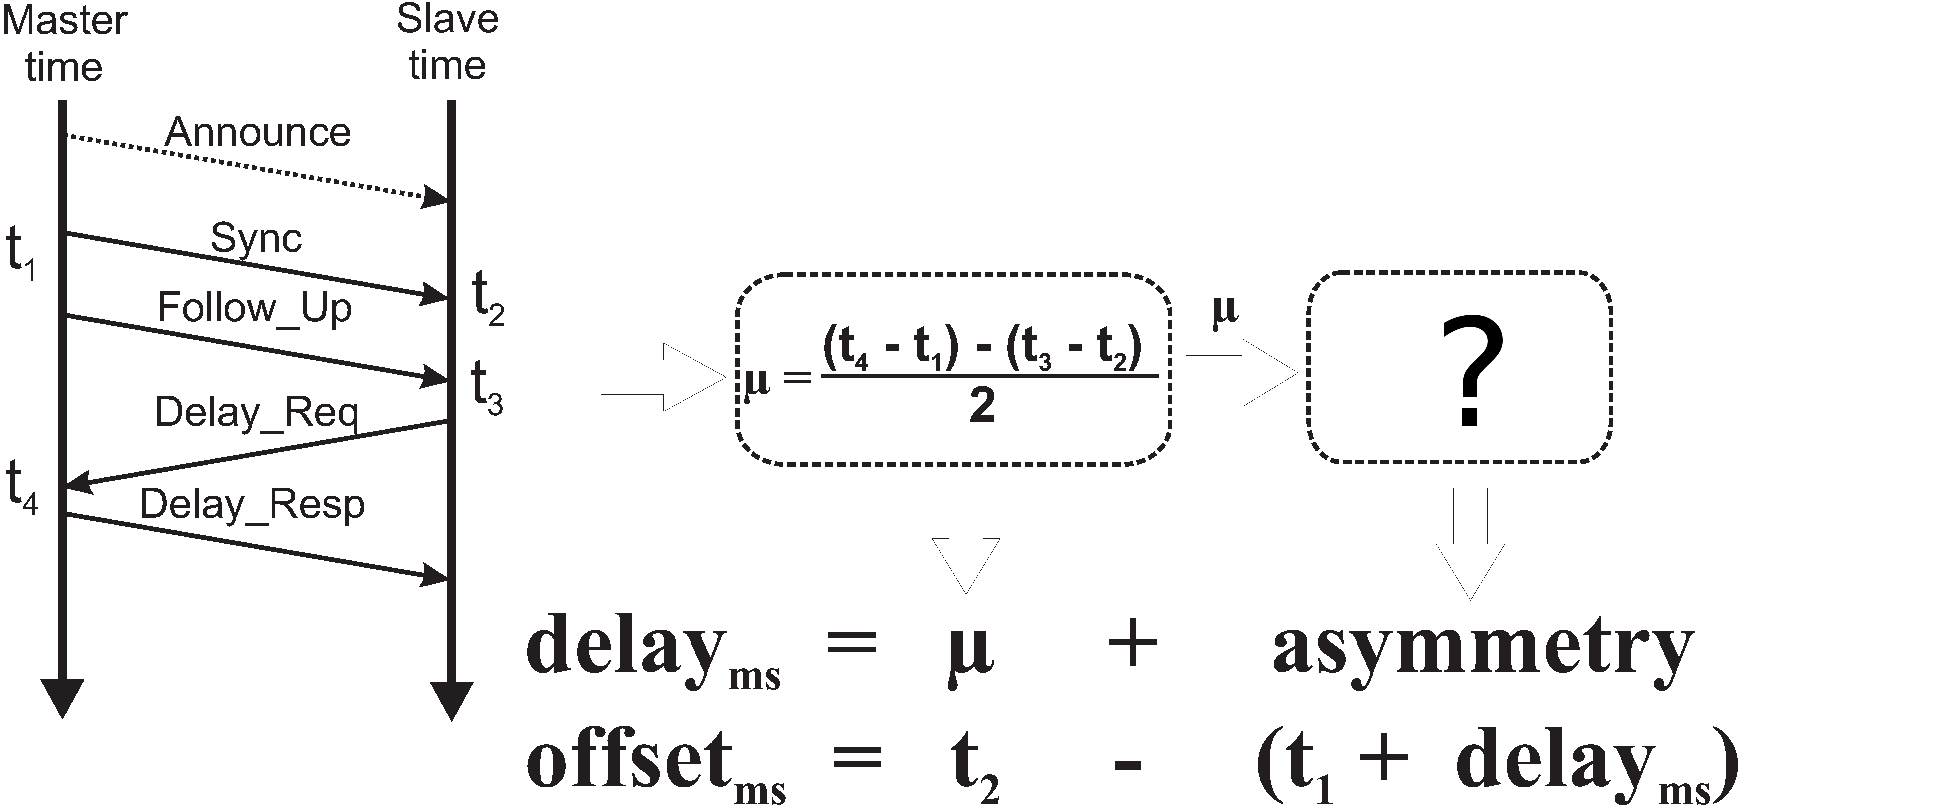
\includegraphics[height=4cm]{../../figures/protocol/wrLinkModel_init.eps}
  \end{center}

\end{frame}

%%%%%%%%%%%%%%%%%%%%%%%%%%%%%%%%%%%%%%%%%%%%%%%%%%%%%%%%%%%%%%%%%%%%%%%%%%%%%%%%%%%%%%%%%%%%%%%%%%%%
%\section{Link Delay Model}
%\subsection{}
%%%%%%%%%%%%%%%%%%%%%%%%%%%%%%%%%%%%%%%%%%%%%%%%%%%%%%%%%%%%%%%%%%%%%%%%%%%%%%%%%%%%%%%%%%%%%%%%%%%%
\begin{frame}{Link Delay Model}

  \begin{align}
    \nonumber delay_{ms} &= \Delta_{tx_m} + \delta_{ms} + \Delta_{rx_s} \\
    \nonumber delay_{sm} &= \Delta_{tx_s} + \delta_{sm} + \Delta_{rx_m}
  \end{align}

   \vspace{0.2cm}

  \begin{center}
  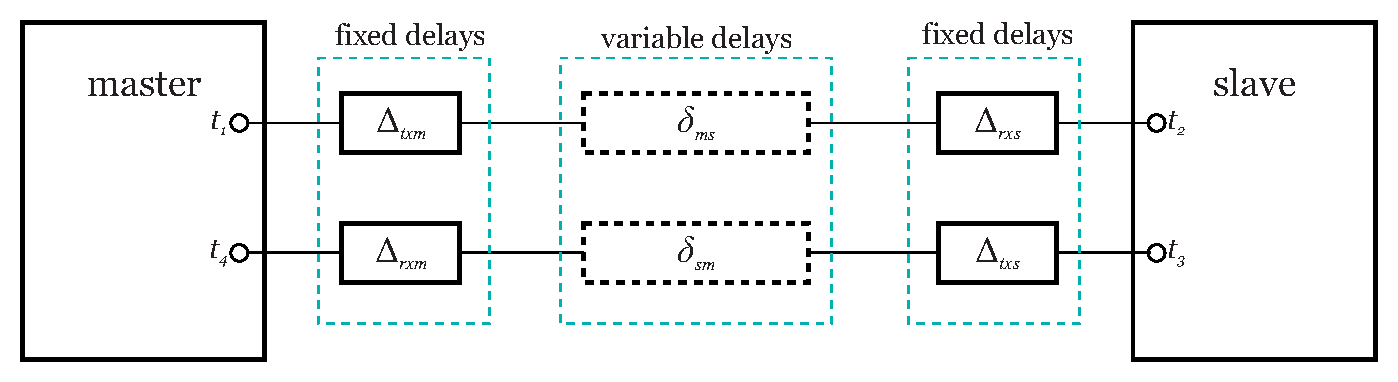
\includegraphics[height=2.5cm]{../../figures/protocol/delaymodel.eps}
  \end{center}

\begin{columns}[c]
  \column{2.8in}

    \begin{center}
      \textbf{Relative Delay Coefficient ($\alpha$)} \\
      for 1000BASE-BX10 over a Single-mode Optical Fiber
    \end{center}

  \column{1.5in}
    \begin{center}
      \begin{equation}
      \nonumber \delta_{ms} = (1 + \alpha) \, \delta_{sm}
      \end{equation}
    \end{center}
    \vspace{0.5cm}
\end{columns}
  
\end{frame}
%%%%%%%%%%%%%%%%%%%%%%%%%%%%%%%%%%%%%%%%%%%%%%%%%%%%%%%%%%%%%%%%%%%%%%%%%%%%%%%%%%%%%%%%%%%%%%%%%%%%
%\section{Link Delay Model}
% \subsection{}
%%%%%%%%%%%%%%%%%%%%%%%%%%%%%%%%%%%%%%%%%%%%%%%%%%%%%%%%%%%%%%%%%%%%%%%%%%%%%%%%%%%%%%%%%%%%%%%%%%%%
\begin{frame}{Fixed Delays}

  \begin{center}
  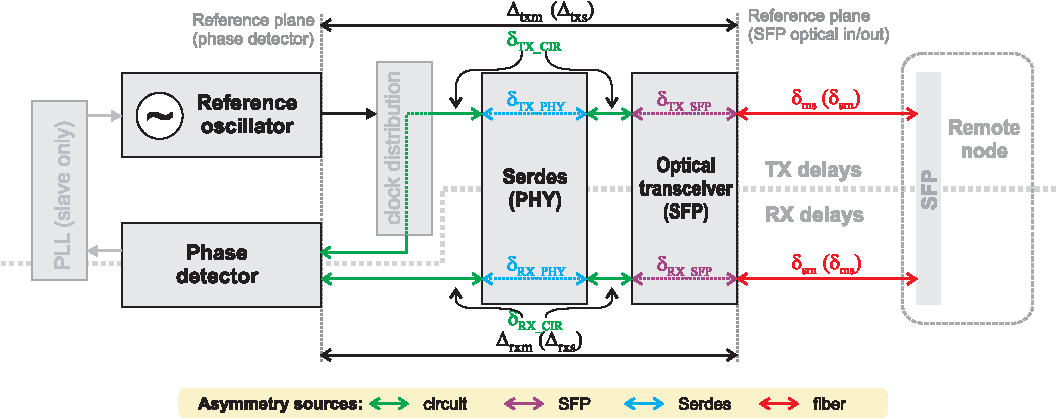
\includegraphics[width=11.0cm]{../../figures/protocol/asymmetries.eps}
  \end{center}

\end{frame}

%%%%%%%%%%%%%%%%%%%%%%%%%%%%%%%%%%%%%%%%%%%%%%%%%%%%%%%%%%%%%%%%%%%%%%%%%%%%%%%%%%%%%%%%%%%%%%%%%%%%
% \subsection{}
%%%%%%%%%%%%%%%%%%%%%%%%%%%%%%%%%%%%%%%%%%%%%%%%%%%%%%%%%%%%%%%%%%%%%%%%%%%%%%%%%%%%%%%%%%%%%%%%%%%%
\begin{frame}{Link Delay Model: fiber optic solution}

  \begin{center}
  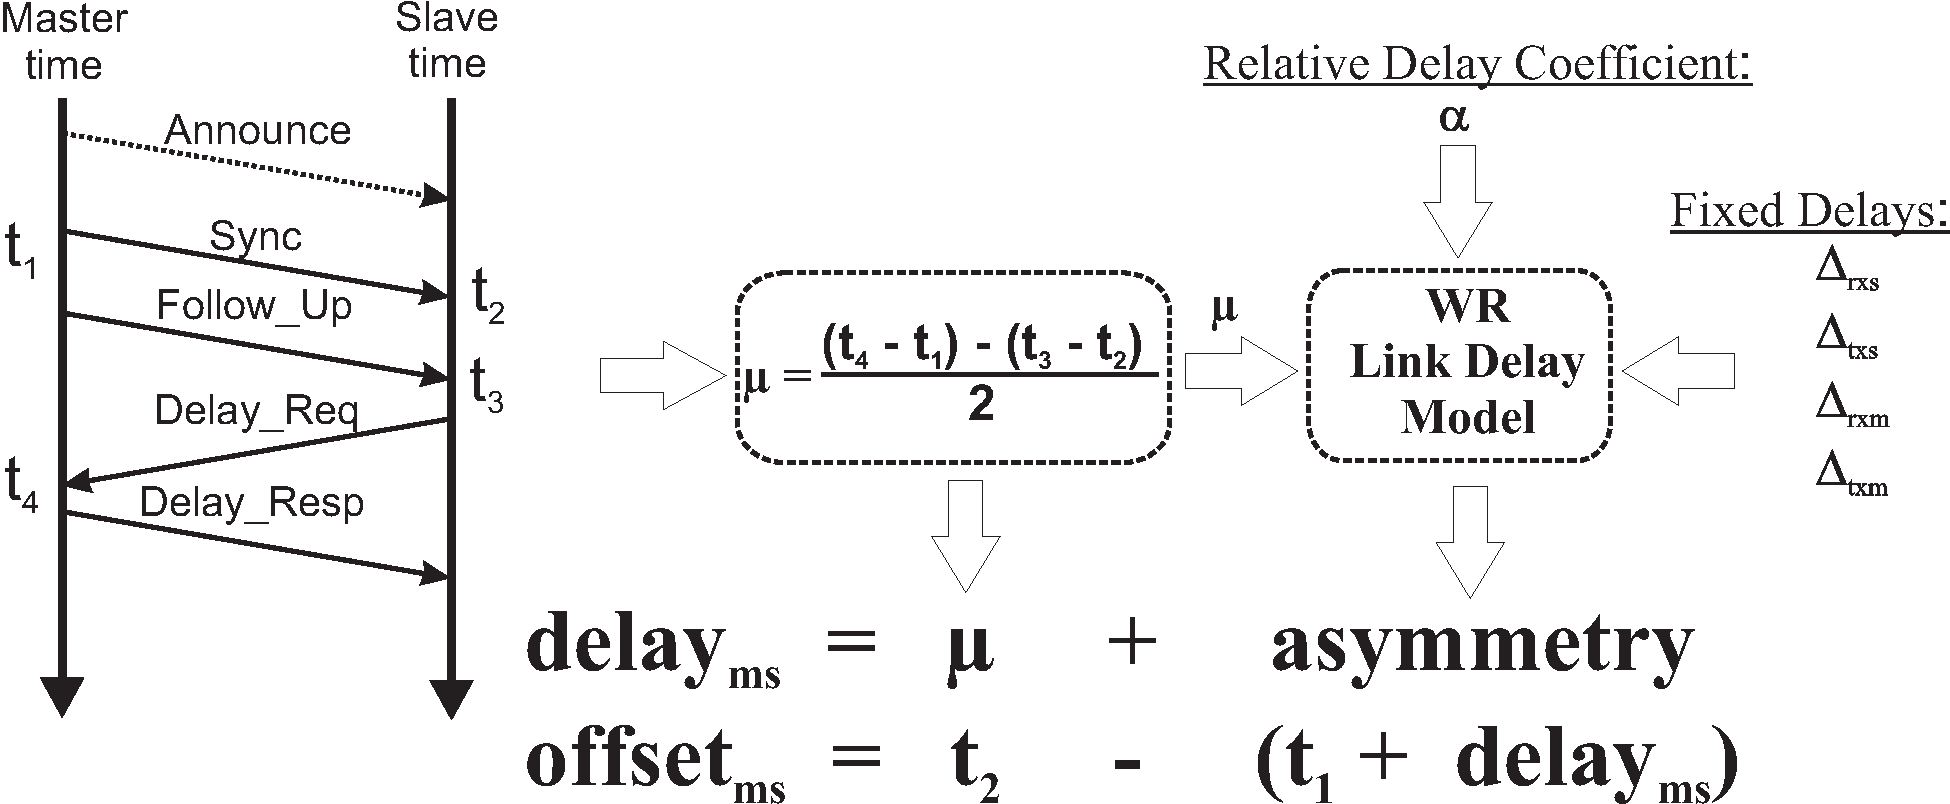
\includegraphics[height=4cm]{../../figures/protocol/wrLinkModel.eps}
  \end{center}

  \begin{columns}[c]
  \column{1.5in}

    \begin{center}
      \textbf{Solution for Ethernet over a Single-mode Optical Fiber}
    \end{center}    

  \column{2.7in}

    \begin{equation}
      \nonumber asymmetry = \Delta_{tx_m} + \Delta_{rx_s} - \frac{\Delta - \alpha \mu + \alpha \Delta}{2 + \alpha}
    \end{equation}

  \end{columns}

\end{frame}
%%%%%%%%%%%%%%%%%%%%%%%%%%%%%%%%%%%%%%%%%%%%%%%%%%%%%%%%%%%%%%%%%%%%%%%%%%%%%%%%%%%%%%%%%%%%%%%%%%%
%\section{PTP\&SyncE}
% \subsection{}
%%%%%%%%%%%%%%%%%%%%%%%%%%%%%%%%%%%%%%%%%%%%%%%%%%%%%%%%%%%%%%%%%%%%%%%%%%%%%%%%%%%%%%%%%%%%%%%%%%%%
\begin{frame}{PTP and SyncE in WR}

  \begin{itemize}
    \item Compatibility with PTP verified
    \item Compatibility with SyncE for further study
    \item Frequency distribution aligned with PTP's logic topology
%    \item Synchronous Status Message (SSM) mechanism not supported in WR
    \item PTP's Announce messages used for WR-peers recognition
  \end{itemize}

\end{frame}
%%%%%%%%%%%%%%%%%%%%%%%%%%%%%%%%%%%%%%%%%%%%%%%%%%%%%%%%%%%%%%%%%%%%%%%%%%%%%%%%%%%%%%%%%%%%%%%%%%%%
% \section{WRPTP}
% \subsection{}
%%%%%%%%%%%%%%%%%%%%%%%%%%%%%%%%%%%%%%%%%%%%%%%%%%%%%%%%%%%%%%%%%%%%%%%%%%%%%%%%%%%%%%%%%%%%%%%%%%%%
\begin{frame}{White Rabbit extension to PTP (WRPTP)}

  \begin{itemize}
    \item WR-peers recognition
    \item Calibration (fixed delays measurement)
    \item Exchange of WR-data
    \item Support of redundancy
    \item Mapping over IEEE802.3/Ethernet
  \end{itemize}

\end{frame}

%%%%%%%%%%%%%%%%%%%%%%%%%%%%%%%%%%%%%%%%%%%%%%%%%%%%%%%%%%%%%%%%%%%%%%%%%%%%%%%%%%%%%%%%%%%%%%%%%%%%
% \subsection{}
%%%%%%%%%%%%%%%%%%%%%%%%%%%%%%%%%%%%%%%%%%%%%%%%%%%%%%%%%%%%%%%%%%%%%%%%%%%%%%%%%%%%%%%%%%%%%%%%%%%%
\begin{frame}{WR-peer recognition and WR-data exchange}

  \begin{columns}[c]
  \column{.5\textwidth} 

    \begin{center}
    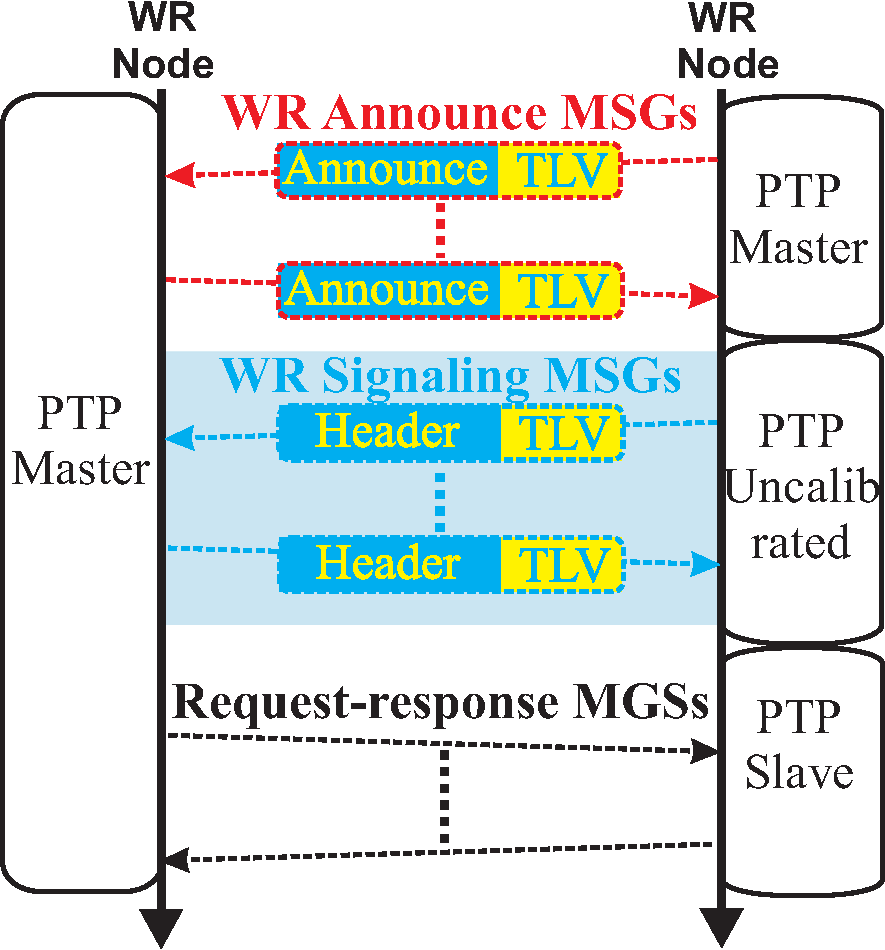
\includegraphics[width=5.0cm]{../../figures/protocol/WR-peer_recognision-1.eps}
    \newline
    Two WR devices
    \end{center}
    
  \column{.5\textwidth}

    \begin{center}
    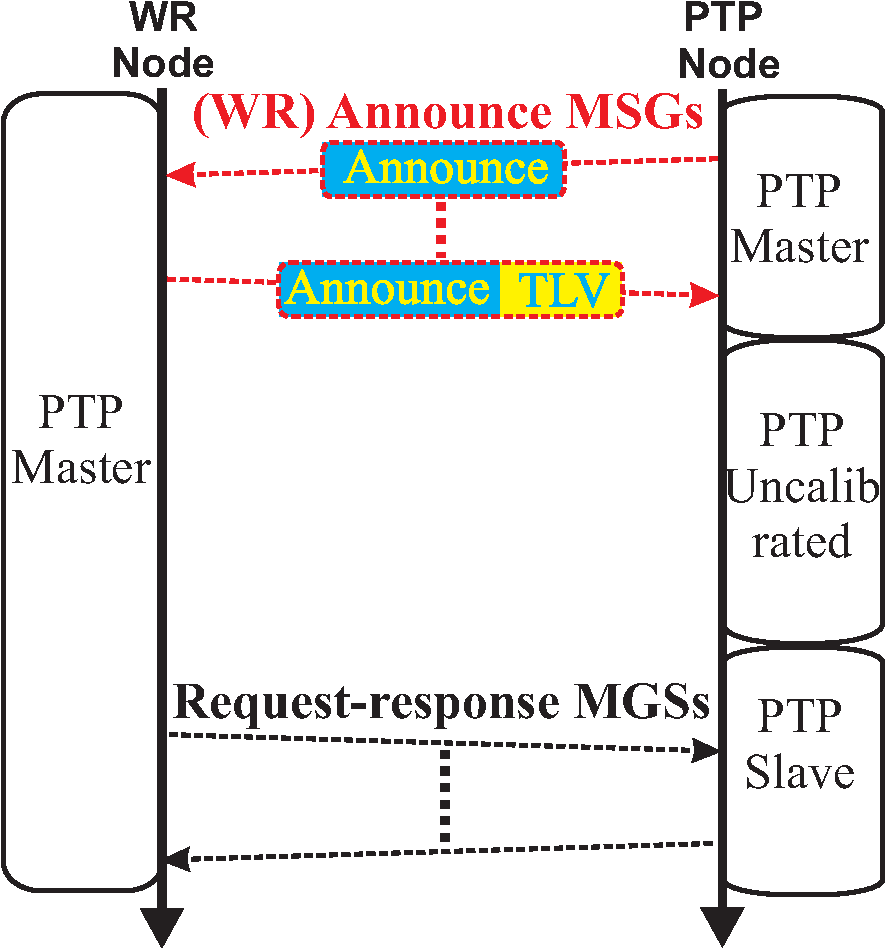
\includegraphics[width=5.0cm]{../../figures/protocol/WR-peer_recognision-2.eps}
    \newline
    WR and non-WR device
    \end{center}
     
  \end{columns}

\end{frame}
%%%%%%%%%%%%%%%%%%%%%%%%%%%%%%%%%%%%%%%%%%%%%%%%%%%%%%%%%%%%%%%%%%%%%%%%%%%%%%%%%%%%%%%%%%%%%%%%%%%%
% \subsection{}
%%%%%%%%%%%%%%%%%%%%%%%%%%%%%%%%%%%%%%%%%%%%%%%%%%%%%%%%%%%%%%%%%%%%%%%%%%%%%%%%%%%%%%%%%%%%%%%%%%%%
\begin{frame}{WR Link Setup }

  \begin{columns}[c]
  \column{.5\textwidth} 

      \begin{center}
      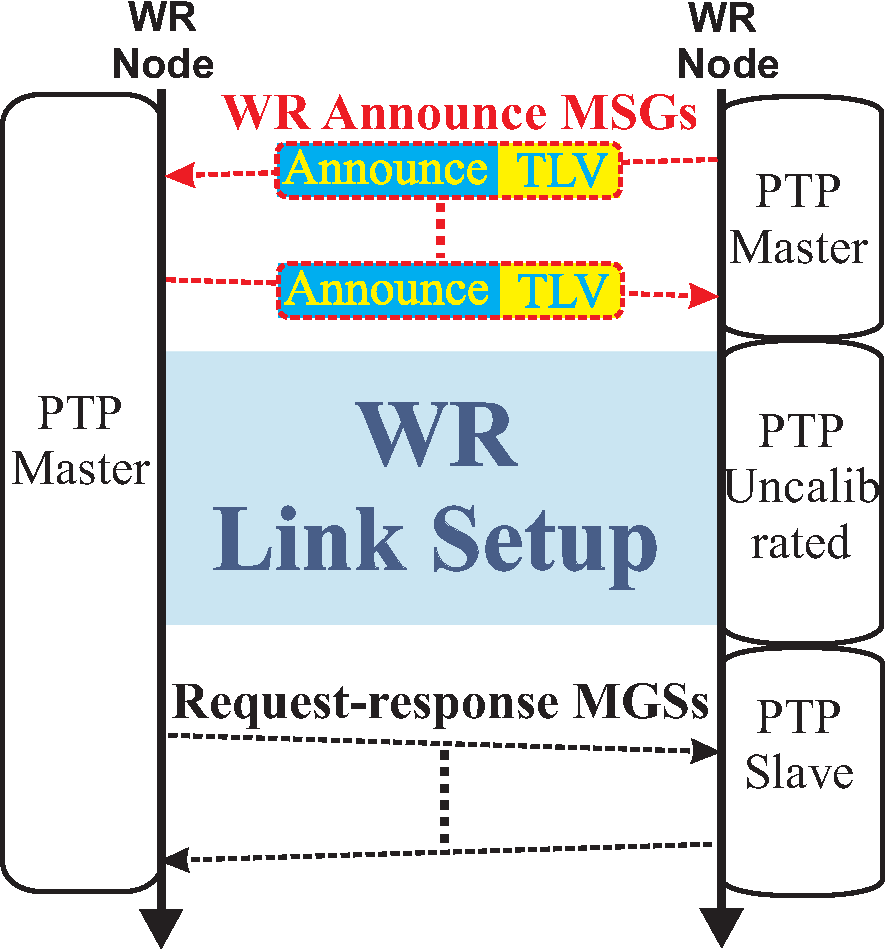
\includegraphics[width=5.5cm]{../../figures/protocol/wrLinkSetup.eps}
      \end{center}


  \column{.5\textwidth} 

      \begin{itemize}
	\item Frequency locking
	\item Calibration
	\item Exchange of WR-parameters
	\item WR Finite State Machine
	\item WR Signaling Messages
      \end{itemize}

  \end{columns}

\end{frame}

%%%%%%%%%%%%%%%%%%%%%%%%%%%%%%%%%%%%%%%%%%%%%%%%%%%%%%%%%%%%%%%%%%%%%%%%%%%%%%%%%%%%%%%%%%%%%%%%%%%%
% \subsection{}
%%%%%%%%%%%%%%%%%%%%%%%%%%%%%%%%%%%%%%%%%%%%%%%%%%%%%%%%%%%%%%%%%%%%%%%%%%%%%%%%%%%%%%%%%%%%%%%%%%%%
\begin{frame}{Modified Best Master Clock Algorithm (mBMCA)}

    \begin{center}
    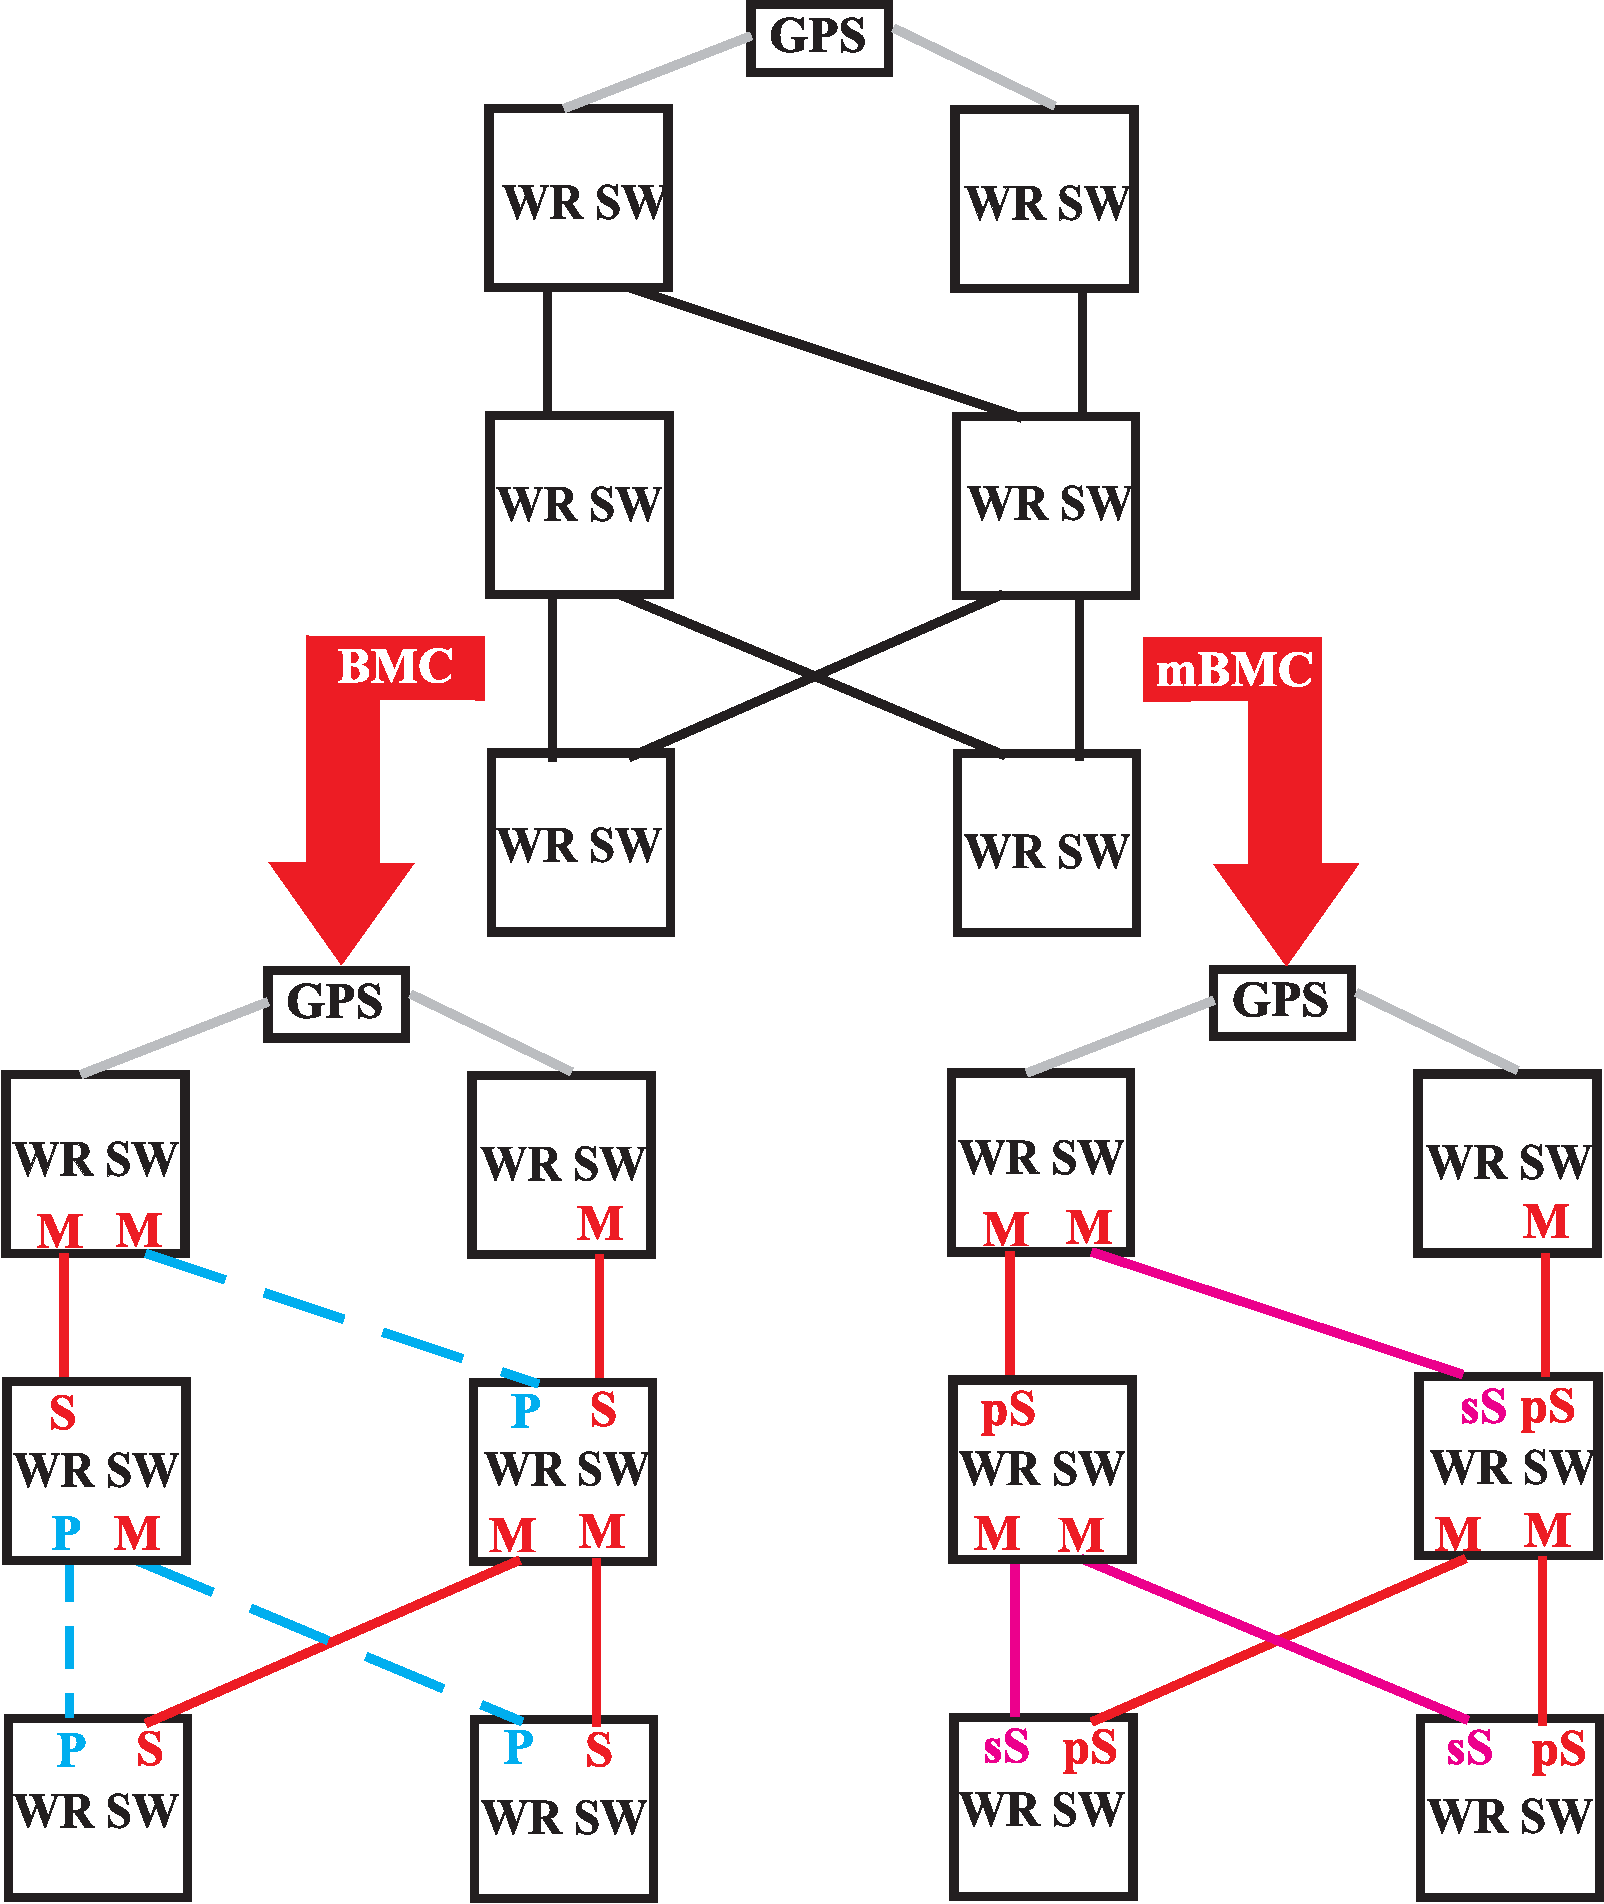
\includegraphics[height=7.0cm]{../../figures/protocol/mBMCvsBMC.eps}
    \end{center}


\end{frame}
%%%%%%%%%%%%%%%%%%%%%%%%%%%%%%%%%%%%%%%%%%%%%%%%%%%%%%%%%%%%%%%%%%%%%%%%%%%%%%%%%%%%%%%%%%%%%%%%%%%%
% \section{H/W for WR}
% \subsection{H/W for WR}
%%%%%%%%%%%%%%%%%%%%%%%%%%%%%%%%%%%%%%%%%%%%%%%%%%%%%%%%%%%%%%%%%%%%%%%%%%%%%%%%%%%%%%%%%%%%%%%%%%%%
\begin{frame}{Clock Recovery System and mBMCA}

%{\it [problem with a presentation flow]}

  \begin{center}
  \includegraphics[width=11.8cm]{../../figures/protocol/wrCRS+mBMC.eps}
  \end{center}

\end{frame}




\backupend

%%%%%%%%%%%%%%%%%%%%%%%%%%%%%%%%%%%%%%%%%%%%%%%%%%%%%%%%%%%%%%%%%%%%%%%%%%%%%%%%%%%%%%%%%%%%%%%%%%%%%%%
\end{document}
%%%%%%%%%%%%%%%%%%%%%%%%%%%%%%%%%%%%%%%%%%%%%%%%%%%%%%%%%%%%%%%%%%%%%%%%%%%%%%%%%%%%%%%%%%%%%%%%%%%%%%%